\documentclass[a4paper, 12pt, twoside]{article}
\usepackage[utf8]{inputenc}
\usepackage[T1]{fontenc}
\usepackage[french]{babel}
\usepackage{lmodern}
\usepackage{ae,aecompl}
\usepackage[top=2.5cm, bottom=2cm,
            left=3cm, right=2.5cm,
            headheight=15pt]{geometry}
\usepackage{graphicx}
\usepackage{eso-pic}
\usepackage{array}
\usepackage{booktabs}
\usepackage{longtable}
\usepackage{hyperref}
\usepackage{amsmath,amssymb}
\usepackage{microtype}
\usepackage{xcolor}
\usepackage{soul}
\usepackage{etoolbox}
\usepackage{calc}
\usepackage{xurl}
\urlstyle{same}

\input{pagedegarde}
\title{TradeDesk --- Simulateur de Place Boursière}
\entreprise{Université Paris Nanterre}
\datedebut{10 mars 2026}
\datefin{23 mai 2026}
\membrea{CHABCHOUB Younes --- N\degre{} Étudiant : 45010581}
\membreb{SAMASSEKOU Mamadou --- N\degre{} Étudiant : 45002539}
\membrec{DUFOURCQ Timothée --- N\degre{} Étudiant : 45006171}
\membred{KOSSONOU Élisée --- N\degre{} Étudiant : 45011330}
\membree{Dépôt GitHub : \url{https://github.com/TradeDesk-Mety/Projet-Informatique-L1} \\
         Application en ligne : \url{https://tradedesk-mety.streamlit.app/}}

\begin{document}
\pagedegarde

\section*{Remerciements}
Nous tenons à remercier Monsieur DELBOT pour son enseignement de l'informatique et l'opportunité de faire ce projet ainsi que Madame SAOULI qui nous a accompagné en travaux dirigés tout le long du second semestre.

\newpage
\tableofcontents
\newpage

\section{Introduction}

\subsection{Contexte et motivation}

Les marchés financiers sont souvent perçus comme inaccessibles, réservés à des professionnels maîtrisant des outils complexes et des données en temps réel. C'est précisément ce constat qui nous a poussés à développer TradeDesk : un simulateur de place boursière pédagogique permettant à n'importe quel utilisateur d'investir sur plus de 1 000 actifs réels sans risque financier.

Ce projet nous est venu par notre intérêt commun pour les marchés boursiers et par notre Double-Licence Mathématiques-Économie, qui nous a donné envie de combiner les mathématiques financières et l'informatique. L'application offre un capital virtuel choisi à l'inscription, des cours récupérés en temps quasi-réel, des indicateurs techniques (RSI, SMA et VWAP), un moteur de backtesting, un bot de trading algorithmique intégrant du Machine Learning, un pricer d'options Black-Scholes et un assistant financier conversationnel.

Les liens du projet sont les suivants :
\begin{itemize}
    \item Dépôt GitHub :
          \url{https://github.com/TradeDesk-Mety/Projet-Informatique-L1}
    \item Application en ligne :
          \url{https://tradedesk-mety.streamlit.app/}
\end{itemize}

\subsection{Objectifs généraux}

Les objectifs que nous nous sommes fixés en début de projet étaient les
suivants :

\begin{itemize}
    \item Développer une interface web professionnelle, accessible depuis
          un navigateur, sans installation côté utilisateur.
    \item Implémenter un module d'authentification sécurisé.
    \item Proposer la visualisation en temps réel des cours boursiers,
          accompagnée d'indicateurs techniques (RSI, MACD, Bollinger, VWAP).
    \item Permettre la gestion d'un portefeuille fictif multi-actifs
          (actions, ETF, options, cryptomonnaies) avec multi-portefeuilles
          par compte.
    \item Implémenter un moteur de backtesting permettant d'évaluer les
          stratégies SMA, RSI et VWAP sur données historiques.
    \item Développer un bot de trading algorithmique intégrant du Machine
          Learning (Random Forest) avec optimisation de paramètres via un
          moteur C++.
    \item Pricer des options financières européennes grâce au modèle de
          Black-Scholes.
    \item Stocker toutes les données utilisateurs dans une base de données.
\end{itemize}

\section{Environnement de travail}

\subsection{Outils de développement}

\begin{table}[h]
\begin{center}
\begin{tabular}{|p{0.4\linewidth}|p{0.5\linewidth}|}
\hline
\textbf{Outil} & \textbf{Rôle} \\
\hline
Visual Studio Code & Éditeur de code principal (extensions Python, Git, C++) \\
\hline
GitHub & Hébergement du dépôt, revue de code, gestion des branches \\
\hline
Supabase & Gestion des bases de données en ligne \\
\hline
Google Docs & Rédaction des notes de conception et du rapport \\
\hline
GitHub Codespaces & Environnement de développement cloud \\
\hline
Python & Langage de code principal du projet \\
\hline
C++ & Langage utilisé pour les calculs mathématiques \\
\hline
Streamlit & Framework Python pour applications web interactives \\
\hline
\end{tabular}
\end{center}
\caption{Outils et technologies utilisés}
\label{tab:outils}
\end{table}

\subsection{Organisation de l'équipe}

Nous nous sommes retrouvés à la bibliothèque lorsque cela était
possible, mais la majorité du projet s'est déroulée lors d'appels sur
Discord. La répartition du travail s'est déroulée de cette façon :

\begin{itemize}
    \item Appel vocal pour définir l'idée principale du projet, sa
          structure, et les langages à utiliser.
    \item Timothée et Mamadou se sont concentrés sur la logique de
          trading et d'analyse. Timothée a développé l'intégralité du
          Bot de trading, y compris le Machine Learning (Random Forest)
          et le moteur de backtesting, en implémentant l'optimisation
          des paramètres via le Grid Search en C++. Mamadou s'est chargé
          de la Page Marché (tous les graphiques Plotly, y compris les
          chandeliers et les volumes), du calcul des indicateurs
          techniques (RSI, SMA, Bollinger, VWAP) et des onglets de
          statistiques associés.
    \item Younes et Élisée se sont occupés de l'infrastructure et des
          fonctionnalités utilisateur. Younes a géré l'architecture
          globale, la base de données (Supabase), la conversion EUR/USD,
          la page Dérivés (pricing Black-Scholes), les calculs rapides
          en C++ qui y sont liés, ainsi que l'assistant financier.
          Élisée a développé la Page Portefeuille (logique d'achat/vente,
          positions, historique), le système d'authentification
          (inscription/connexion) et la gestion des portefeuilles
          utilisateurs.
    \item L'IA a été utilisée après la création des fonctions et les
          appels associés.
    \item Puis nous avons fait un appel vocal général où nous avons
          corrigé les bugs du site et fait les ajouts de dernière minute
          pour rendre l'utilisation du site la plus fluide possible.
\end{itemize}

\section{Description du projet et objectifs}

\subsection{Qu'est-ce que le paper trading ?}

Le paper trading (ou trading fictif) consiste à simuler des opérations
boursières --- achats et ventes d'actifs financiers --- sans engager de
capitaux réels. C'est un outil pédagogique largement utilisé par les
professionnels pour tester des stratégies avant de les appliquer en
conditions réelles, et par les débutants pour apprendre les mécanismes
des marchés sans risque financier.

TradeDesk suit cette logique : chaque utilisateur dispose d'un capital
virtuel qu'il choisit lui-même à l'inscription (de 1~000 à 1~000~000
euros fictifs), et peut l'investir sur plus de 1~000 actifs réels dont
les cours sont récupérés en temps quasi-réel.

\subsection{Architecture générale}

Le projet suit une architecture en couches bien séparées, conçue pour
être maintenable et extensible :

\begin{verbatim}
Projet-Informatique-L1/
├── .devcontainer/    -> Configuration GitHub Codespaces
├── .streamlit/       -> Configuration Streamlit (thème + secrets)
├── bot/              -> Bot de trading algorithmique
├── data/             -> Pipeline Medallion + sécurité
├── equities/         -> Gestion du portefeuille utilisateur
├── finance/          -> Moteur de calcul C++ + wrapper Python
├── greeks/           -> Formules Black-Scholes et Greeks
├── simulation/       -> Backtesting et Monte-Carlo
├── tests/            -> Suite de tests unitaires
├── visualisation/    -> Graphiques interactifs Plotly
├── website/          -> Application web Streamlit
├── launch.sh         -> Script de lancement Linux/macOS
├── Lancer_TradeDesk.bat -> Script de lancement Windows
└── requirements.txt  -> Dépendances Python
\end{verbatim}

\subsection{Les pages du site web}

\begin{table}[h]
\begin{center}
\begin{tabular}{|p{0.3\linewidth}|p{0.6\linewidth}|}
\hline
\textbf{Page} & \textbf{Fonctionnalité principale} \\
\hline
TradeDesk (accueil) & Authentification, inscription \\
\hline
Marché & Analyse en temps réel, indicateurs techniques, corrélations \\
\hline
Portefeuille & Gestion des ordres, positions, historique, multi-portefeuilles \\
\hline
Backtesting & Test des stratégies SMA, RSI, VWAP sur données historiques \\
\hline
Bot & Trading algorithmique automatisé (ML inclus) \\
\hline
Dérivés & Pricing d'options Black-Scholes, surface 3D, Greeks \\
\hline
Assistant & Conseiller financier conversationnel \\
\hline
Documentation & Mode d'emploi complet, cours de finance \\
\hline
Paramètres & Profil, sécurité, gestion des portefeuilles \\
\hline
\end{tabular}
\end{center}
\caption{Pages de l'application TradeDesk}
\label{tab:pages}
\end{table}

\section{Bibliothèques, Outils et Technologies}

\subsection{Langage principal : Python}

L'intégralité du code applicatif est écrite en Python. Ce choix s'est
fait naturellement : Python est le langage de référence pour le
traitement de données financières, et dispose d'un écosystème de
bibliothèques exceptionnel. De plus, il nous a été enseigné dans notre
formation dans le cadre du cours Algorithme et Mise en Œuvre
Informatique.

\subsection{Framework web : Streamlit}

Streamlit est un framework Python open-source permettant de créer des
applications web interactives sans écrire une seule ligne de HTML ou
JavaScript. Il transforme des scripts Python en applications web
réactives grâce à un modèle déclaratif.

Nous avons exploité les fonctionnalités avancées de Streamlit : gestion
de l'état de session (\texttt{st.session\_state}), cache de données avec
TTL (\texttt{@st.cache\_data}), colonnes responsives, onglets, métriques,
formulaires, et injection de CSS personnalisé via
\texttt{st.markdown(unsafe\_allow\_html=True)}.

\subsection{Données de marché : yfinance}

yfinance est une bibliothèque Python permettant d'accéder gratuitement
aux données de Yahoo Finance. Elle fournit les historiques OHLCV\footnote{Open, High, Low, Close, Volume --- Prix d'Ouverture, Plus Haut Prix, Plus Bas Prix, Prix de Fermeture et Volume des transactions.},
les cours en temps quasi-réel et les métadonnées des actifs. Nous avons
intégré plus de 1~000 actifs dans notre dictionnaire \texttt{MARKET} :
500 actions américaines, 500 actions européennes (suffixes
\texttt{.PA}, \texttt{.BR}, \texttt{.MI}\ldots), des ETF, indices et
cryptomonnaies.

\subsection{Visualisation : Plotly}

Plotly est une bibliothèque de visualisation interactive. Nous avons
développé 10 types de graphiques personnalisés : chandeliers japonais
(OHLCV) avec indicateurs superposés, surfaces 3D Black-Scholes, heatmap
de corrélation, jauge RSI animée, distribution des rendements vs loi
normale, etc. Tous les graphiques utilisent un thème sombre unifié
cohérent avec l'interface de l'application.

\subsection{Base de données : PostgreSQL et Supabase}

Les données utilisateurs (comptes, portefeuilles, positions,
transactions) sont stockées dans une base PostgreSQL hébergée sur
Supabase (infrastructure cloud), accessible via la bibliothèque
\texttt{psycopg2}. Le schéma comprend 8 tables relationnelles avec
contraintes de clé étrangère et cascade de suppression.

\subsection{Moteur de calcul : C++ via ctypes}

Pour les calculs intensifs (Grid Search des paramètres de trading,
pricing Black-Scholes), nous avons développé un moteur C++ compilé en
bibliothèque partagée (\texttt{.so} / \texttt{.dylib} / \texttt{.dll})
et appelé depuis Python via \texttt{ctypes}. La compilation est
automatique au premier lancement (\texttt{g++} ou \texttt{clang++}).
Un fallback Python pur est disponible si aucun compilateur n'est détecté.

\subsection{Machine Learning : scikit-learn}

Le bot de trading en mode ML utilise un Random Forest de scikit-learn,
entraîné sur des features techniques (SMA, RSI, VWAP, rendements). La
qualité du modèle est évaluée par validation croisée 5-Folds. Les
probabilités brutes sont recalibrées par Platt Scaling (régression
logistique) pour corriger le biais des forêts aléatoires sur la sortie
probabiliste.

\subsection{Sécurité : PBKDF2-HMAC-SHA256}

L'authentification repose sur le hachage des mots de passe avec
l'algorithme PBKDF2-HMAC-SHA256 de la bibliothèque standard Python
(\texttt{hashlib}) :

\begin{itemize}
    \item Sel aléatoire de 16 octets (\texttt{os.urandom(16)}) généré à
          chaque inscription.
    \item 100~000 itérations (recommandation NIST 2023).
    \item Comparaison en temps constant via \texttt{hmac.compare\_digest()}
          (protection contre les timing attacks).
\end{itemize}

\begin{table}[h]
\begin{center}
\begin{tabular}{|p{0.35\linewidth}|p{0.55\linewidth}|}
\hline
\textbf{Bibliothèque} & \textbf{Usage} \\
\hline
streamlit & Interface web \\
\hline
yfinance & Données de marché Yahoo Finance \\
\hline
pandas & Manipulation de données tabulaires \\
\hline
numpy & Calculs numériques vectorisés \\
\hline
plotly & Graphiques interactifs \\
\hline
scipy & Loi normale (Black-Scholes) \\
\hline
scikit-learn & Machine Learning (Random Forest) \\
\hline
psycopg2-binary & Connexion PostgreSQL \\
\hline
difflib & Recherche floue dans l'assistant \\
\hline
hashlib & Hachage PBKDF2-SHA256 des mots de passe \\
\hline
ctypes & Interface C++ $\leftrightarrow$ Python \\
\hline
\end{tabular}
\end{center}
\caption{Récapitulatif des bibliothèques Python utilisées}
\label{tab:libs}
\end{table}

\section{Travail réalisé}

\subsection{Fonctionnalités réalisées}

L'ensemble des fonctionnalités initialement prévues a été implémenté.
Nous les détaillons ci-dessous par module.

\textbf{Authentification :}

Le système d'authentification permet à un utilisateur de créer un compte
avec un nom d'utilisateur unique et un mot de passe (vérification de la
disponibilité du pseudo, confirmation du mot de passe), puis de se
connecter. Le capital initial fictif est choisi librement à l'inscription
via un slider (de 1~000 à 1~000~000 euros). Les mots de passe sont
hachés avec PBKDF2-HMAC-SHA256 avant stockage --- aucun mot de passe en
clair ne transite dans le système. La session utilisateur est maintenue
via \texttt{st.session\_state}, avec déconnexion sécurisée.

\textbf{Analyse de marché (page Marché) :}

La page Marché est la plus riche de l'application. Elle propose six
sous-onglets :

\begin{itemize}
    \item \textbf{Temps Réel :} Affichage des prix des actifs mis à jour
          en continu avec sélection de l'intervalle (de la minute à la
          semaine), indicateur VWAP et jauge RSI animée.
    \item \textbf{Historique :} Chandeliers japonais avec Bandes de
          Bollinger et volume coloré selon la direction du marché.
    \item \textbf{Volatilité \& Volume :} Mesure de la volatilité
          annualisée en continu, avec alertes en cas de volume
          exceptionnellement élevé.
    \item \textbf{Statistiques :} Ratio de Sharpe, volatilité, Bêta
          (référence S\&P~500), Skewness et Kurtosis, mis à jour
          instantanément au changement de période.
    \item \textbf{Rendements :} Distribution réelle des rendements
          comparée à la loi normale théorique.
    \item \textbf{Corrélation :} Heatmap Pearson permettant de comparer
          la co-évolution de plusieurs actifs sélectionnés librement.
\end{itemize}

Les cours des actifs cotés en USD sont automatiquement convertis en
euros au taux EUR/USD en temps réel.

\textbf{Gestion du portefeuille (page Portefeuille) :}

\begin{itemize}
    \item \textbf{Actions / ETF :} Achat ou vente de parts entières
          d'entreprises ou de paniers d'actifs.
    \item \textbf{Cryptomonnaies :} Achat de montants très précis,
          y compris de très petites fractions (par exemple, 0,001 BTC).
    \item \textbf{Options (Call / Put) :} Contrats donnant le droit
          d'acheter (Call) ou de vendre (Put) un actif à un prix fixé
          d'avance (Strike) et à une date future (1, 3, 6 ou 12~mois).
          Le prix est calculé automatiquement via Black-Scholes.
\end{itemize}

Une commission fixe de 1~\% est retenue sur chaque transaction. Les
calculs sont effectués via le moteur C++. Le tableau récapitulatif
affiche le PAMP, le prix actuel, et les gains/pertes latents avec
coloration dynamique. L'historique complet est exportable en CSV.
La fonctionnalité multi-portefeuilles permet de gérer plusieurs comptes
indépendants, nommables et supprimables.

\textbf{Backtesting (page Backtesting) :}

Le moteur de backtesting simule trois stratégies algorithmiques sur des
données historiques réelles :

\begin{itemize}
    \item \textbf{SMA :} Achat/vente sur croisement de moyennes mobiles
          (Golden Cross).
    \item \textbf{RSI :} Achat quand l'actif est survendu, vente quand
          il est suracheté (seuils configurables).
    \item \textbf{VWAP :} Achat si le prix est inférieur au VWAP, vente
          s'il le dépasse.
\end{itemize}

Le système fournit des métriques de performance (gain total, perte
maximale, etc.) et peut optimiser automatiquement les paramètres via le
Grid Search en C++.

\textbf{Bot de trading (page Bot) :}

Le bot propose quatre modes de fonctionnement :

\begin{enumerate}
    \item \textbf{SMA :} Décision basée sur le croisement de moyennes
          mobiles avec paramètres optimisés automatiquement.
    \item \textbf{RSI :} Décision basée sur l'indicateur de
          survente/surachat, paramètres optimisés automatiquement.
    \item \textbf{VWAP :} Décision par rapport au prix moyen pondéré
          par les volumes, paramètres optimisés automatiquement.
    \item \textbf{Machine Learning :} Modèle Random Forest entraîné
          sur des features techniques, validé par validation croisée
          5-Folds et calibré par Platt Scaling.
\end{enumerate}

Avant tout ordre, le bot génère un rapport complet (analyse technique,
signal détecté, niveau de confiance, risque estimé). Aucun ordre ne peut
être exécuté sans validation explicite de l'utilisateur.

\textbf{Pricing d'options et Greeks (page Dérivés) :}

La page Dérivés implémente le modèle de Black-Scholes (1973) pour le
pricing d'options européennes Call et Put. Elle calcule et affiche les
cinq Greeks :

\begin{table}[h]
\begin{center}
\begin{tabular}{|c|c|p{0.5\linewidth}|}
\hline
\textbf{Greek} & \textbf{Symbole} & \textbf{Interprétation} \\
\hline
Delta & $\Delta$ & Sensibilité au prix du sous-jacent \\
\hline
Gamma & $\Gamma$ & Variation du Delta \\
\hline
Vega  & $\nu$    & Sensibilité à la volatilité \\
\hline
Theta & $\Theta$ & Décroissance temporelle \\
\hline
Rho   & $\rho$   & Sensibilité aux taux d'intérêt \\
\hline
\end{tabular}
\end{center}
\caption{Les cinq Greeks calculés dans TradeDesk}
\label{tab:greeks}
\end{table}

La page comprend également une surface 3D interactive du prix de
l'option en fonction du Strike et de la Maturité, un Volatility Smile,
et les courbes de sensibilité des Greeks.

\textbf{Assistant financier (page Assistant) :}

L'assistant conversationnel est un chatbot à base de règles enrichi. Il
peut :

\begin{itemize}
    \item Expliquer plus de 40 concepts financiers (RSI, VWAP, Sharpe,
          Black-Scholes, options, PEA, etc.) avec recherche floue
          (\texttt{difflib}) pour tolérer les fautes de frappe.
    \item Recommander des actifs basé sur le Ratio de Sharpe calculé
          en temps réel sur un an de données.
    \item Consulter le portefeuille actif et lister tous les
          portefeuilles de l'utilisateur.
    \item Effectuer des calculs mathématiques en langage naturel
          (ex.~«~5~\% de 2~000~»).
    \item Afficher le taux EUR/USD en temps réel.
\end{itemize}

\textbf{Documentation et Paramètres :}

La page Documentation comprend cinq sous-onglets : Mode d'Emploi,
Comprendre les Graphiques, Stratégies \& Indicateurs (avec formules
mathématiques), Cours de Finance accéléré (6 chapitres), et Glossaire
(60+ termes avec recherche). La page Paramètres permet la modification
du mot de passe, la gestion des portefeuilles et la suppression du
compte avec double confirmation.

\subsection{Fonctionnalités non réalisées}

\begin{table}[h]
\begin{center}
\begin{tabular}{|p{0.45\linewidth}|p{0.45\linewidth}|}
\hline
\textbf{Fonctionnalité prévue} & \textbf{Raison de la non-réalisation} \\
\hline
Authentification par e-mail avec A2F &
    Complexité d'intégration d'un serveur SMTP en environnement
    Streamlit Cloud gratuit \\
\hline
Intégration d'actualités géopolitiques pour enrichir l'assistant &
    Absence d'API gratuite fiable et structurée pour l'analyse de
    sentiment en temps réel \\
\hline
Récupération de mot de passe &
    Nécessite un système d'e-mail, reporté à une version future \\
\hline
Affichage des données en direct &
    Impossible avec yfinance (données quasi-temps réel uniquement) \\
\hline
\end{tabular}
\end{center}
\caption{Fonctionnalités prévues non réalisées}
\label{tab:nonrealise}
\end{table}

\subsection{Répartition du travail}

La répartition suivante reflète la contribution réelle de chaque membre
du groupe :

\begin{itemize}
    \item \textbf{CHABCHOUB Younes :} Architecture globale du projet,
          migration de la base de données vers Supabase (PostgreSQL
          cloud), système multi-portefeuilles, conversion EUR/USD, page
          Dérivés et pricing Black-Scholes, assistant financier, pages
          légales, corrections de bugs transverses.
    \item \textbf{SAMASSEKOU Mamadou :} Page Marché (tous les graphiques
          Plotly), calcul des indicateurs techniques (RSI, SMA, Bollinger,
          VWAP), onglets Volatilité \& Volume, Statistiques et
          Corrélation, script \texttt{visualisation.py}.
    \item \textbf{KOSSONOU Élisée :} Page Portefeuille (ordres,
          positions, historique), intégration des cryptomonnaies comme
          catégorie d'instrument, système d'authentification, page
          Paramètres, pipeline Medallion Bronze $\to$ Silver $\to$ Gold.
    \item \textbf{DUFOURCQ Timothée :} Bot de trading (stratégies SMA,
          RSI, VWAP, ML), moteur de backtesting, Grid Search C++
          (implémentation ctypes), Random Forest avec calibration, page
          Documentation, suite de tests unitaires et déploiement
          Streamlit Cloud.
    \item \textbf{Rôle de l'IA :} Nous avons dans un premier temps créé
          le site sans utilisation de l'IA, en nous appuyant sur la
          documentation Streamlit et nos connaissances en C++ et en
          Python. L'IA est ensuite intervenue en tant qu'assistant de
          programmation : après avoir pris connaissance de notre travail
          existant et du cahier des charges, elle a proposé des
          améliorations ciblées sur des points clés (intégration de
          \texttt{ctypes}, gestion de l'état Streamlit, calculs
          financiers). Son utilisation s'est toujours faite sous notre
          supervision et a nécessité un sens critique constant pour
          valider ses suggestions.
\end{itemize}

\section{Difficultés rencontrées}

\subsection{Compatibilité période / intervalle dans yfinance}

L'API yfinance impose des contraintes strictes sur les combinaisons
période / intervalle : les données à la minute ne sont disponibles que
sur 7 jours maximum, et les données horaires sur 60 jours au plus. Gérer
ces contraintes sans planter l'application a nécessité l'implémentation
d'un système d'avertissements et de messages d'erreur clairs pour
l'utilisateur. De plus, certains actifs européens ne disposent pas de
données de volume via yfinance, ce qui a nécessité des vérifications
supplémentaires avant tout rendu graphique.

\subsection{Migration de la base de données en production}

La base de données était initialement conçue avec un schéma simple (un
seul portefeuille par utilisateur, clé primaire \texttt{user\_id} sur la
table \texttt{portfolio\_state}). L'ajout de la fonctionnalité
multi-portefeuilles en cours de développement a nécessité une migration
du schéma en base déjà en production sur Supabase, sans pouvoir effacer
les données existantes. Nous avons dû écrire des scripts de migration
rétrocompatibles utilisant \texttt{ALTER TABLE ... ADD COLUMN IF NOT
EXISTS} et des blocs \texttt{DO \$\$} PostgreSQL pour modifier les
contraintes de clé primaire à chaud.

\subsection{Gestion de l'état Streamlit entre les pages}

Streamlit réexécute l'intégralité du script Python à chaque interaction
de l'utilisateur. La gestion de l'état entre les pages --- notamment le
portefeuille actif, l'utilisateur connecté et le portefeuille sélectionné
--- a nécessité une utilisation avancée de \texttt{st.session\_state} et
une attention particulière à l'ordre d'initialisation des variables pour
éviter les \texttt{KeyError} ou les rechargements intempestifs.

\subsection{Compilation C++ multi-plateforme}

Le moteur de calcul C++ devait fonctionner sur macOS (M1/M2), Linux
(Streamlit Cloud) et Windows. Les trois systèmes utilisent des
compilateurs, des conventions d'appel et des extensions de fichier
différents (\texttt{.dylib}, \texttt{.so}, \texttt{.dll}). Nous avons
implémenté une logique de détection automatique du compilateur disponible
(\texttt{g++}, \texttt{clang++}) et du système d'exploitation, avec
fallback Python pur si nécessaire. La compilation automatique à la volée
a posé des problèmes de droits sur Streamlit Cloud, résolus en
distribuant le binaire pré-compilé Linux dans le dépôt.

\section{Bilan}

\subsection{Conclusion}

D'un point de vue technique, nous avons acquis des compétences concrètes
en développement web Python (Streamlit), en gestion de bases de données
relationnelles (PostgreSQL, psycopg2), en cryptographie appliquée
(PBKDF2), en visualisation de données (Plotly), en mathématiques
financières (Black-Scholes, Greeks, backtesting) et en Machine Learning
(Random Forest, calibration). L'intégration d'un moteur C++ via
\texttt{ctypes} pour les calculs intensifs a également été une étape
importante pour comprendre les relations entre les différents langages.

D'un point de vue méthodologique, ce projet nous a confrontés aux
réalités du développement en équipe : gestion de conflits Git,
coordination des tâches, revue de code, et surtout la nécessité de
documenter et de tester son code. La programmation assistée par IA a
constitué un levier d'accélération important, mais nous a aussi appris à
exercer notre sens critique face aux suggestions automatisées.

Le déploiement en production avec de vrais utilisateurs, une base de
données cloud et des contraintes de disponibilité a ajouté une dimension
opérationnelle absente des travaux pratiques habituels.

\subsection{Perspectives}

Plusieurs axes d'amélioration ont été identifiés en cours de
développement et pourraient faire l'objet de versions futures :

\begin{itemize}
    \item \textbf{Authentification par e-mail avec A2F :} ajout d'une
          vérification d'adresse e-mail et d'une authentification à deux
          facteurs (TOTP) pour renforcer la sécurité des comptes.
    \item \textbf{Intégration d'actualités financières :} connexion à une
          API de news (NewsAPI, Reuters) avec analyse de sentiment (NLP)
          pour enrichir les recommandations du bot.
    \item \textbf{Notifications en temps réel :} alertes push lorsqu'un
          seuil de cours ou un signal de trading est franchi.
    \item \textbf{Comparaison multi-stratégies :} visualisation
          simultanée de plusieurs stratégies de backtesting sur la même
          période.
    \item \textbf{Application mobile :} adaptation de l'interface pour
          une meilleure expérience sur smartphone.
\end{itemize}

\newpage

\section{Webographie}
\renewcommand{\refname}{}
\begin{thebibliography}{10}
    \bibitem[STR]{str} Documentation officielle Streamlit.
        \url{https://docs.streamlit.io}
    \bibitem[YFI]{yfi} Documentation yfinance (Ran Aroussi).
        \url{https://github.com/ranaroussi/yfinance}
    \bibitem[PLT]{plt} Documentation Plotly Python.
        \url{https://plotly.com/python/}
    \bibitem[SKL]{skl} Documentation scikit-learn --- RandomForestClassifier.
        \url{https://scikit-learn.org/stable/modules/generated/sklearn.ensemble.RandomForestClassifier.html}
    \bibitem[SUP]{sup} Documentation Supabase PostgreSQL Cloud.
        \url{https://supabase.com/docs}
    \bibitem[PSY]{psy} Documentation psycopg2 --- PostgreSQL adapter for Python.
        \url{https://www.psycopg.org/docs/}
    \bibitem[NIST]{nist} NIST Special Publication 800-132 --- Recommendation
        for Password-Based Key Derivation.
        \url{https://csrc.nist.gov/publications/detail/sp/800-132/final}
    \bibitem[REPO]{repo} Dépôt GitHub du projet TradeDesk.
        \url{https://github.com/TradeDesk-Mety/Projet-Informatique-L1}
    \bibitem[SCR]{scr} Documentation SciPy --- scipy.stats.norm.
        \url{https://docs.scipy.org/doc/scipy/reference/generated/scipy.stats.norm.html}
    \bibitem[INVE]{inve} Investopedia --- Référence des concepts financiers.
        \url{https://www.investopedia.com}
\end{thebibliography}

\newpage

\section{Annexes}
\appendix
\makeatletter
\def\@seccntformat#1{Annexe~\csname the#1\endcsname~:\quad}
\makeatother

    \section{Cahier des charges}

    % ── A.1 Contexte ──────────────────────────────────────────────────────────
    \subsection*{A.1 Contexte et périmètre du projet}

    Lorsque nous avons débuté ce projet en mars 2026, nous partions d'une
    question simple : comment apprendre concrètement à investir en bourse
    sans prendre de risques financiers réels~? La réponse évidente était le
    \textbf{paper trading} --- simuler des opérations boursières avec un
    capital fictif, dans les mêmes conditions que les marchés réels.

    C'est de cette idée qu'est né \textbf{TradeDesk}. Plutôt que de
    développer une application générique, nous avons voulu construire quelque
    chose qui nous ressemble : une plateforme mêlant la rigueur de la finance
    quantitative, la puissance du Machine Learning et l'accessibilité d'une
    interface web moderne.

    L'application couvre l'intégralité du cycle d'un investisseur : se
    connecter, analyser les marchés, passer des ordres, tester ses
    stratégies sur l'historique, automatiser ses décisions avec un bot,
    pricer des produits dérivés et consulter un assistant financier --- le
    tout sans quitter le navigateur, sans installation, et sans risquer le
    moindre euro réel.

    % ── A.2 Acteurs ───────────────────────────────────────────────────────────
    \subsection*{A.2 Acteurs du système}

    TradeDesk a été conçu autour d'un seul type d'utilisateur humain :
    l'apprenant. Un point important : le système ne prend \textbf{jamais de
    décisions financières de façon autonome}. Le bot analyse et propose, mais
    c'est toujours l'utilisateur qui autorise ou refuse l'ordre.

    \begin{table}[h]
    \centering
    \begin{tabular}{|>{\bfseries}l|l|p{5.5cm}|}
    \hline
    Acteur & Rôle & Droits \\
    \hline
    Visiteur & Accède à la page d'accueil sans compte
             & Création de compte et connexion uniquement \\
    \hline
    Utilisateur connecté & Titulaire d'un compte avec capital virtuel
             & Toutes les fonctionnalités (marché, portefeuille, bot,
               backtesting, dérivés, assistant, paramètres) \\
    \hline
    Système (automatique) & Pipeline Medallion, bot de trading
             & Lecture/écriture en base de données, exécution des calculs \\
    \hline
    \end{tabular}
    \caption{Acteurs du système TradeDesk}
    \end{table}

    % ── A.3 Besoins fonctionnels ──────────────────────────────────────────────
    \subsection*{A.3 Besoins fonctionnels détaillés}

    \subsubsection*{BF1 --- Authentification et gestion de compte}

    L'inscription exige un pseudo unique (minimum 3~caractères), un mot de
    passe (minimum 4~caractères) saisi deux fois pour éviter les erreurs, et
    le choix d'un capital de départ fictif compris entre 1~000 et
    1~000~000~euros. Le mot de passe est haché avec
    \textbf{PBKDF2-HMAC-SHA256} (100~000~itérations, sel aléatoire de
    16~octets) avant toute persistance --- aucun mot de passe en clair ne
    transite dans le système. La comparaison lors de la connexion s'effectue
    en \textbf{temps constant} (\texttt{hmac.compare\_digest}) pour se
    protéger contre les attaques par mesure de temps.

    Une fois connecté, l'utilisateur peut modifier son mot de passe,
    supprimer son compte avec double confirmation, et gérer plusieurs
    portefeuilles indépendants depuis la page Paramètres.

    \subsubsection*{BF2 --- Analyse de marché en temps réel}

    L'utilisateur peut sélectionner n'importe quel actif parmi plus de
    \textbf{1~000~disponibles} (actions américaines et européennes, ETF,
    indices, cryptomonnaies) et l'analyser via six onglets distincts :

    \begin{itemize}
        \item \textbf{Temps Réel :} graphique du cours sur une période et un
              intervalle configurables (de~1~minute à~1~semaine), ligne VWAP
              superposée, jauge RSI animée et sélecteur de date pour
              revivre n'importe quelle séance passée.
        \item \textbf{Historique :} chandeliers japonais OHLC avec SMA20,
              SMA50, Bandes de Bollinger ($\pm 2\sigma$) et volumes colorés
              (vert/rouge selon la variation).
        \item \textbf{Volatilité \& Volume :} volatilité annualisée glissante
              et détection automatique des anomalies de volume
              (signal quand le volume dépasse $2\times$ sa moyenne sur
              20~séances).
        \item \textbf{Statistiques :} Ratio de Sharpe, volatilité annualisée,
              Bêta vs S\&P~500, Skewness et Kurtosis, recalculés
              dynamiquement selon la période choisie.
        \item \textbf{Rendements :} distribution empirique des rendements
              journaliers comparée à la loi normale ajustée.
        \item \textbf{Corrélation :} heatmap de Pearson entre actifs
              sélectionnés librement par l'utilisateur.
    \end{itemize}

    Les actifs cotés en USD sont automatiquement convertis en euros au taux
    EUR/USD récupéré en temps réel via yfinance.

    \subsubsection*{BF3 --- Gestion du portefeuille (Paper Trading)}

    L'utilisateur peut passer des ordres sur trois catégories d'instruments :
    \begin{itemize}
        \item \textbf{Actions et ETF :} quantités entières, cours en temps
              réel.
        \item \textbf{Cryptomonnaies :} quantités fractionnaires (ex.
              0,001~BTC).
        \item \textbf{Options Call/Put européennes :} pricées selon le modèle
              Black-Scholes à partir du cours du sous-jacent, du strike,
              de la maturité (1, 3, 6 ou 12~mois) et de la volatilité
              historique calculée automatiquement.
    \end{itemize}

    Une commission de \textbf{1~\%} est appliquée à chaque transaction via le
    moteur C++. Un récapitulatif (montant brut, commission, montant net) est
    affiché avant confirmation. Le tableau des positions affiche le Prix
    d'Achat Moyen Pondéré (PAMP), le cours actuel, la plus ou moins-value
    latente et le ROI avec coloration dynamique. L'historique est exportable
    au format CSV. Chaque utilisateur dispose de \textbf{plusieurs
    portefeuilles indépendants}.

    \subsubsection*{BF4 --- Backtesting de stratégies algorithmiques}

    \begin{table}[h]
    \centering
    \begin{tabular}{|>{\bfseries}l|l|l|p{3.5cm}|}
    \hline
    Stratégie & Signal d'achat & Signal de vente & Paramètres \\
    \hline
    SMA & SMA courte $>$ SMA longue & SMA courte $<$ SMA longue
        & Fenêtres courte et longue \\
    \hline
    RSI & RSI $<$ seuil de survente & RSI $>$ seuil de surachat
        & Période RSI, seuils \\
    \hline
    VWAP & Cours $<$ VWAP & Cours $>$ VWAP
         & Période de calcul \\
    \hline
    \end{tabular}
    \caption{Stratégies de backtesting disponibles}
    \end{table}

    Les métriques calculées sont : rendement total, Alpha vs Buy \& Hold,
    Max Drawdown, nombre d'ordres et commissions cumulées. Un mode comparatif
    affiche les trois stratégies simultanément. Le \textbf{Grid Search C++}
    optimise automatiquement les paramètres pour maximiser le rendement
    historique.

    \subsubsection*{BF5 --- Bot de trading algorithmique}

    Le bot analyse un actif et génère un signal (Achat / Vente / Neutre)
    selon quatre modes :
    \begin{enumerate}
        \item \textbf{Mode SMA :} croisement de moyennes mobiles, paramètres
              optimisés par Grid Search C++.
        \item \textbf{Mode RSI :} zones de surachat/survente, paramètres
              optimisés par Grid Search C++.
        \item \textbf{Mode VWAP :} positionnement par rapport au prix
              institutionnel, optimisé par Grid Search Python.
        \item \textbf{Mode ML :} Random Forest entraîné sur des indicateurs
              techniques (SMA, RSI, VWAP, rendements), évalué par validation
              croisée 5~folds et recalibré par Platt Scaling.
    \end{enumerate}

    Le bot produit un \textbf{rapport narratif complet} (signal, niveau de
    confiance, analyse technique, risque estimé) avant tout ordre.
    L'utilisateur doit valider explicitement --- le bot ne décide jamais seul.

    \subsubsection*{BF6 --- Pricing d'options et Greeks (page Dérivés)}

    Le modèle \textbf{Black-Scholes (1973)} calcule le prix théorique
    d'options européennes Call et Put à partir du prix spot, du strike, de la
    maturité, du taux sans risque et de la volatilité. Les cinq Greeks sont
    affichés : $\Delta$~(Delta), $\Gamma$~(Gamma), $\nu$~(Vega),
    $\Theta$~(Thêta), $\rho$~(Rhô). Une surface 3D interactive visualise le
    prix en fonction du strike et de la maturité.

    \subsubsection*{BF7 --- Assistant financier conversationnel}

    L'assistant comprend les questions en langage naturel, tolère les fautes
    de frappe (recherche floue via \texttt{difflib}), et couvre plus de
    \textbf{40~concepts financiers}. Il peut consulter le portefeuille actif,
    recommander des actifs par Ratio de Sharpe calculé en temps réel,
    effectuer des calculs mathématiques (ex. \og 5~\% de 2~000~\fg) et
    afficher le taux EUR/USD du moment.

    \subsubsection*{BF8 --- Documentation intégrée}

    Cinq onglets : Mode d'Emploi, Comprendre les Graphiques, Stratégies \&
    Indicateurs (formules mathématiques), Cours de Finance accéléré
    (6~chapitres) et Glossaire (60+~termes consultables).

    % ── A.4 Besoins non fonctionnels ──────────────────────────────────────────
    \subsection*{A.4 Besoins non fonctionnels}

    \begin{table}[h]
    \centering
    \begin{tabular}{|>{\bfseries}l|l|p{4cm}|}
    \hline
    Catégorie & Exigence & Cible \\
    \hline
    Performance & Chargement d'un graphique (données en cache) & $<$ 3~secondes \\
    Performance & Calcul d'un backtest sur 1~an & $<$ 5~secondes \\
    Performance & Pipeline Medallion sur 1~000~actifs & Exécution multi-threadée \\
    Disponibilité & Accès à l'application & 24h/24, 7j/7 (Streamlit Cloud) \\
    Sécurité & Stockage des mots de passe & PBKDF2-SHA256, jamais en clair \\
    Sécurité & Identifiants base de données & Variables d'env., absents du code \\
    Sécurité & Comparaison des mots de passe & Temps constant (anti timing attack) \\
    Compatibilité & Navigateurs & Chrome, Firefox, Safari \\
    Maintenabilité & Architecture du code & Modules séparés par domaine \\
    Testabilité & Tests unitaires & Couverture des modules critiques \\
    \hline
    \end{tabular}
    \caption{Exigences non fonctionnelles}
    \end{table}

    % ── A.5 Contraintes ───────────────────────────────────────────────────────
    \subsection*{A.5 Contraintes techniques et organisationnelles}

    \textbf{Contraintes techniques :}
    \begin{itemize}
        \item Python 3.11 obligatoire (langage du cours).
        \item Interface web uniquement --- pas d'application native.
        \item Données gratuites via yfinance~: données à la minute
              disponibles sur 7~jours maximum, données horaires sur 60~jours
              maximum.
        \item Moteur C++ compilé dynamiquement (g++ ou clang++) avec
              recours automatique au calcul Python si le compilateur est
              absent.
        \item Dépôt GitHub public requis par Streamlit Community Cloud.
    \end{itemize}

    \textbf{Contraintes organisationnelles :}
    \begin{itemize}
        \item Équipe de 4~étudiants --- semestre du 10~mars au 23~mai 2026.
        \item Utilisation d'outils d'IA comme assistants de programmation
              (projet de programmation assistée par IA).
        \item Versionnage Git obligatoire avec revue de code avant toute
              fusion sur la branche principale.
    \end{itemize}

    % ── A.6 Priorisation ──────────────────────────────────────────────────────
    \subsection*{A.6 Priorisation des fonctionnalités}

    \begin{table}[h]
    \centering
    \begin{tabular}{|>{\bfseries}l|p{8cm}|>{\bfseries}c|}
    \hline
    Priorité & Fonctionnalité & Réalisé \\
    \hline
    Indispensable & Authentification sécurisée & Oui \\
    Indispensable & Paper trading Actions/ETF & Oui \\
    Indispensable & Visualisation des cours en temps réel & Oui \\
    Indispensable & Persistance PostgreSQL cloud & Oui \\
    \hline
    Important & Backtesting des stratégies SMA, RSI, VWAP & Oui \\
    Important & Bot de trading avec validation explicite & Oui \\
    Important & Pricing Black-Scholes et Greeks & Oui \\
    Important & Conversion EUR/USD automatique & Oui \\
    \hline
    Souhaitable & Cryptomonnaies (quantités fractionnaires) & Oui \\
    Souhaitable & Multi-portefeuilles par compte & Oui \\
    Souhaitable & Assistant conversationnel & Oui \\
    Souhaitable & Bot ML (Random Forest + calibration) & Oui \\
    \hline
    Hors périmètre & Authentification par e-mail / double facteur & Non \\
    Hors périmètre & Analyse de sentiment sur actualités & Non \\
    Hors périmètre & Application mobile native & Non \\
    \hline
    \end{tabular}
    \caption{Priorisation des fonctionnalités}
    \end{table}

    % ── A.7 Architecture ──────────────────────────────────────────────────────
    \subsection*{A.7 Architecture cible}

    L'application repose sur quatre couches bien séparées :
    \begin{description}
        \item[Présentation] Application web Streamlit (9~pages), rendue
              côté serveur, accessible depuis n'importe quel navigateur.
        \item[Métier] Modules Python spécialisés (\texttt{equities.py},
              \texttt{bot.py}, \texttt{simulation.py}, \texttt{greeks.py})
              et moteur C++ pour les calculs intensifs (commissions, Grid
              Search, Black-Scholes).
        \item[Données] Pipeline Medallion en trois niveaux :
              Bronze (données OHLCV brutes) $\to$ Silver (SMA, RSI,
              rendements calculés) $\to$ Gold (Sharpe, Bêta, volatilité
              agrégés). Exécution multi-threadée via
              \texttt{ThreadPoolExecutor}.
        \item[Persistance] PostgreSQL hébergé sur Supabase, 8~tables
              relationnelles avec clés étrangères et suppression en cascade.
    \end{description}

    % ── A.8 Livrables ─────────────────────────────────────────────────────────
    \subsection*{A.8 Livrables}

    \begin{table}[h]
    \centering
    \begin{tabular}{|>{\bfseries}l|l|l|}
    \hline
    Livrable & Description & Format \\
    \hline
    Code source & Application complète versionnée & Dépôt public GitHub \\
    Application déployée & Instance accessible publiquement
                         & URL Streamlit Community Cloud \\
    Rapport de projet & Ce document & PDF \\
    Suite de tests & Tests unitaires des modules critiques
                   & Python unittest (\texttt{run\_tests.py}) \\
    Documentation & Guide intégré à l'application & Page Documentation \\
    \hline
    \end{tabular}
    \caption{Livrables du projet}
    \end{table}

    \section{Exemples d'exécution}
    
    \textbf{Images du code :}
 
    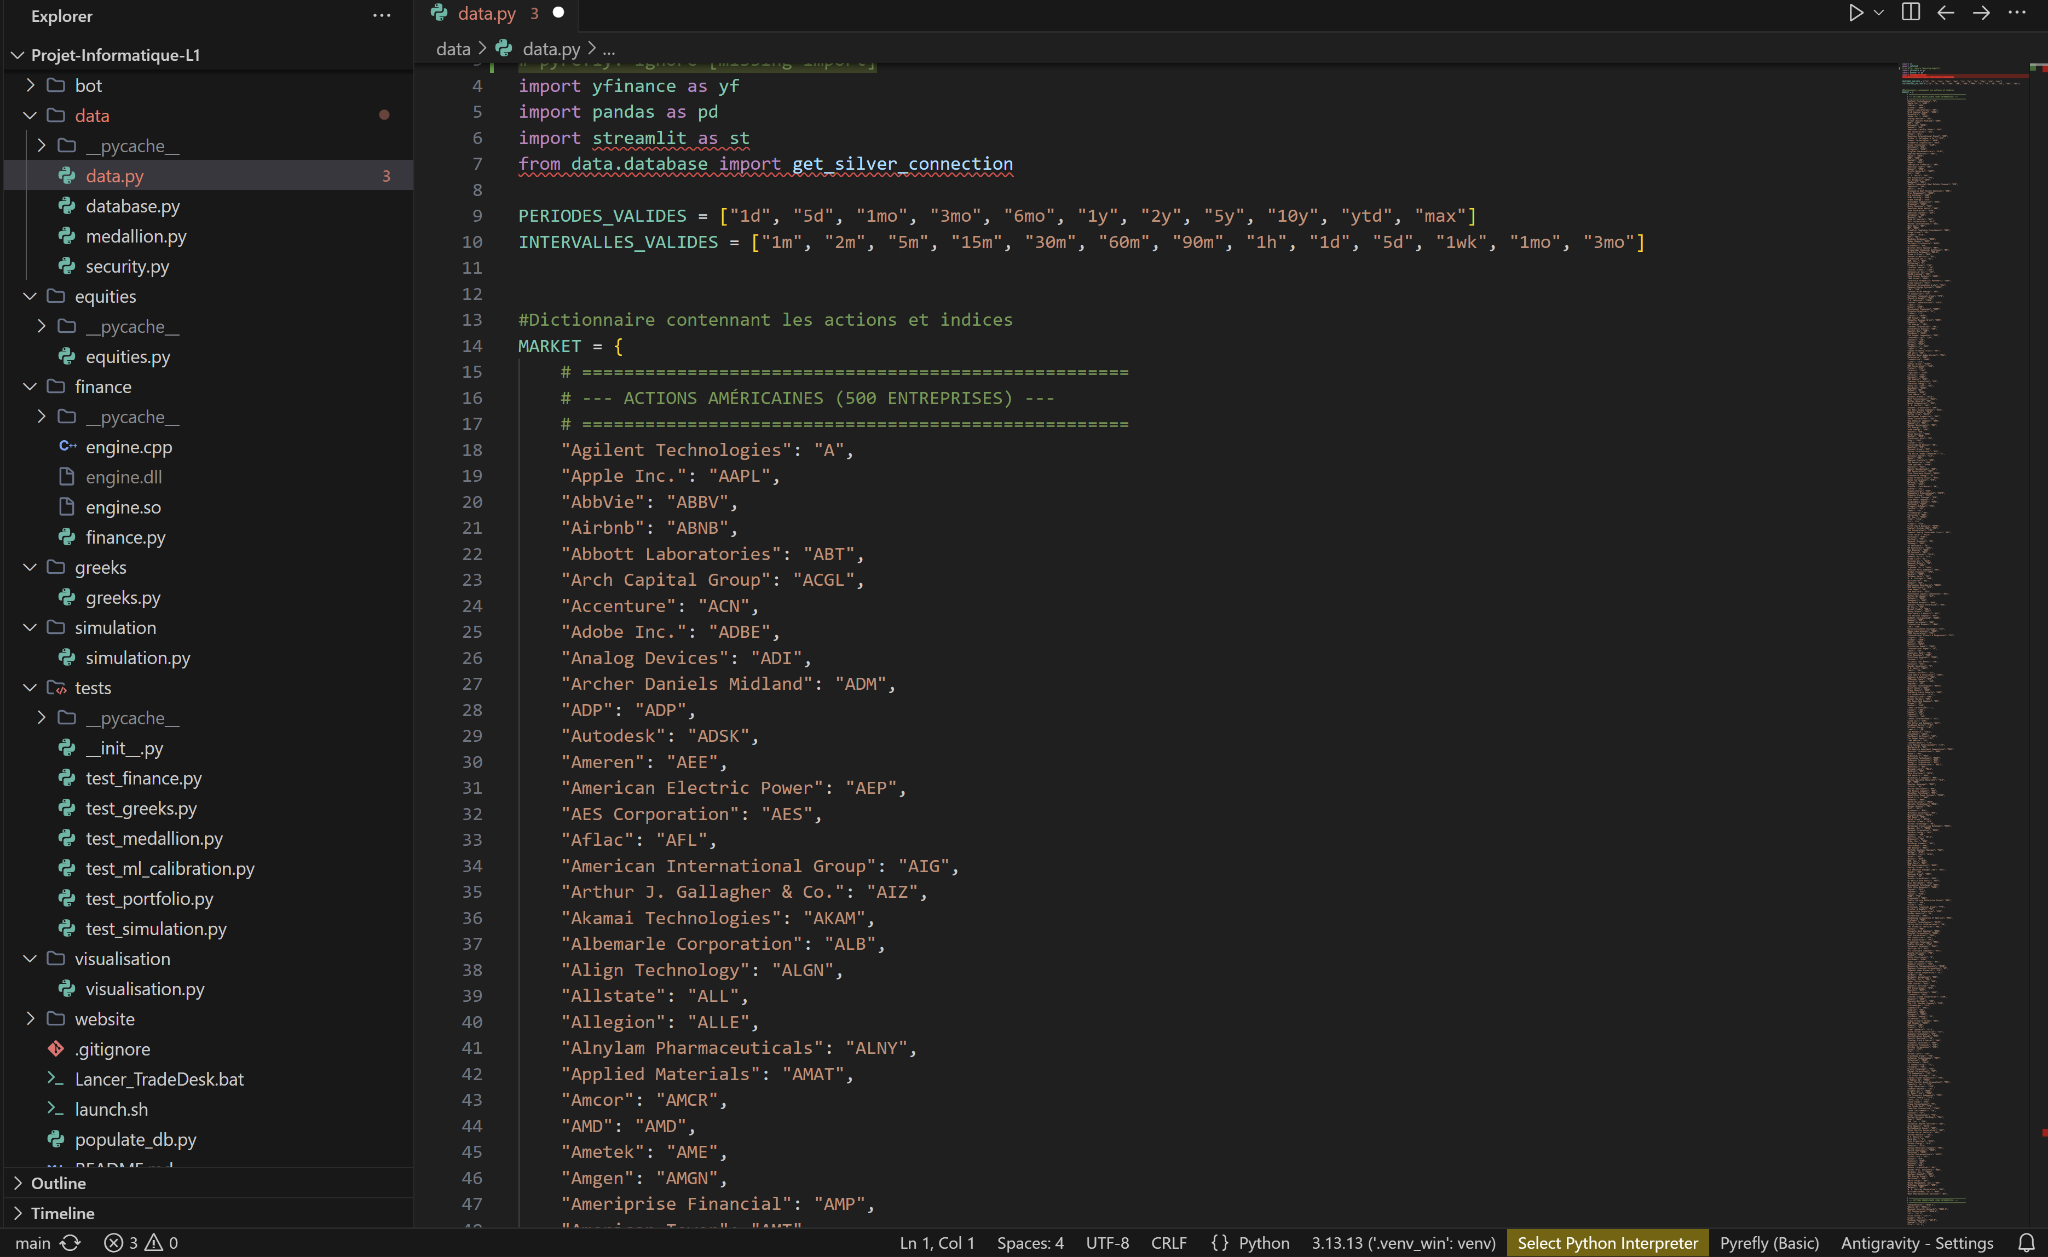
\includegraphics[width=\linewidth]{./media/image14.png}
 
    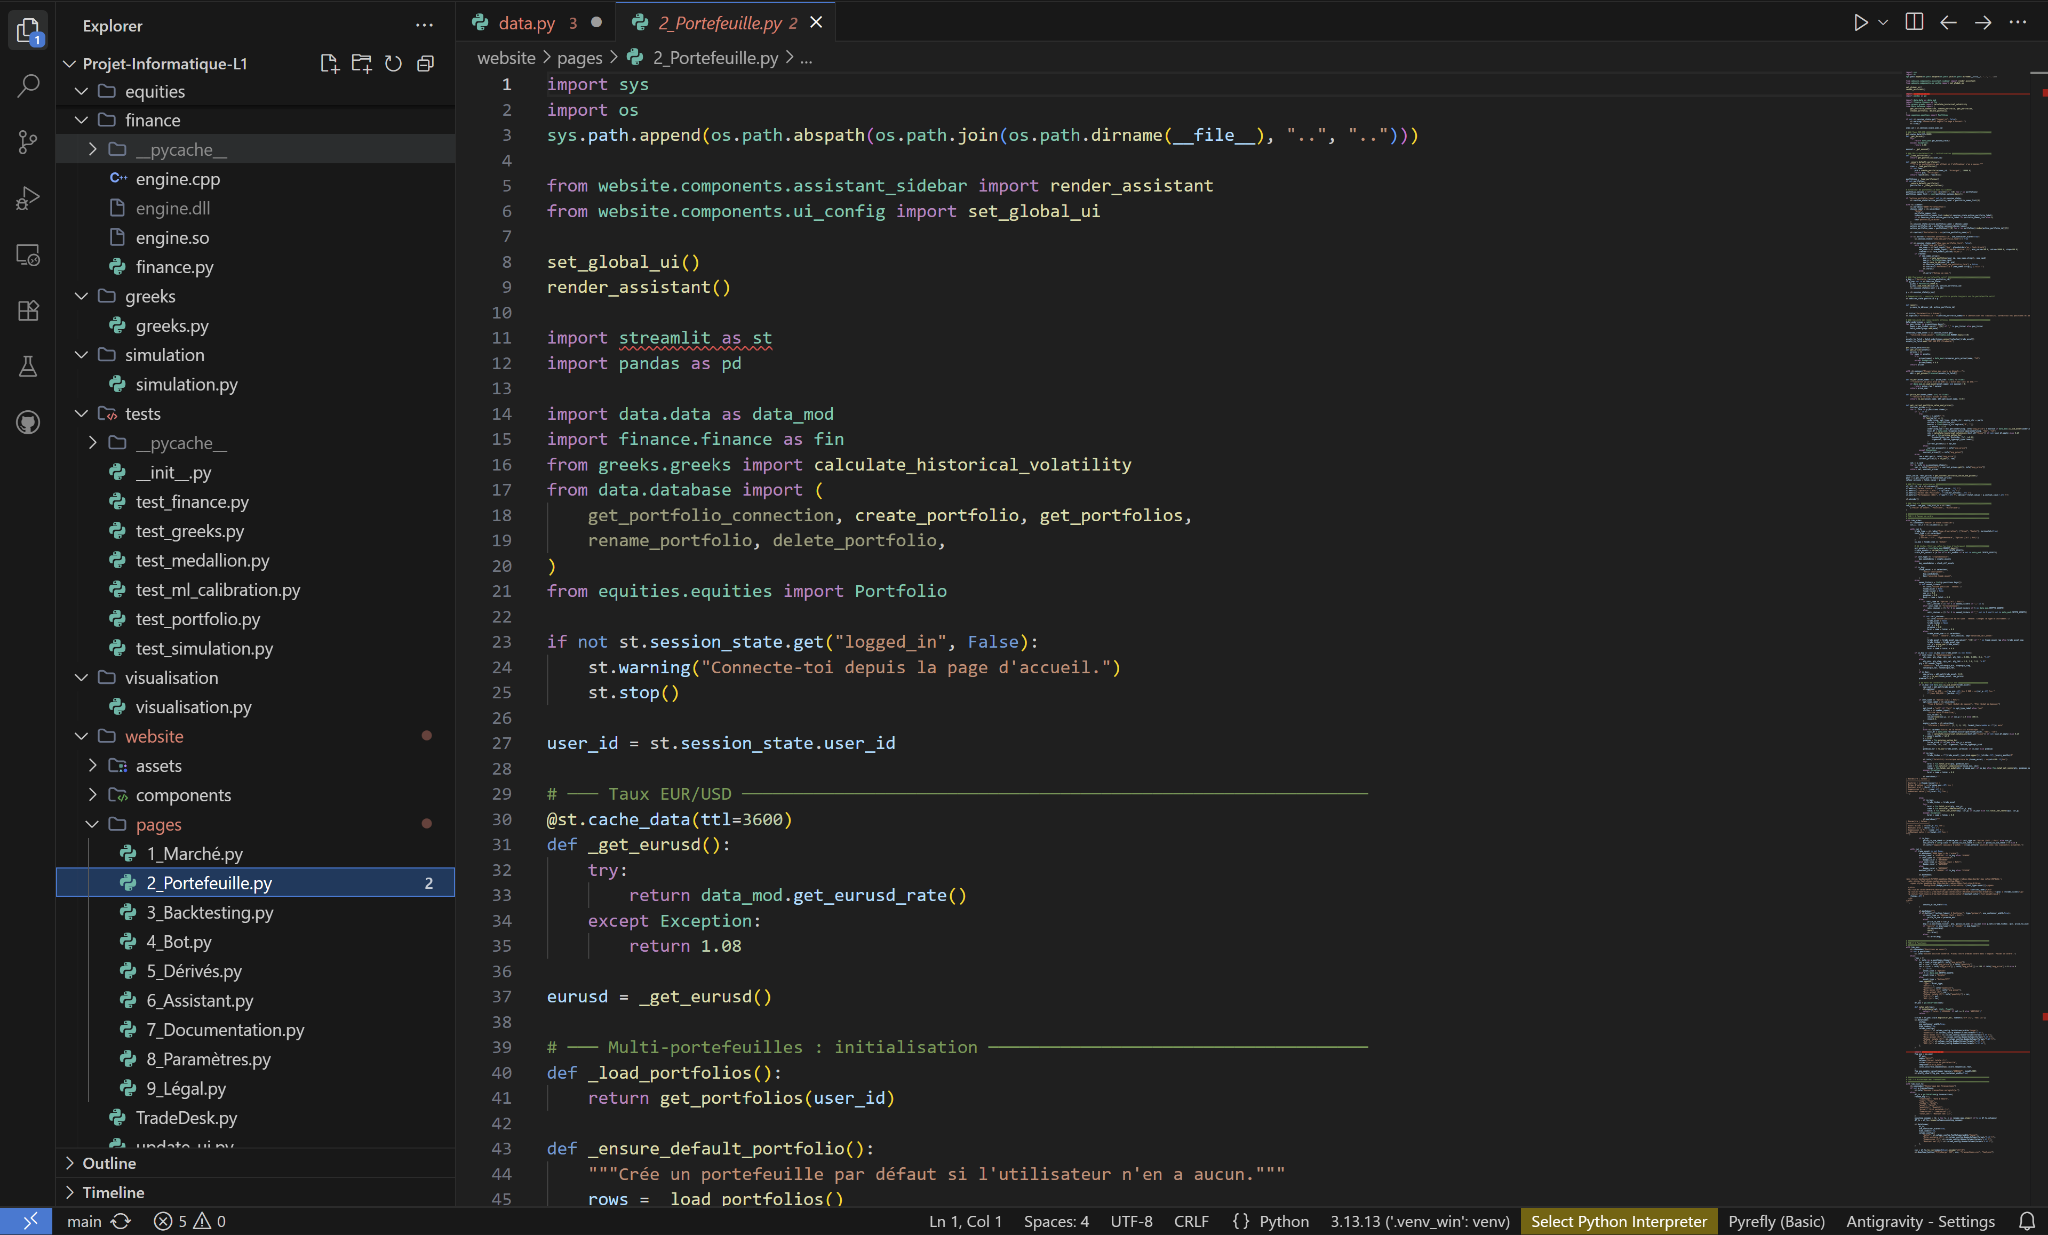
\includegraphics[width=\linewidth]{./media/image1.png}
 
    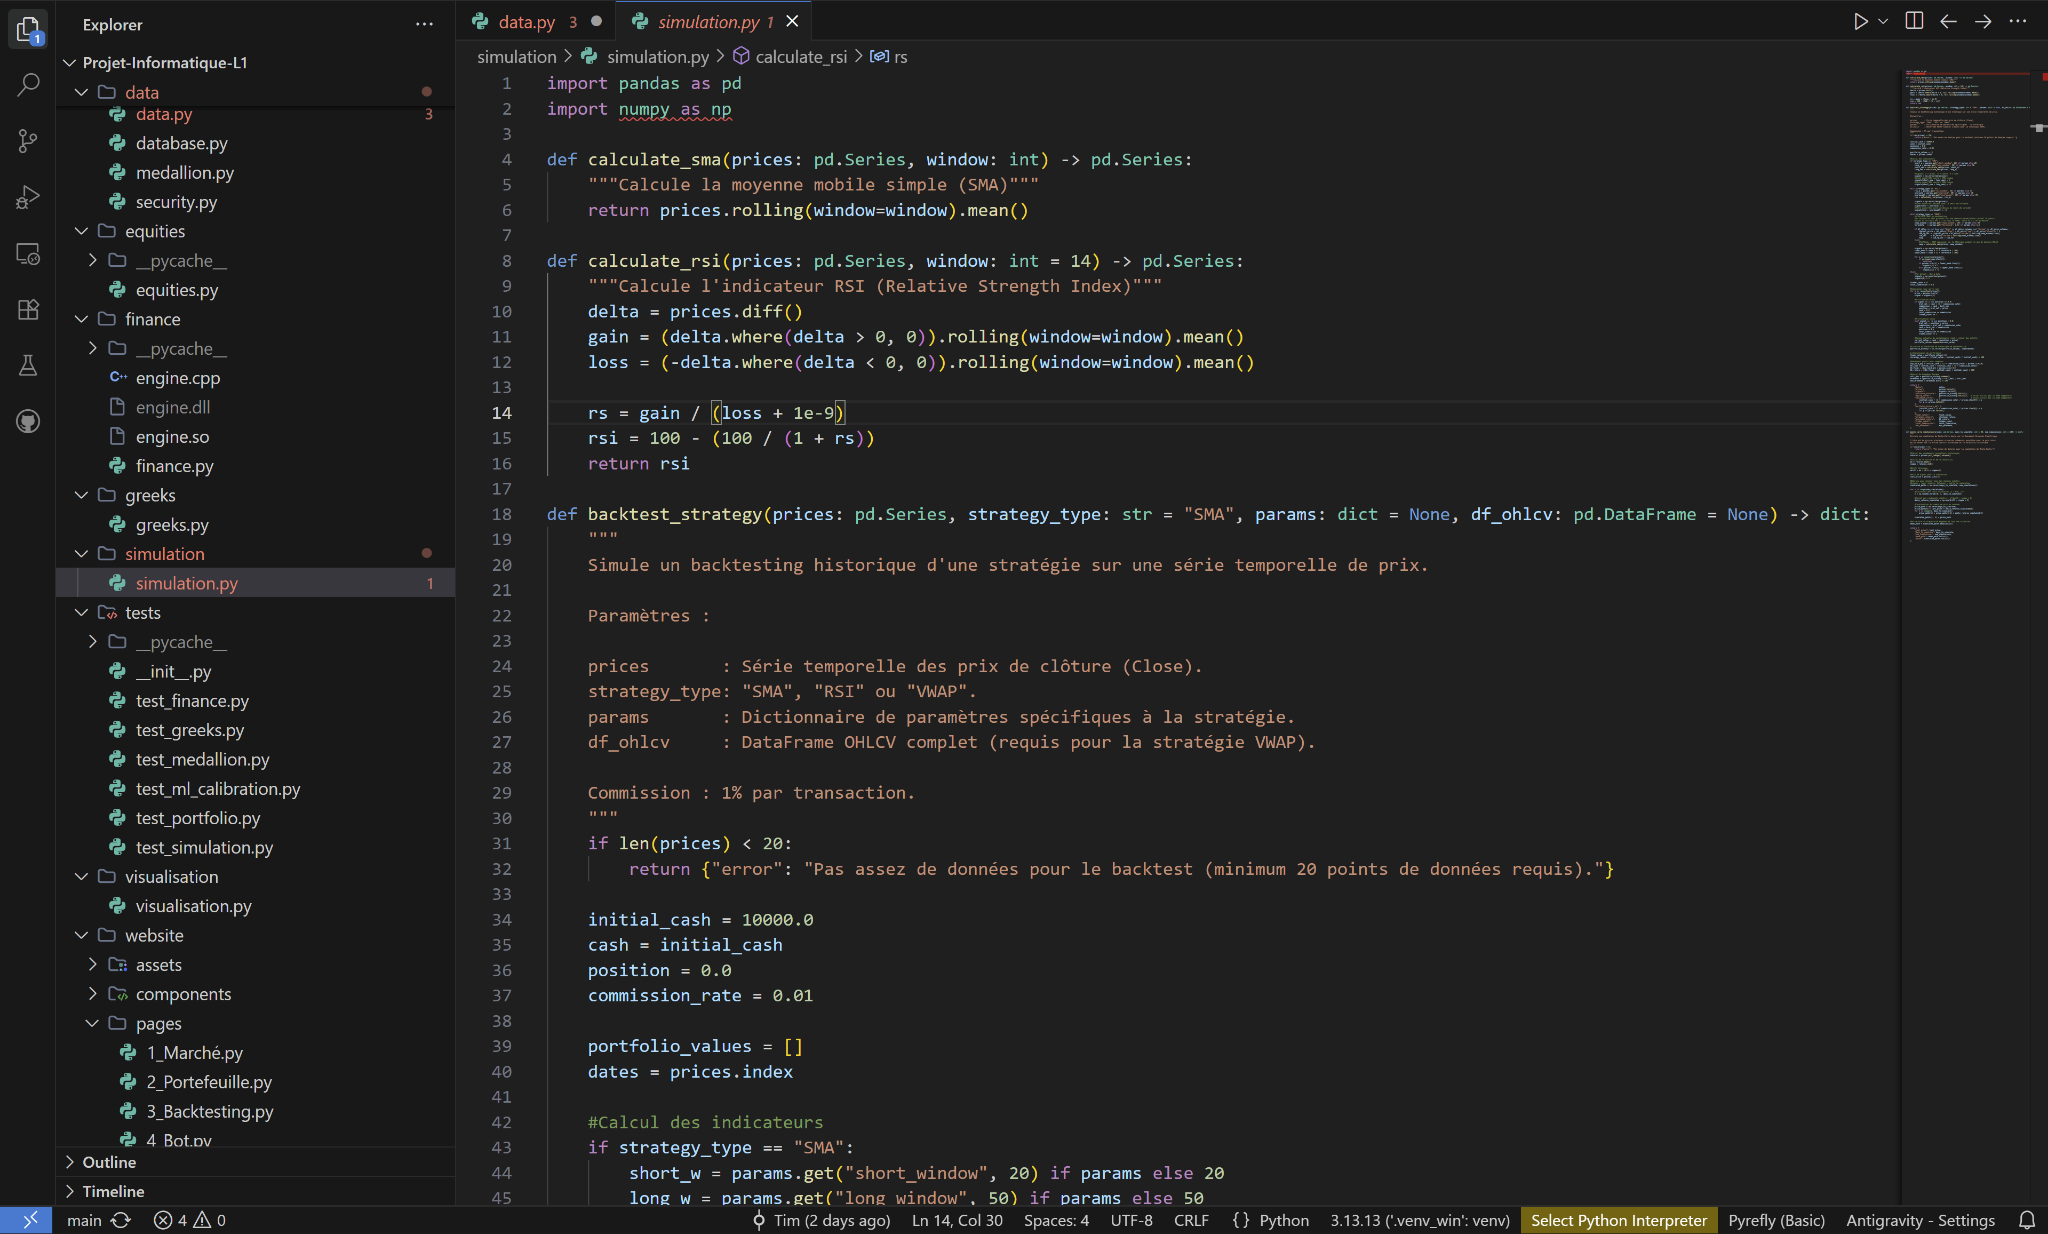
\includegraphics[width=\linewidth]{./media/image25.png}
 
    \textbf{Page 1 --- Page d'accueil et connexion}
 
    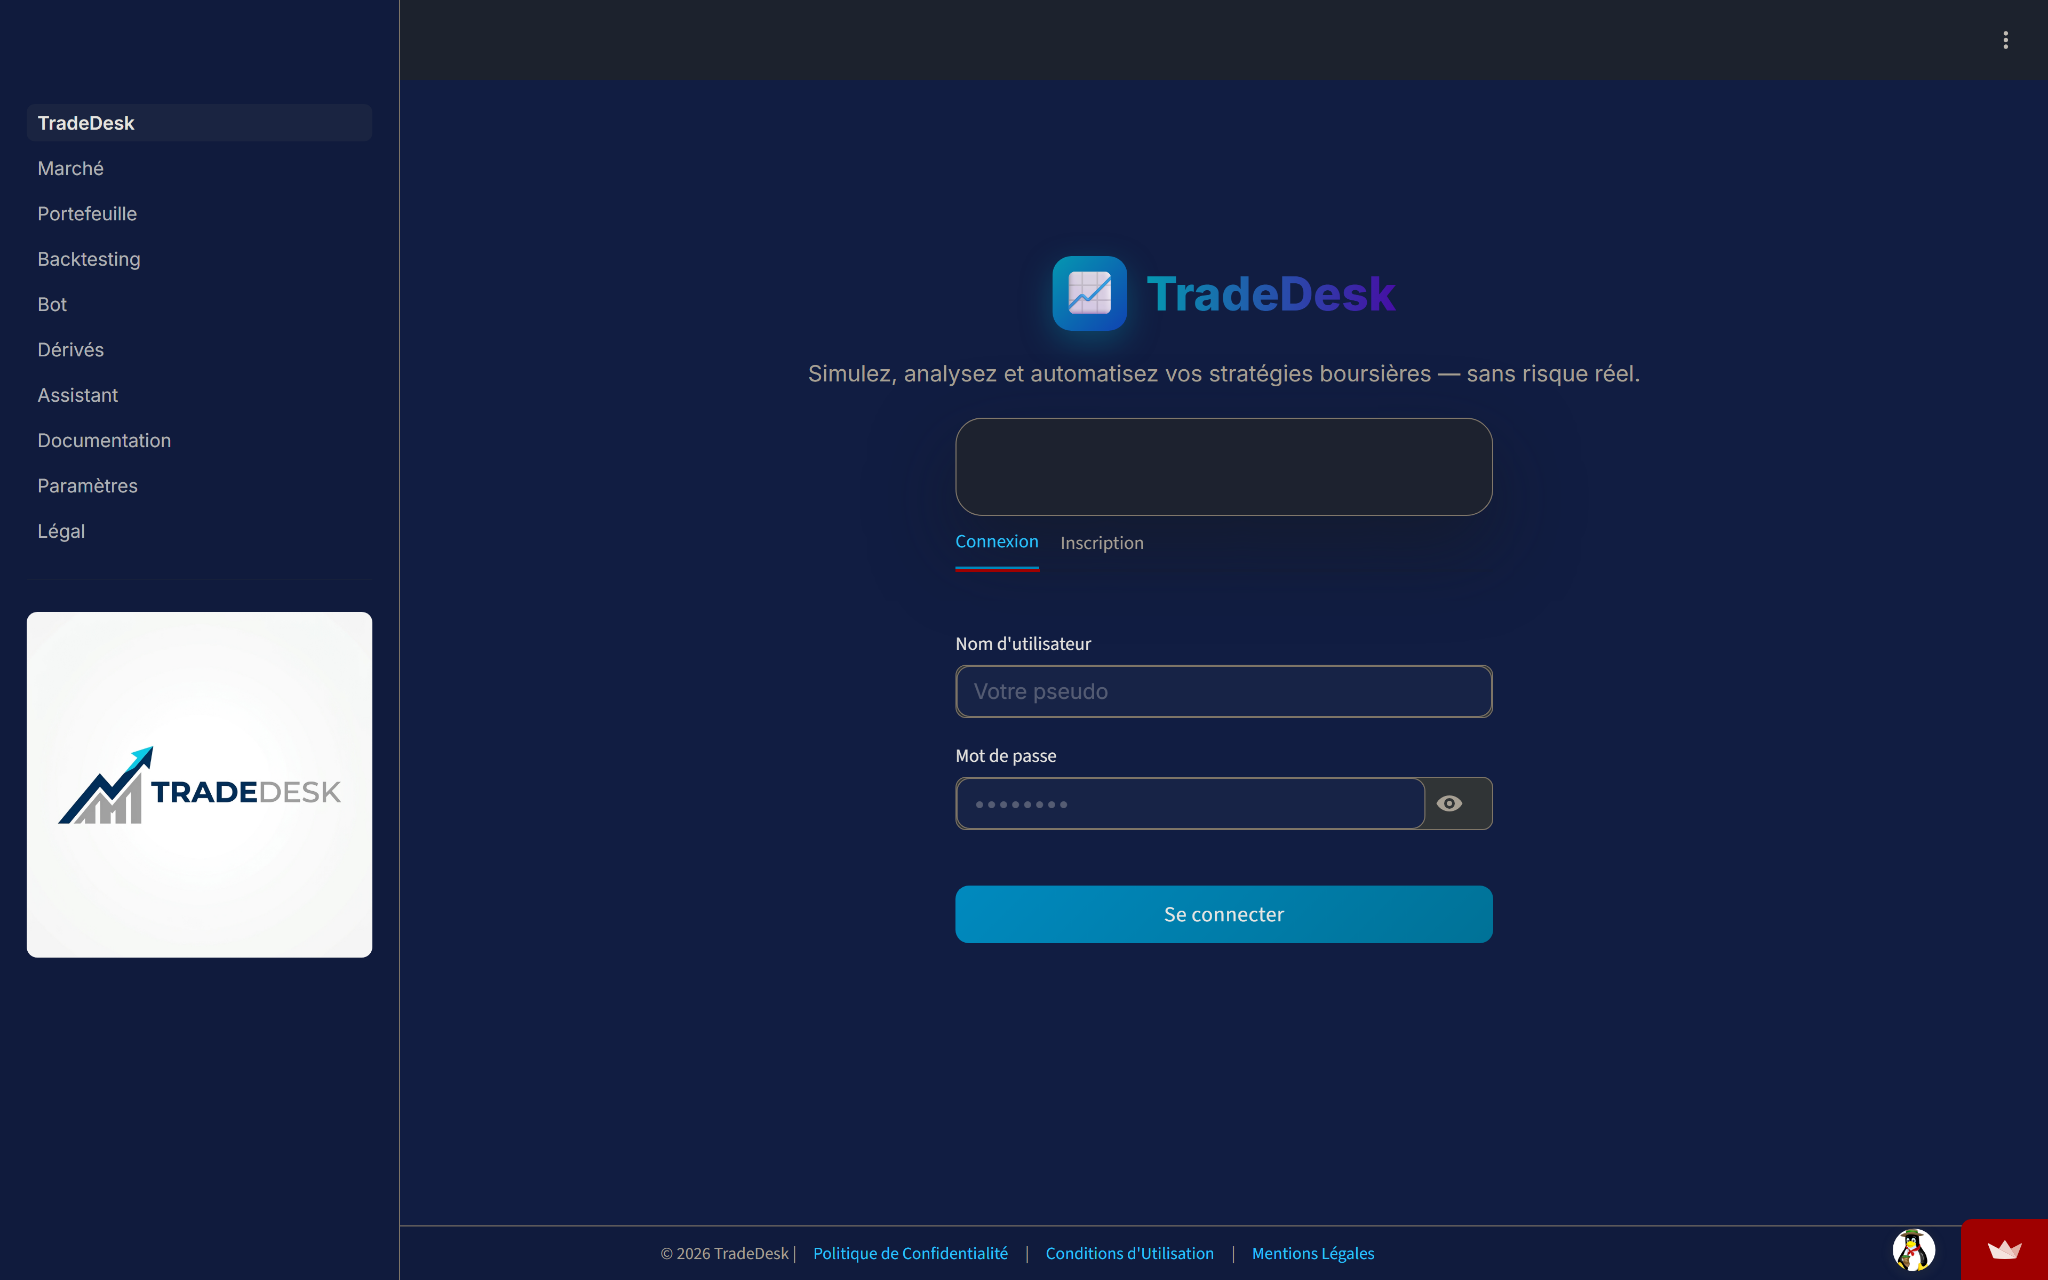
\includegraphics[width=\linewidth]{./media/image18.png}
 
    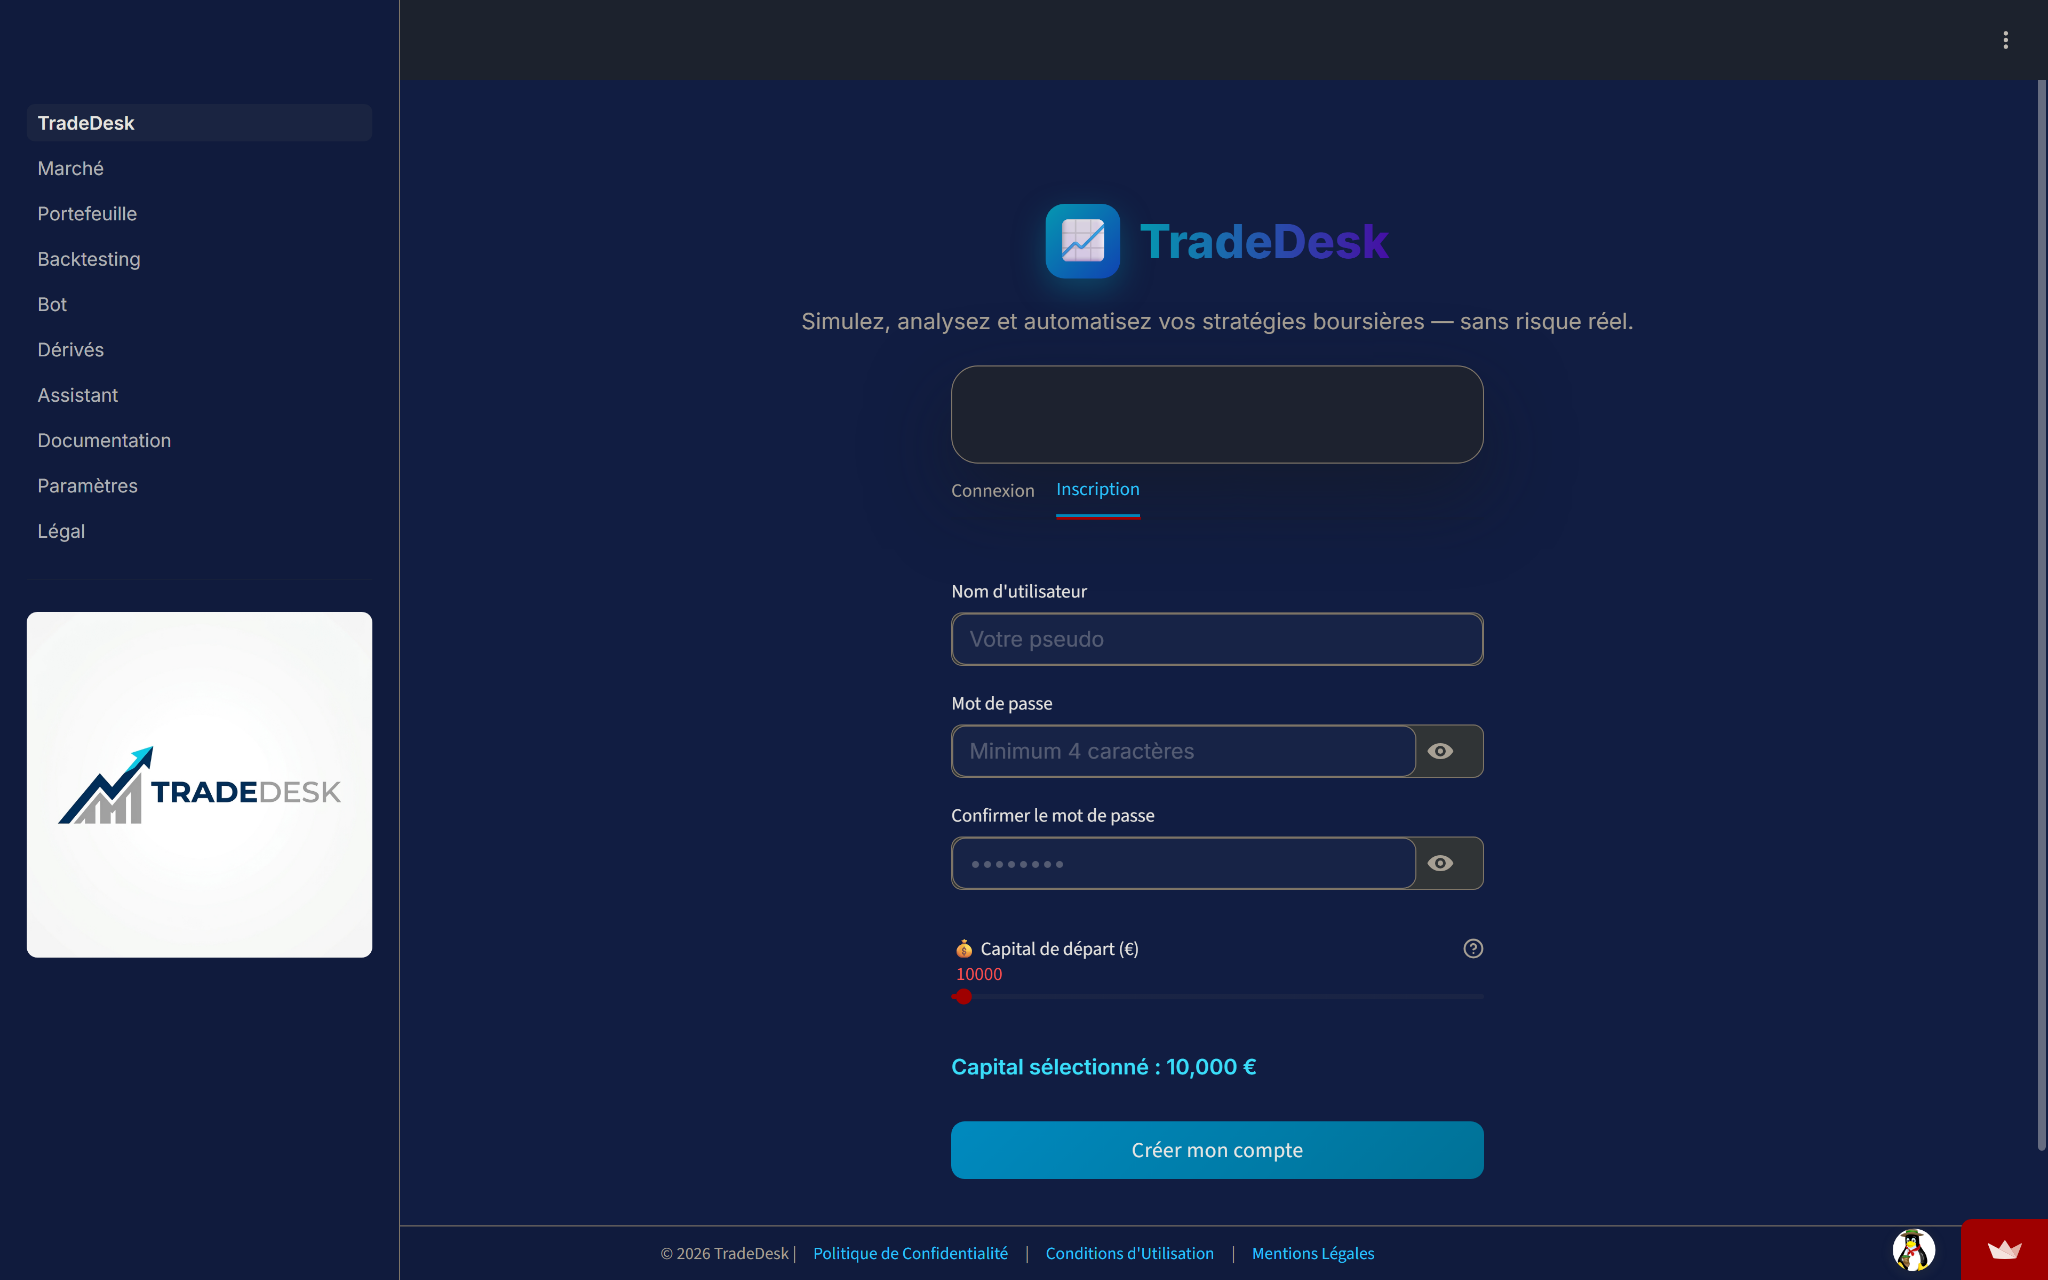
\includegraphics[width=\linewidth]{./media/image12.png}
 
    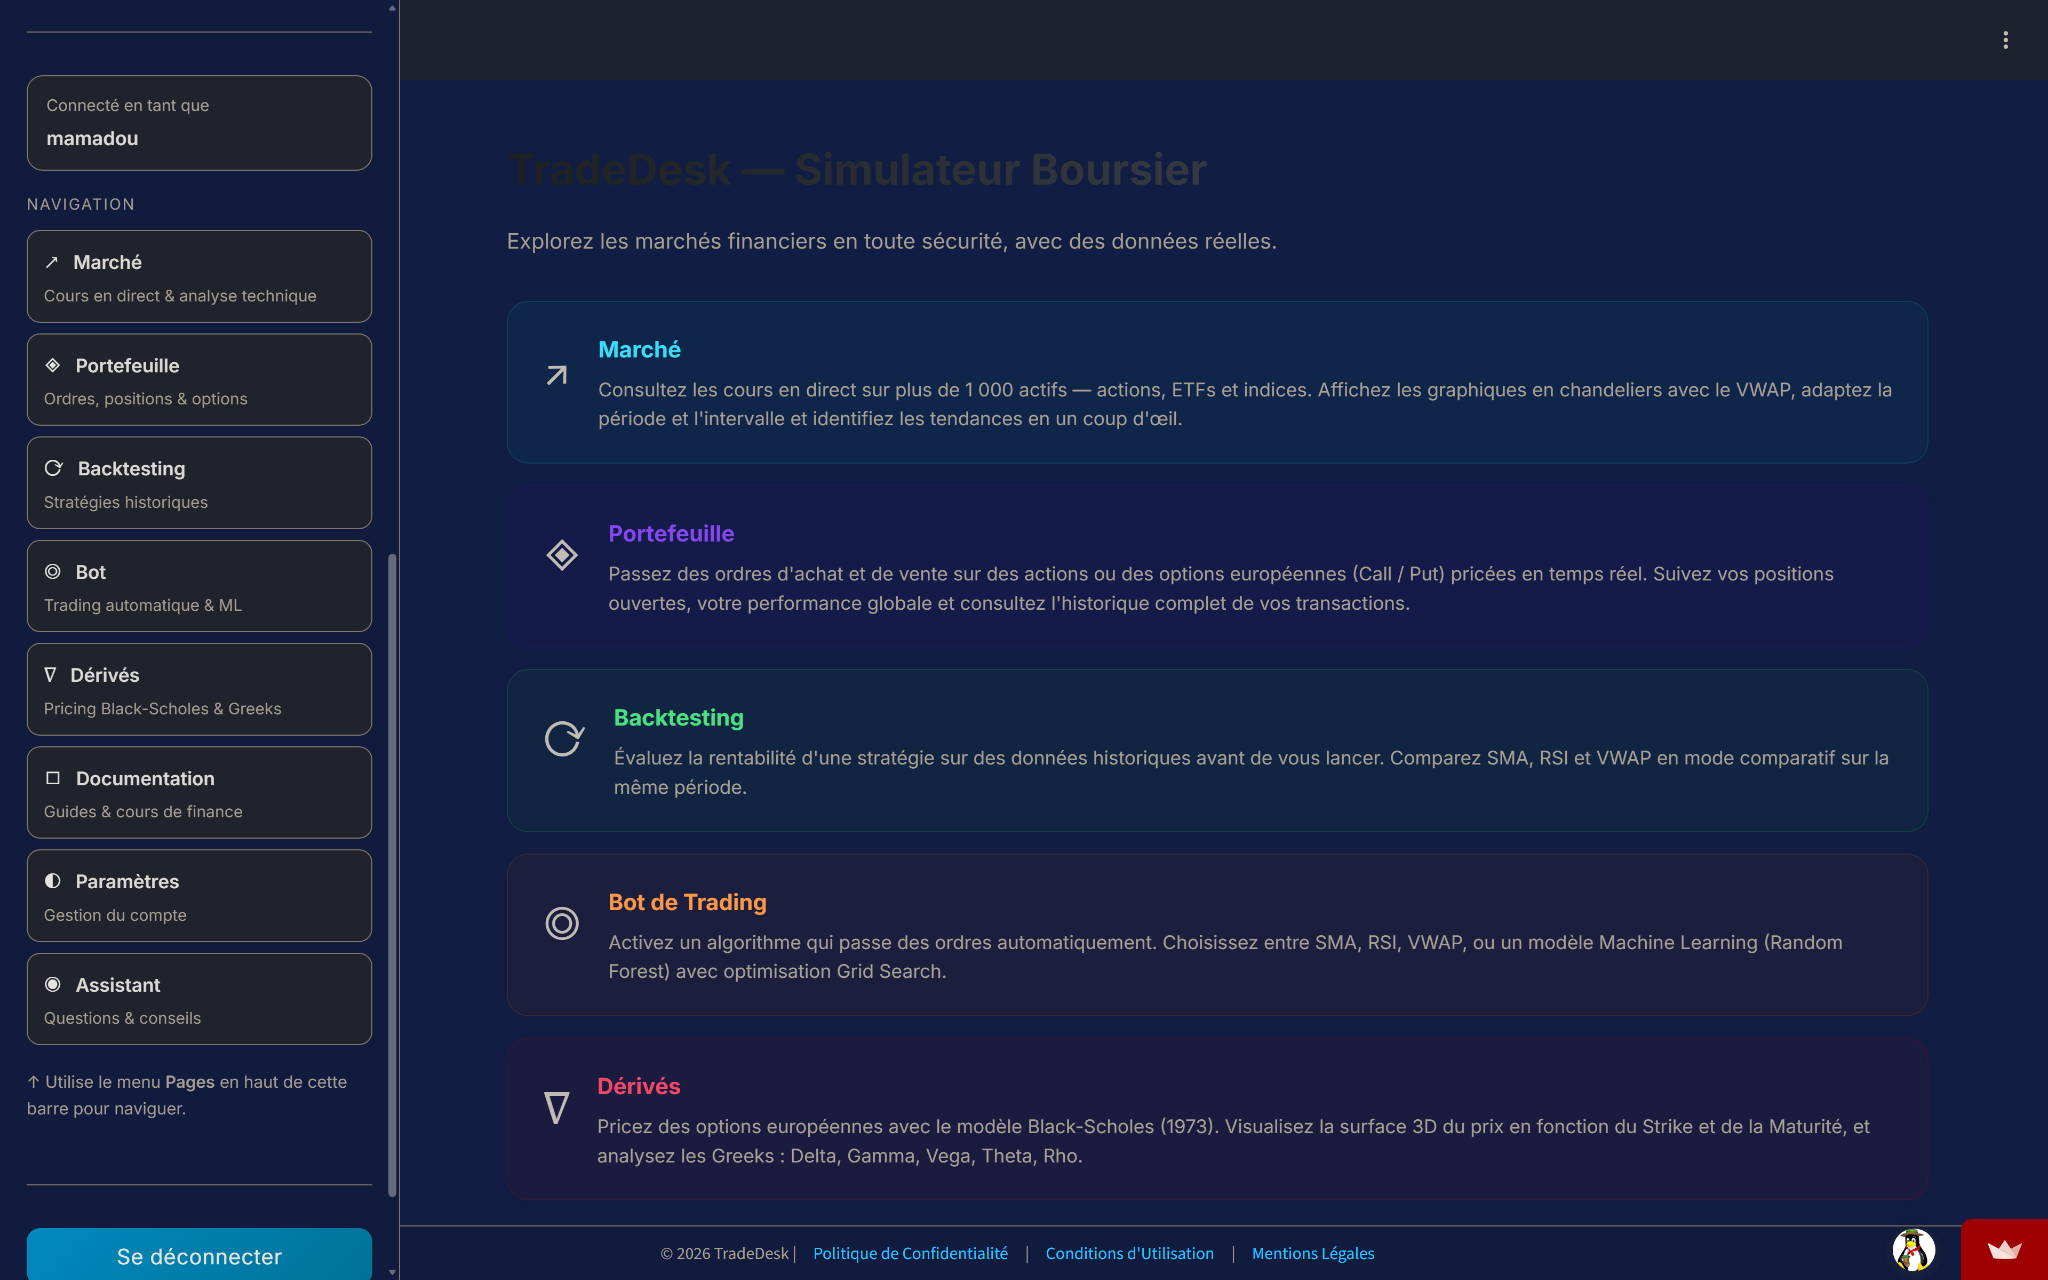
\includegraphics[width=\linewidth]{./media/image17.png}
 
    \textbf{Page 2 --- Analyse de marché (onglet Temps Réel)}
 
    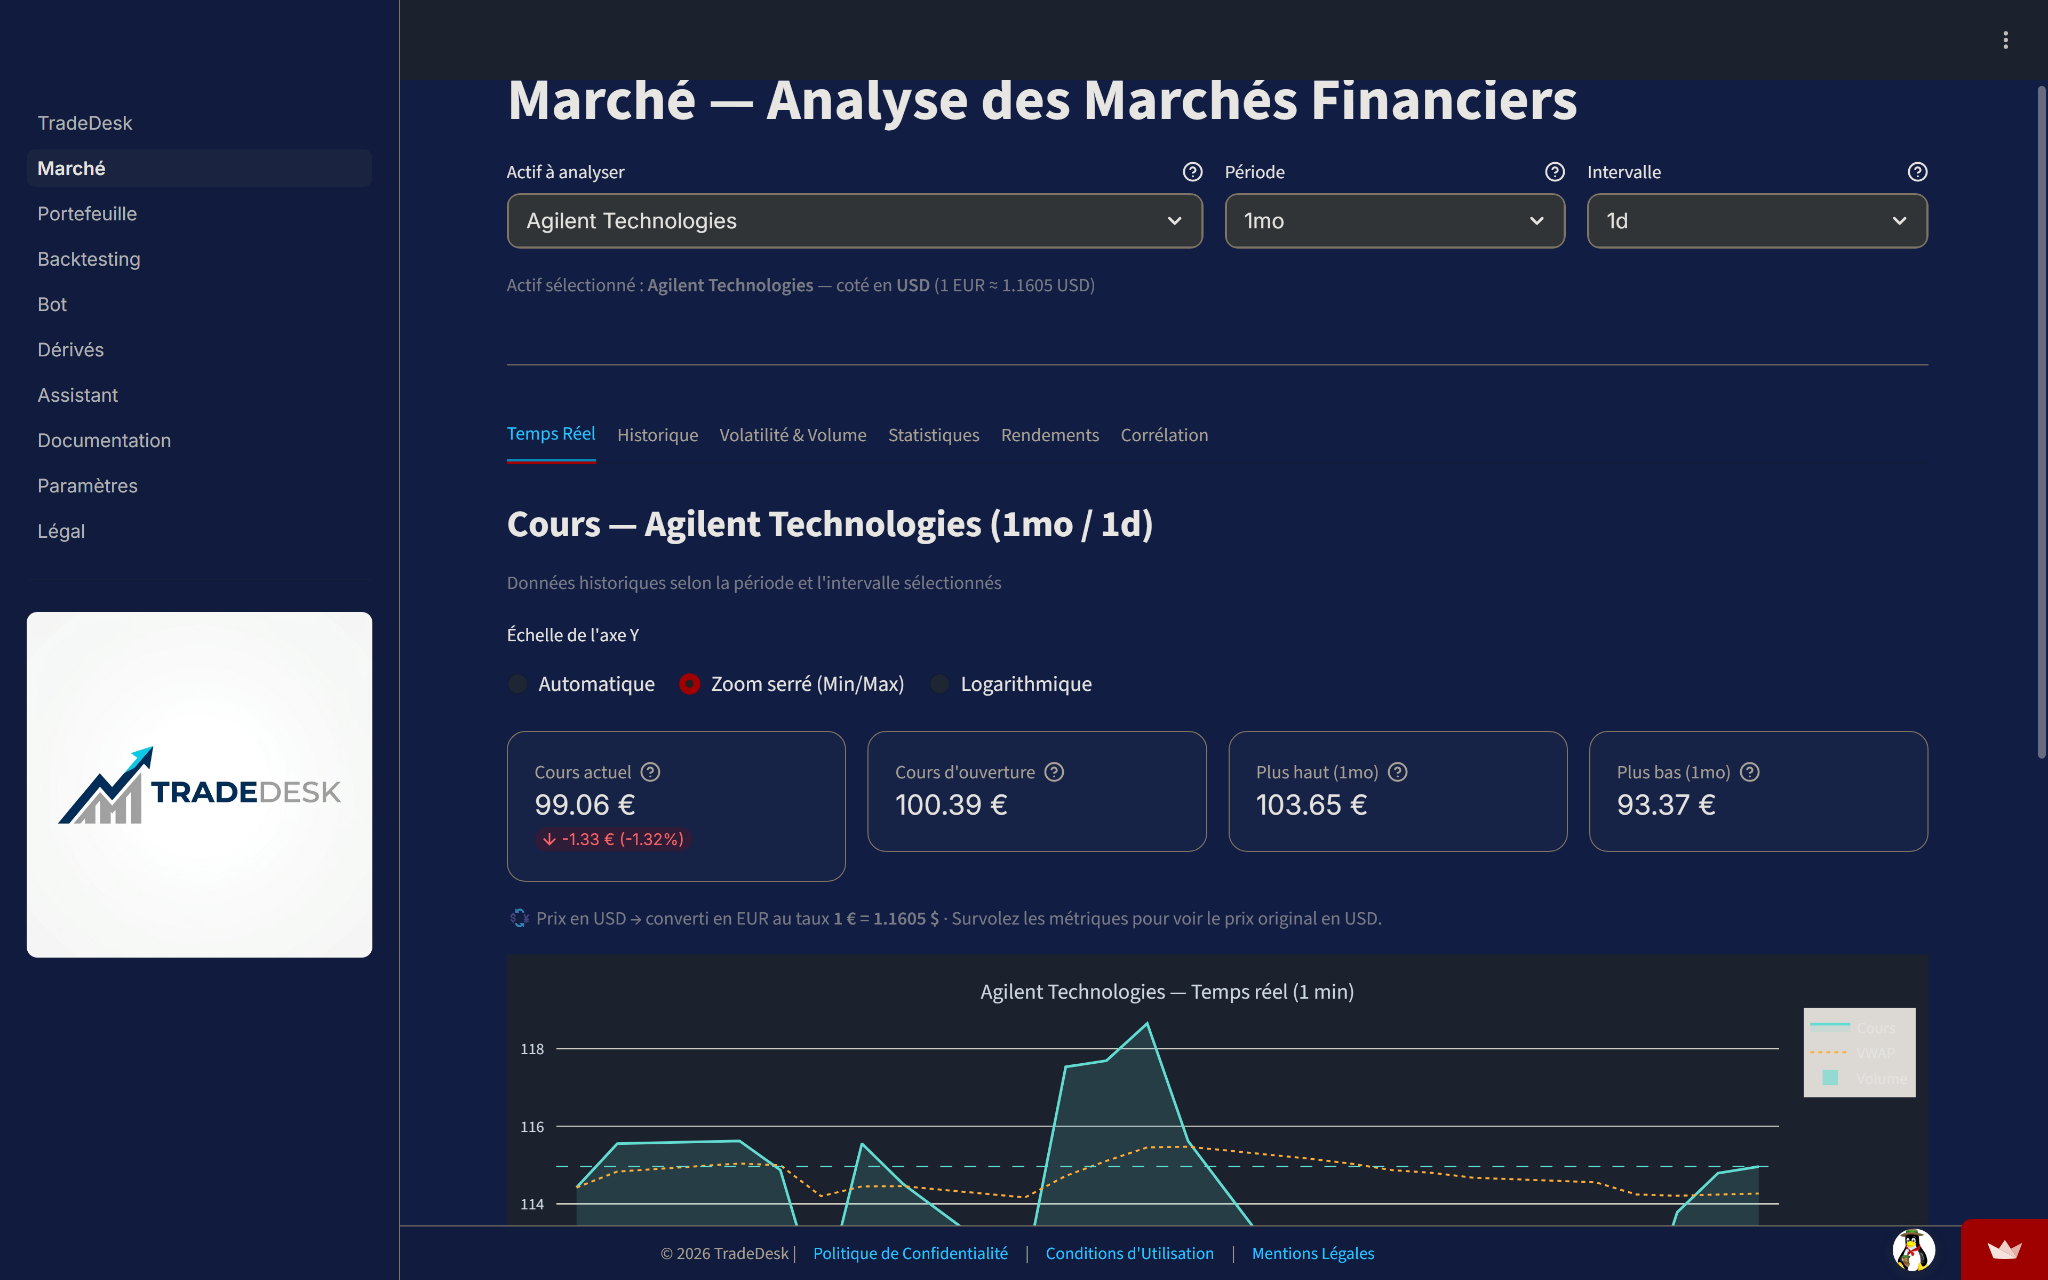
\includegraphics[width=\linewidth]{./media/image21.png}
 
    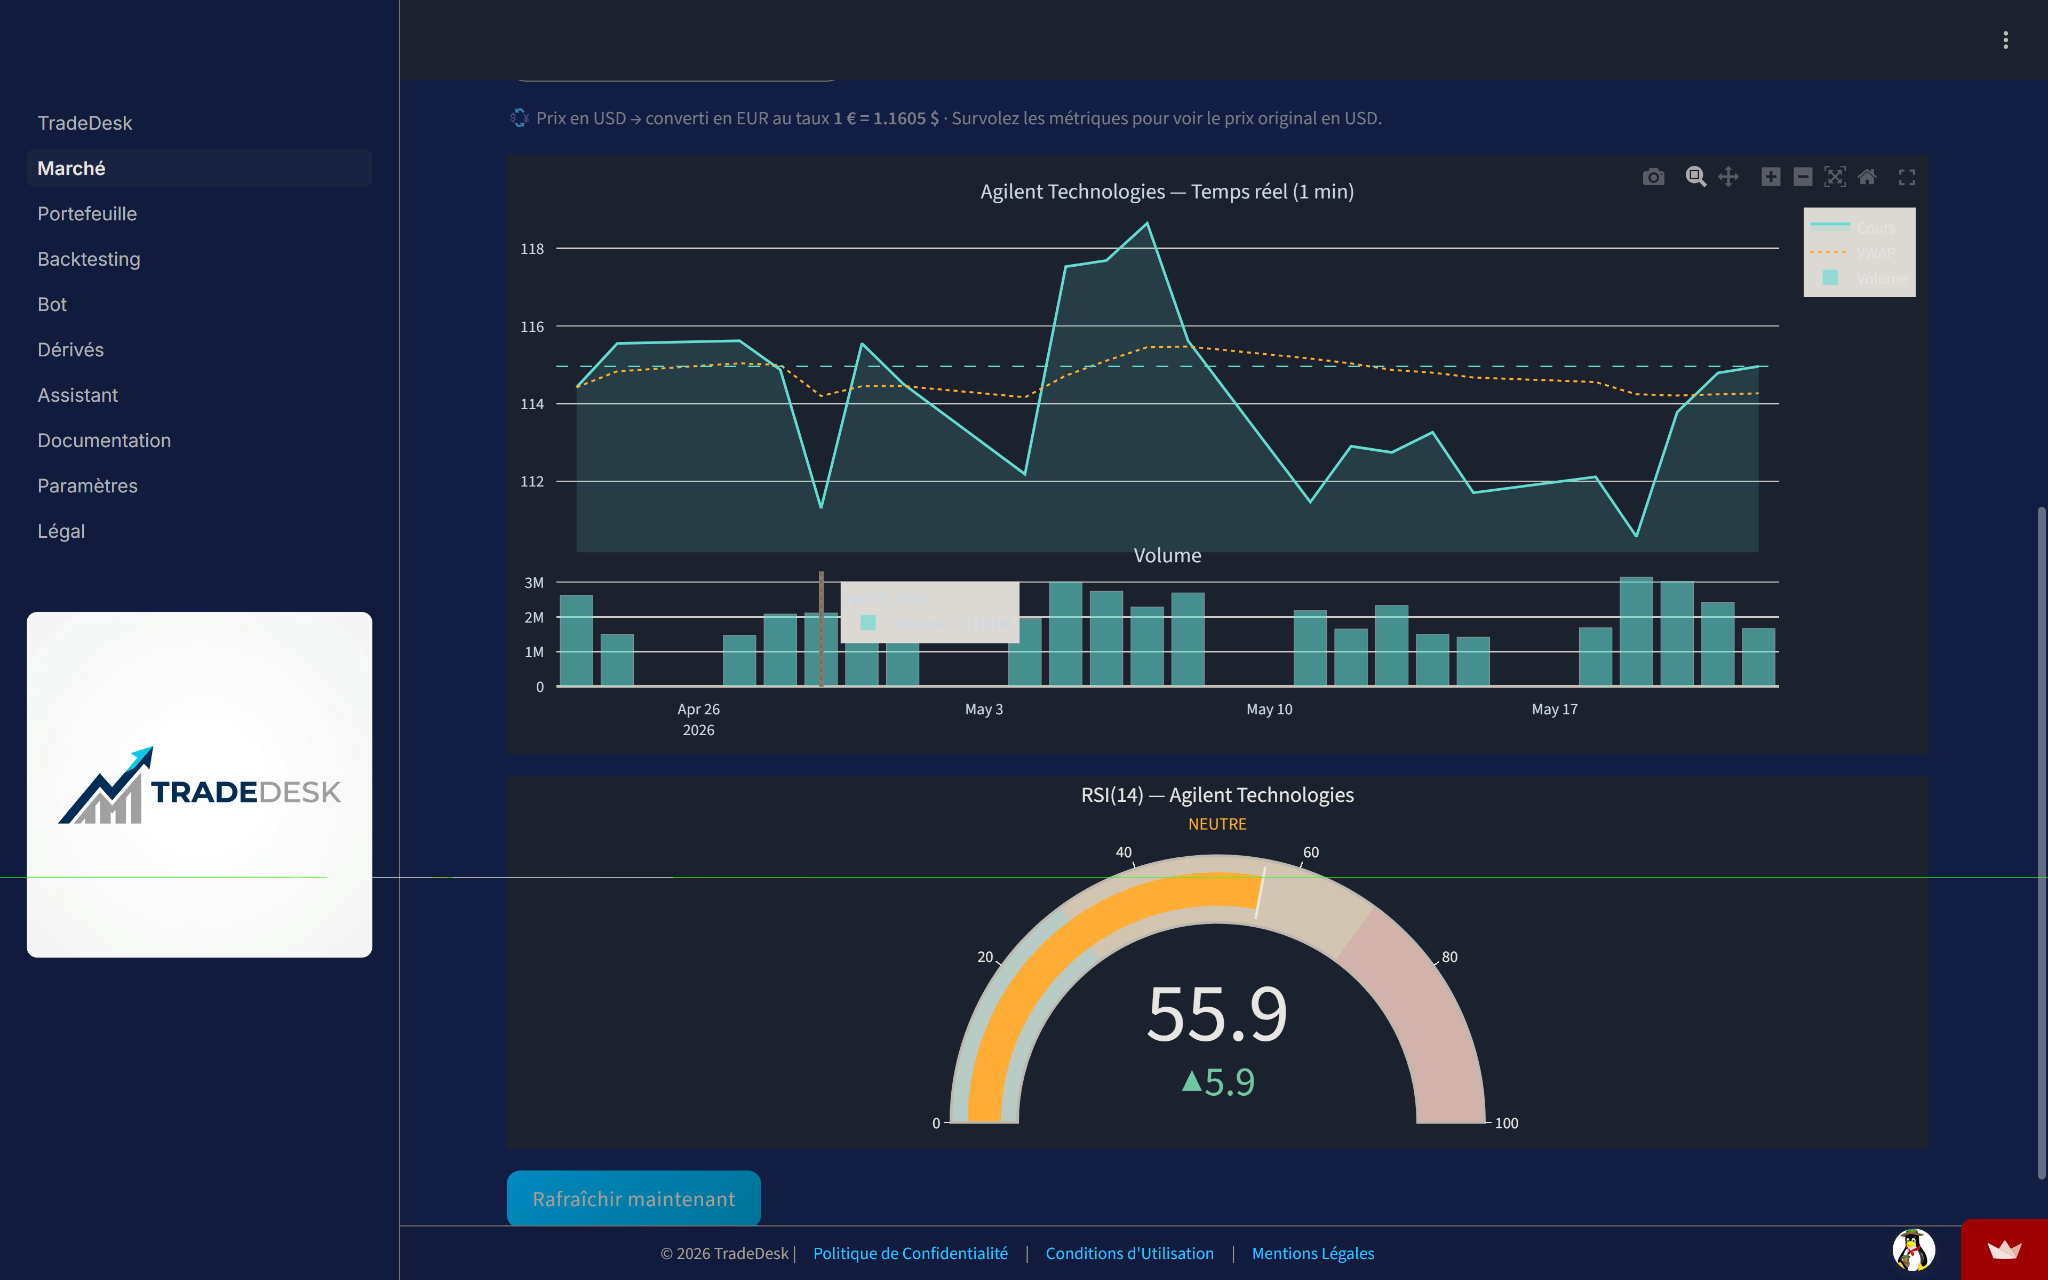
\includegraphics[width=\linewidth]{./media/image26.png}
 
    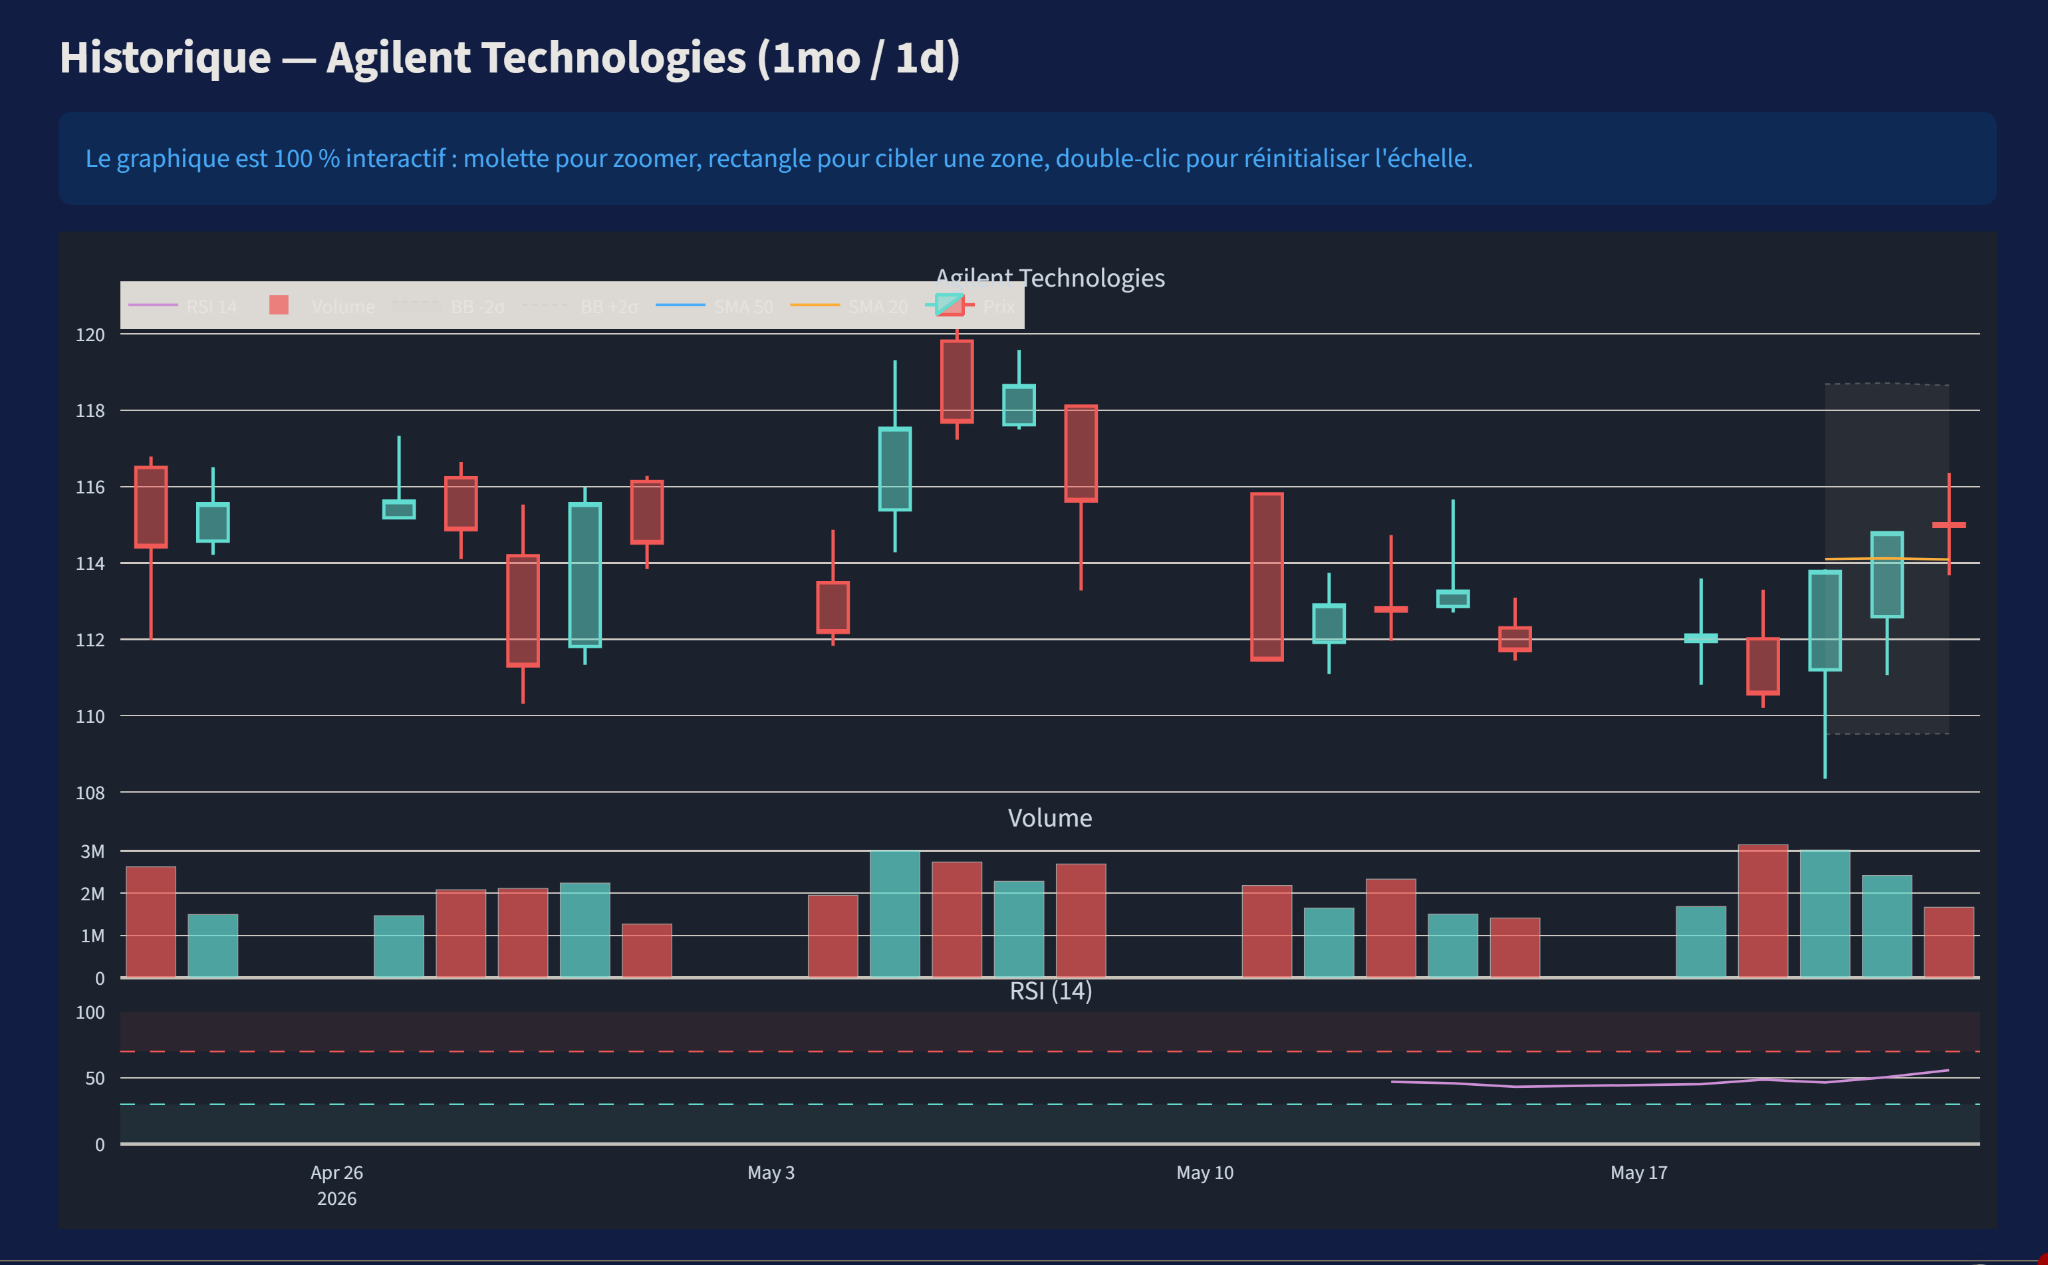
\includegraphics[width=\linewidth]{./media/image19.png}
 
    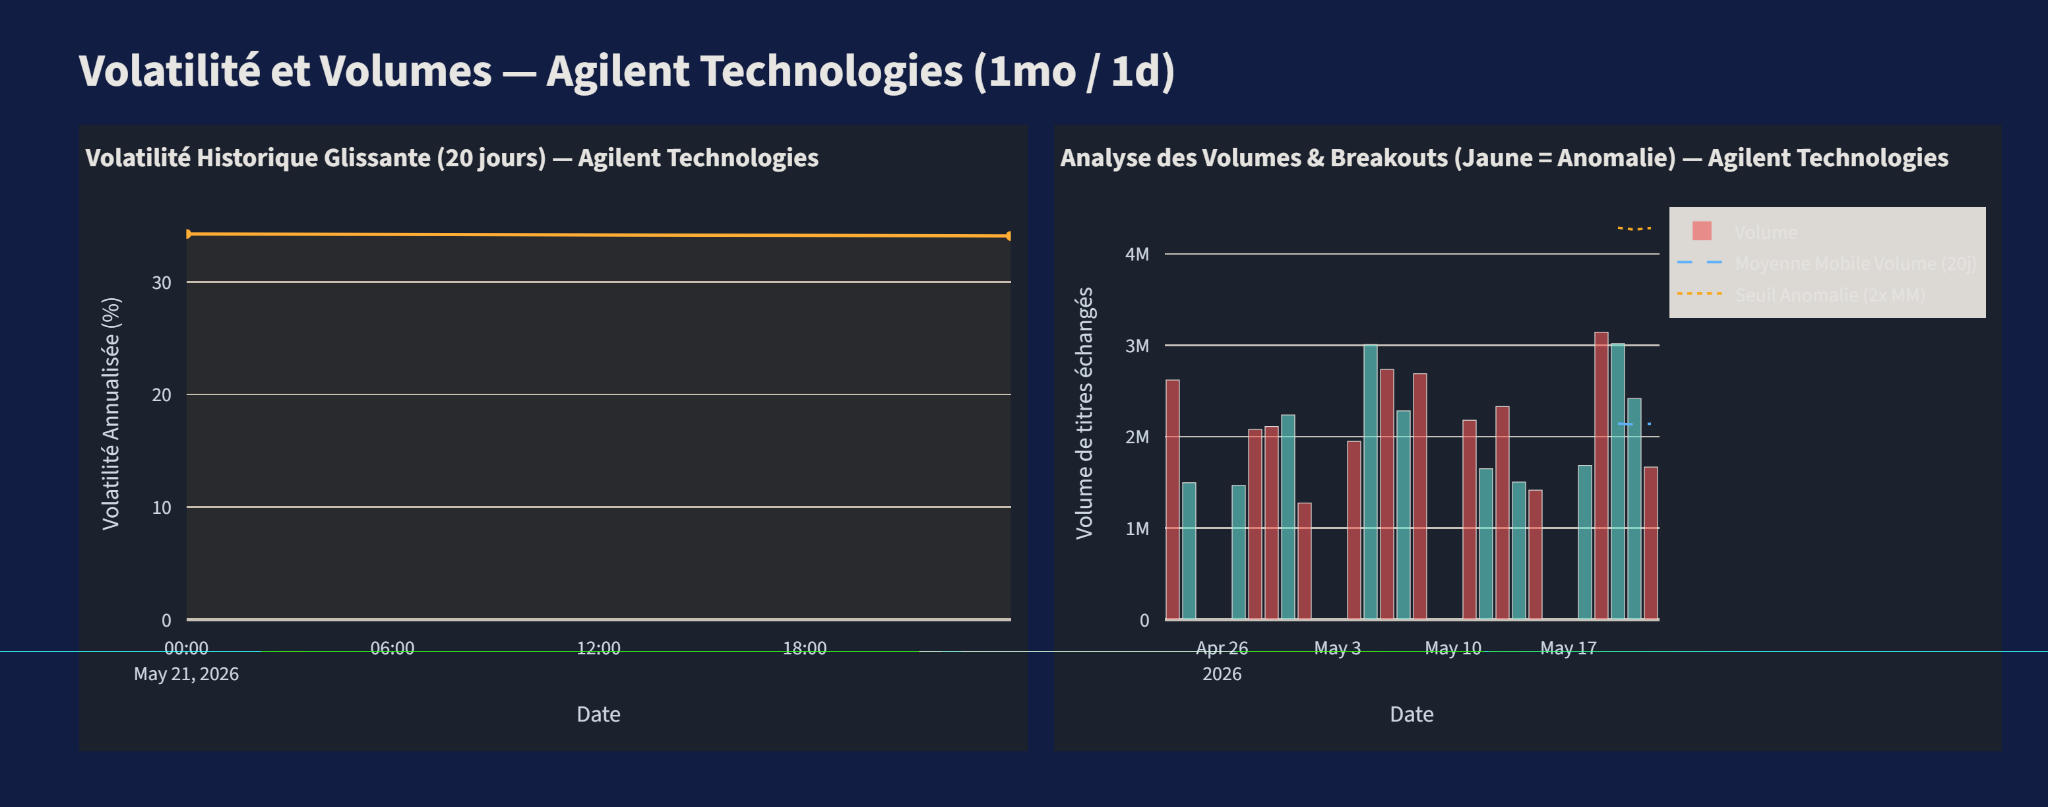
\includegraphics[width=\linewidth]{./media/image24.png}
 
    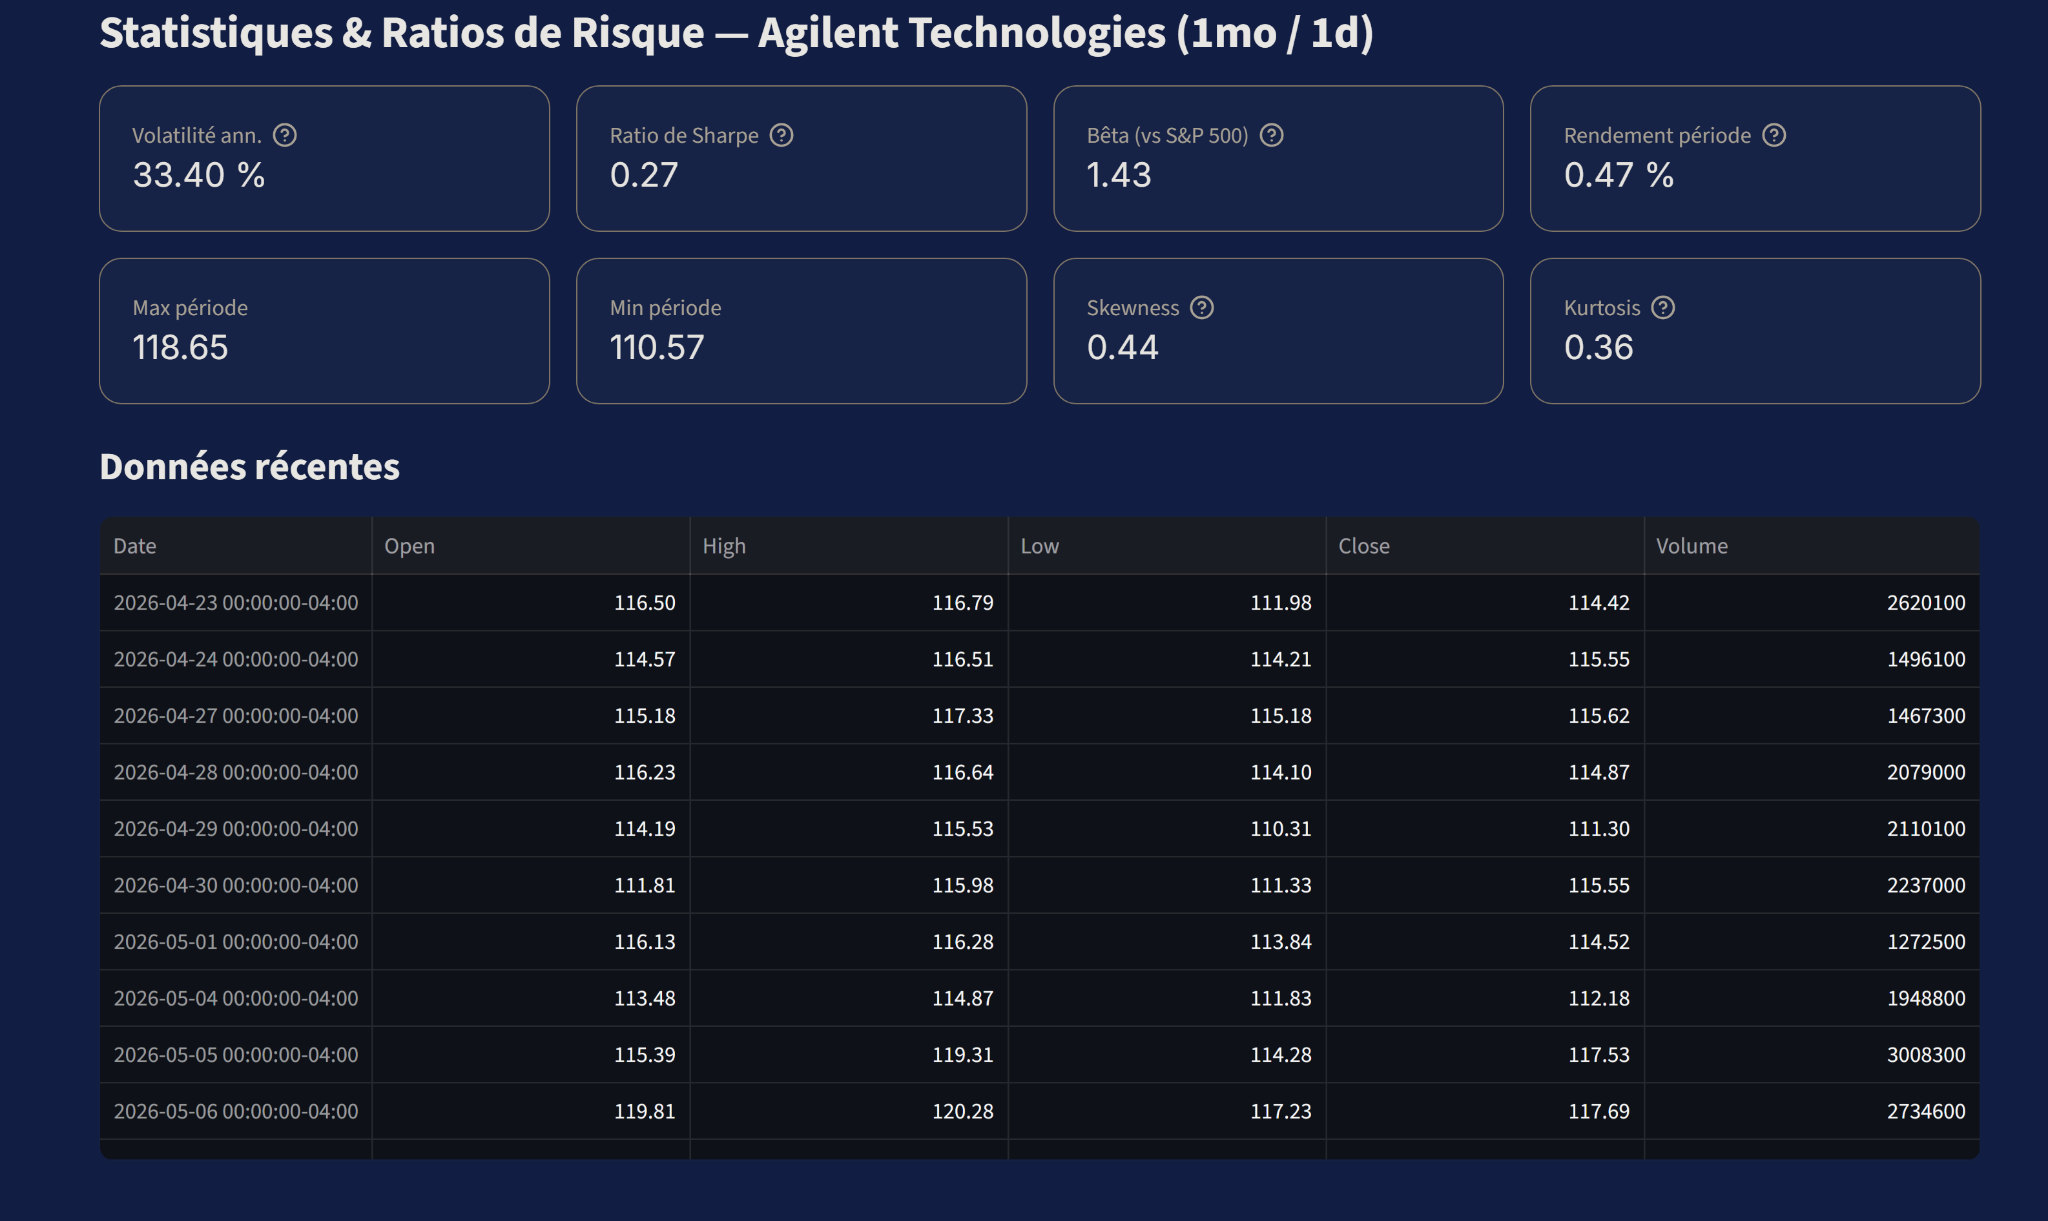
\includegraphics[width=\linewidth]{./media/image9.png}
 
    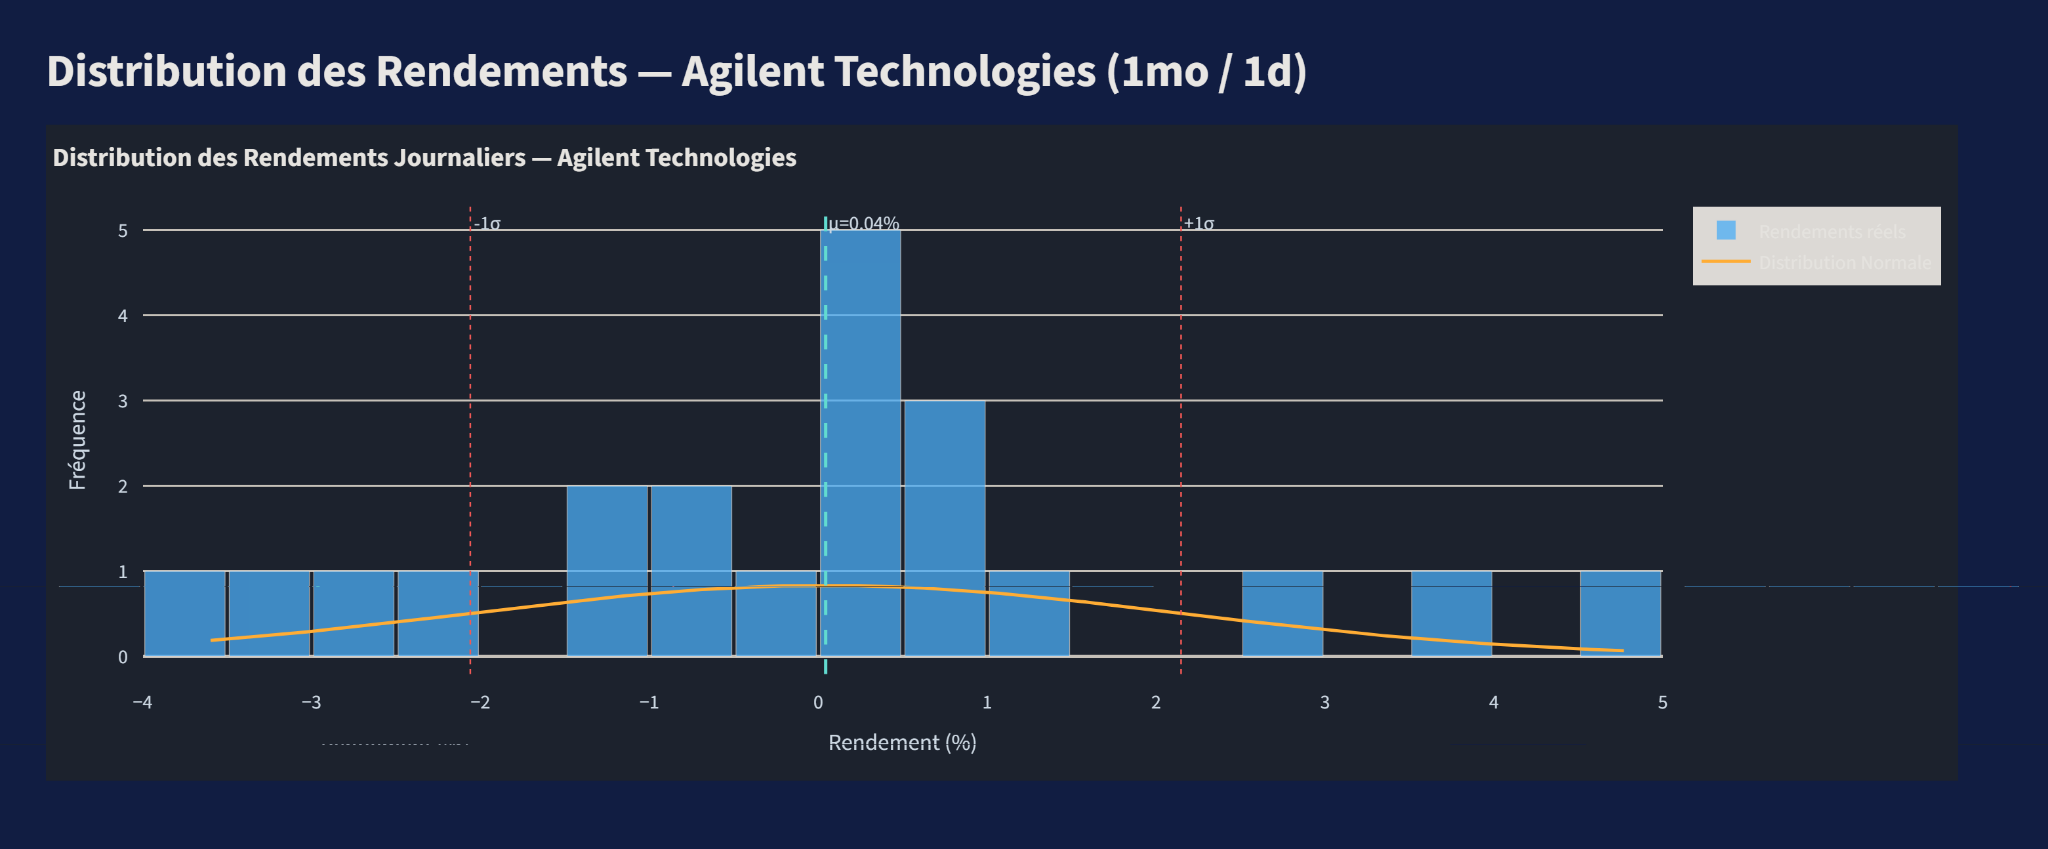
\includegraphics[width=\linewidth]{./media/image10.png}
 
    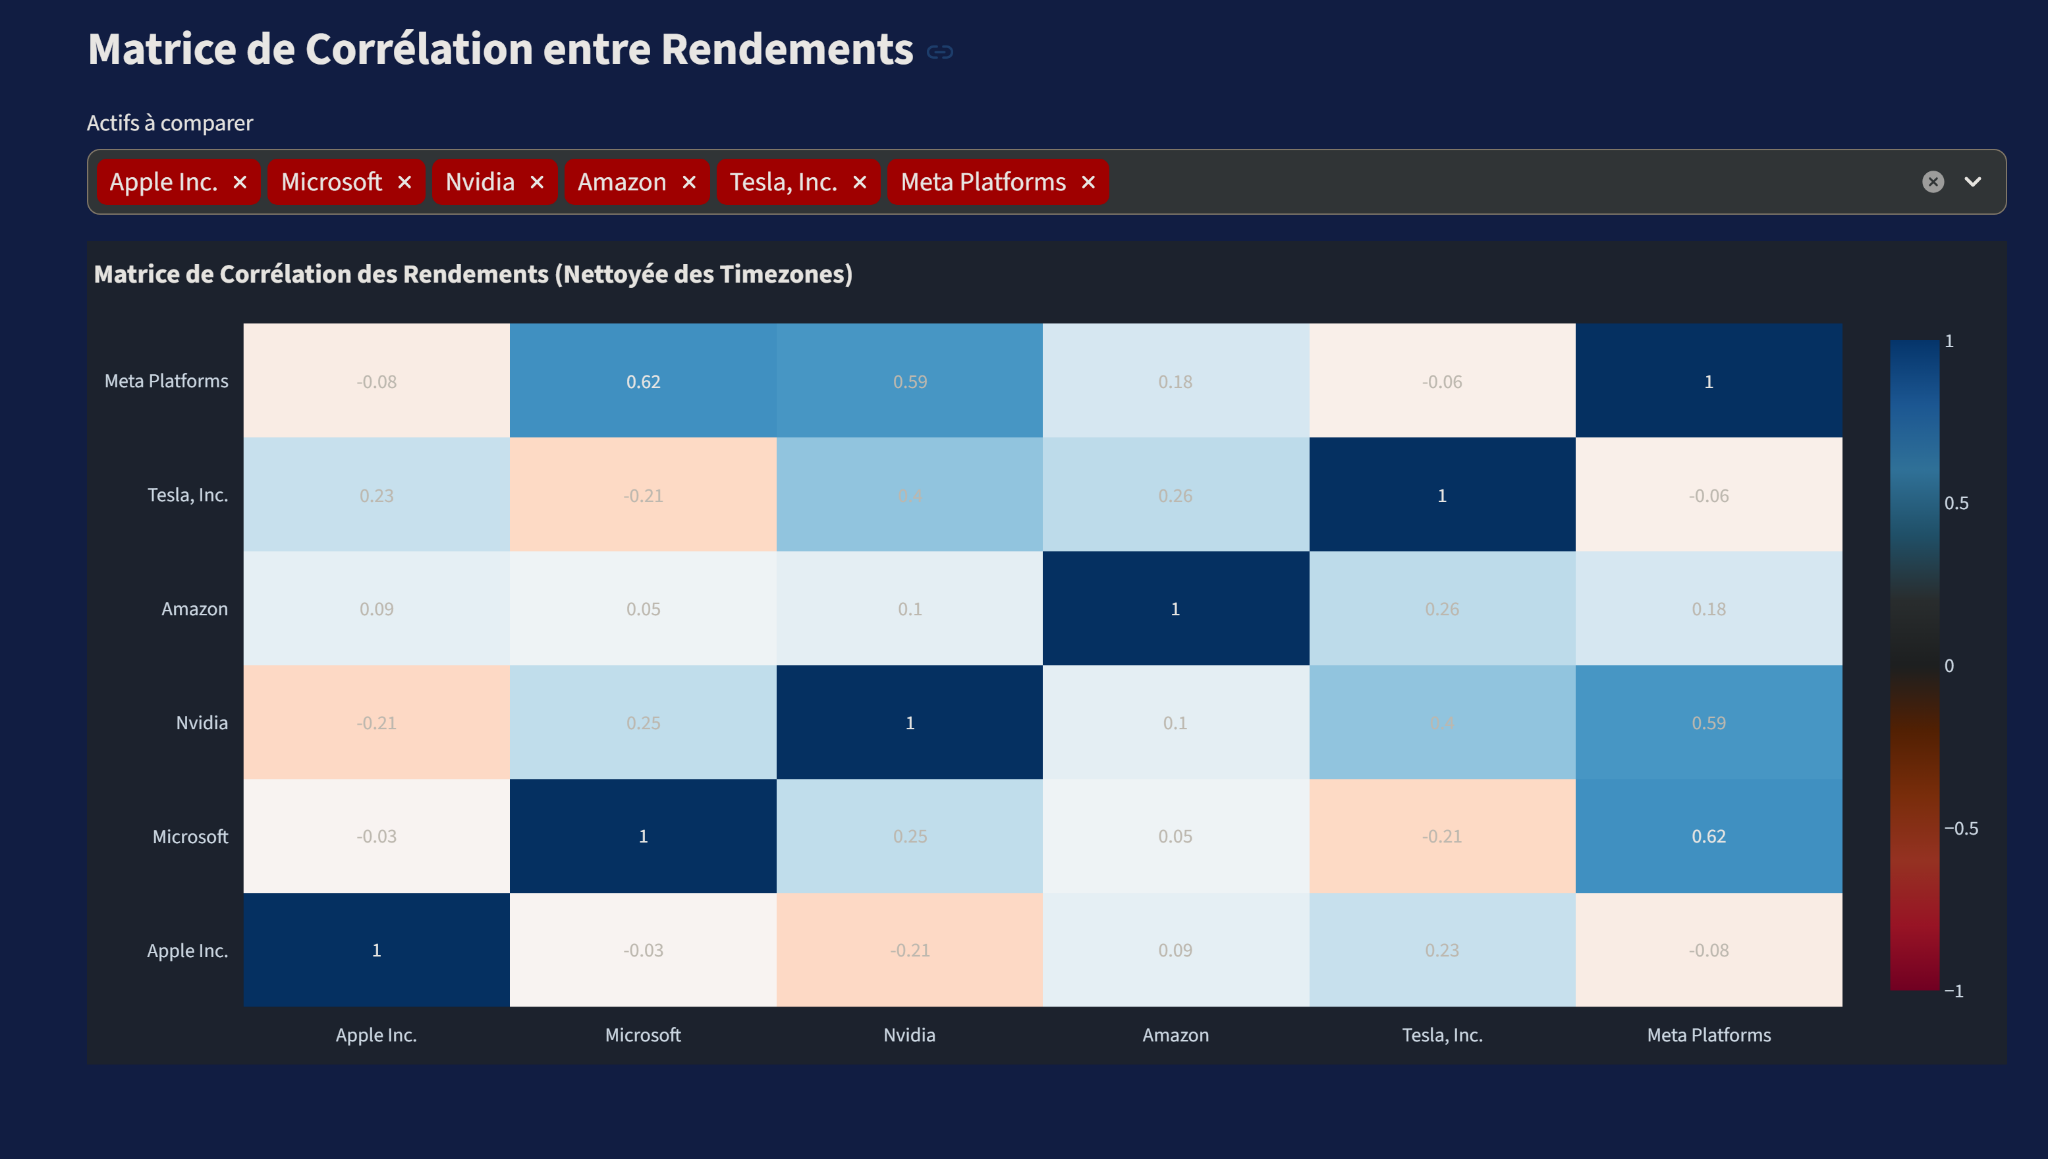
\includegraphics[width=\linewidth]{./media/image5.png}
 
    \textbf{Page 3 --- Portefeuille (passer un ordre)}
 
    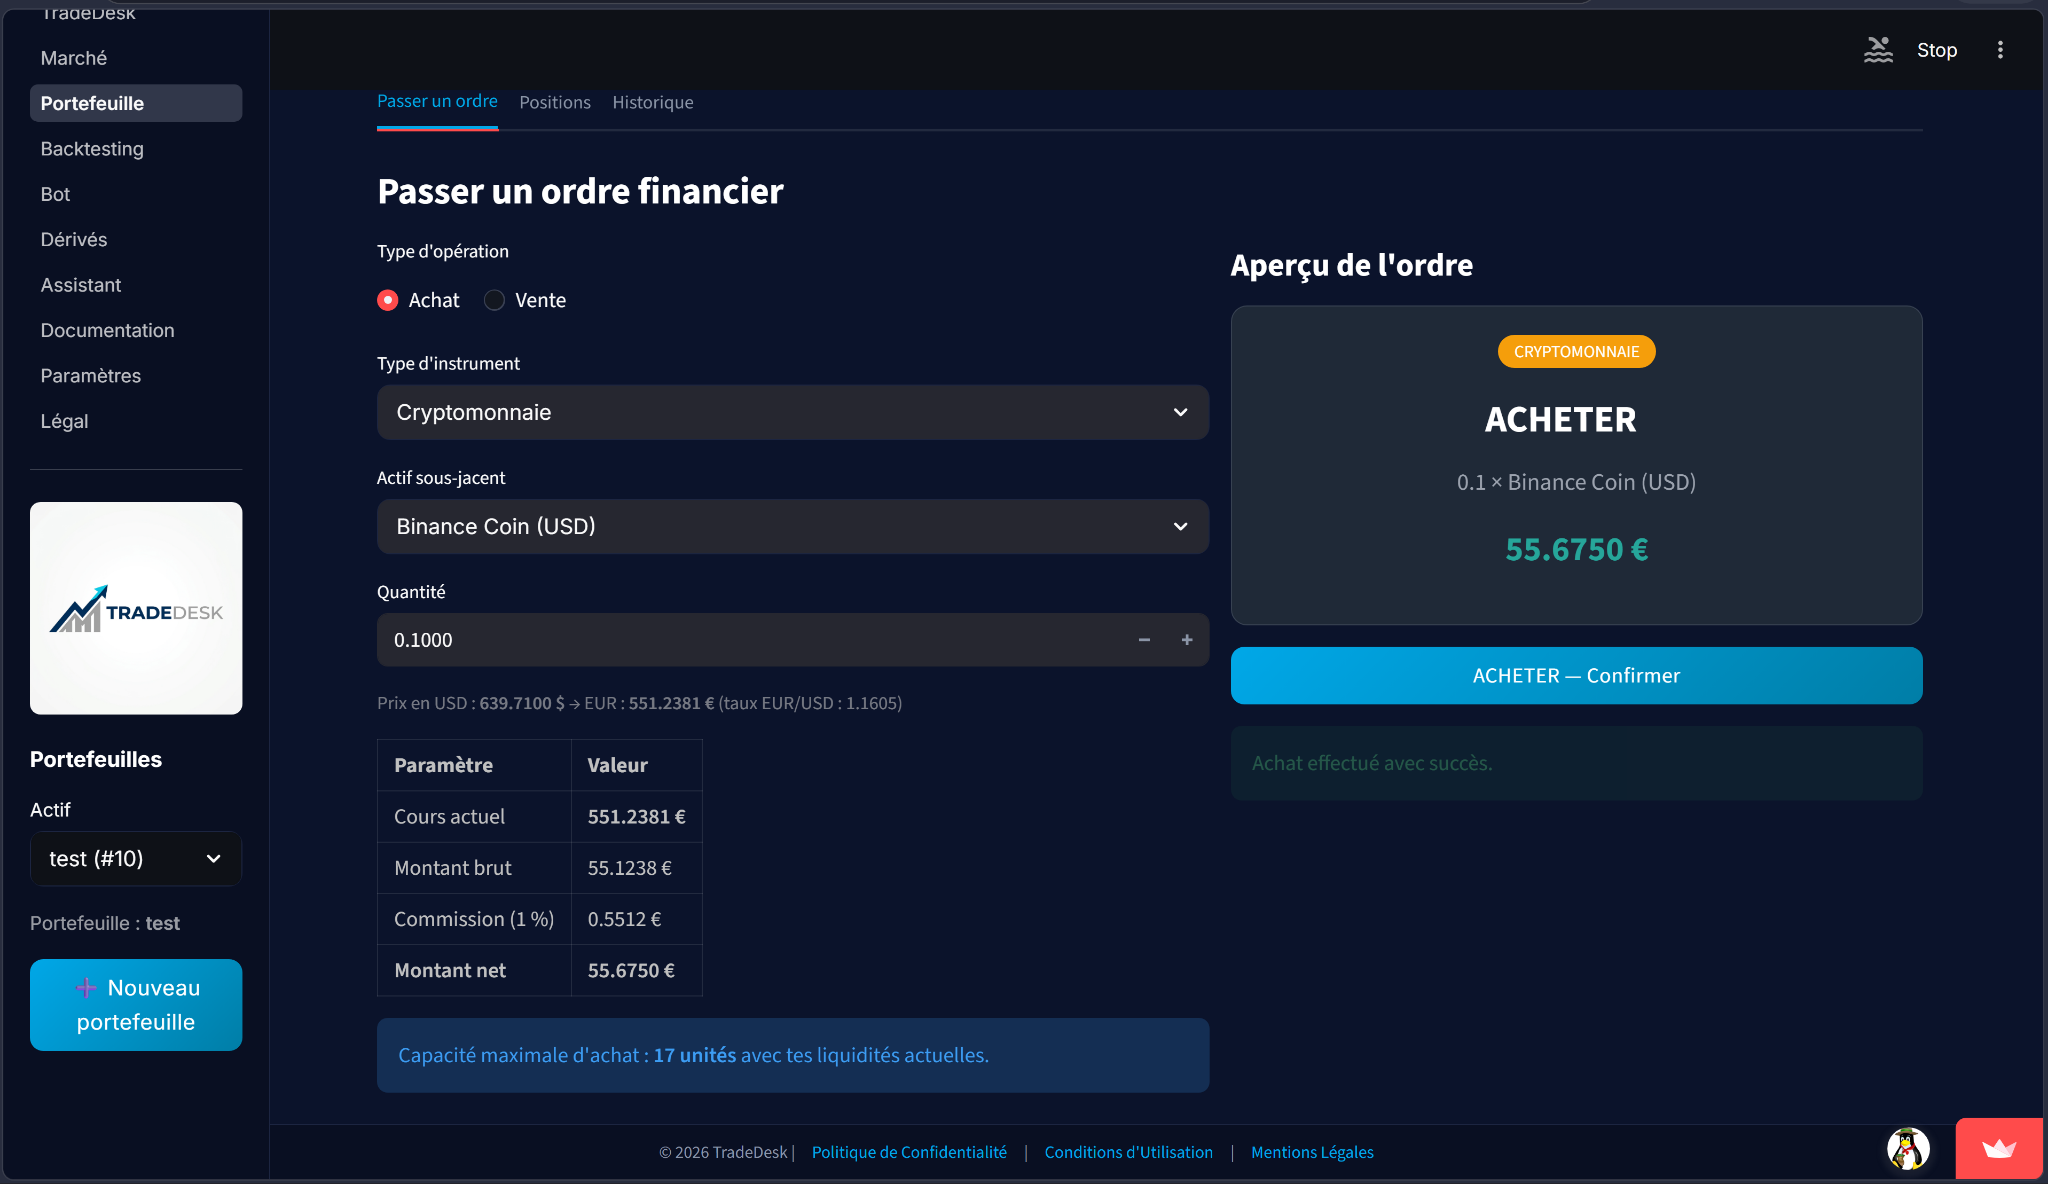
\includegraphics[width=\linewidth]{./media/image23.png}
 
    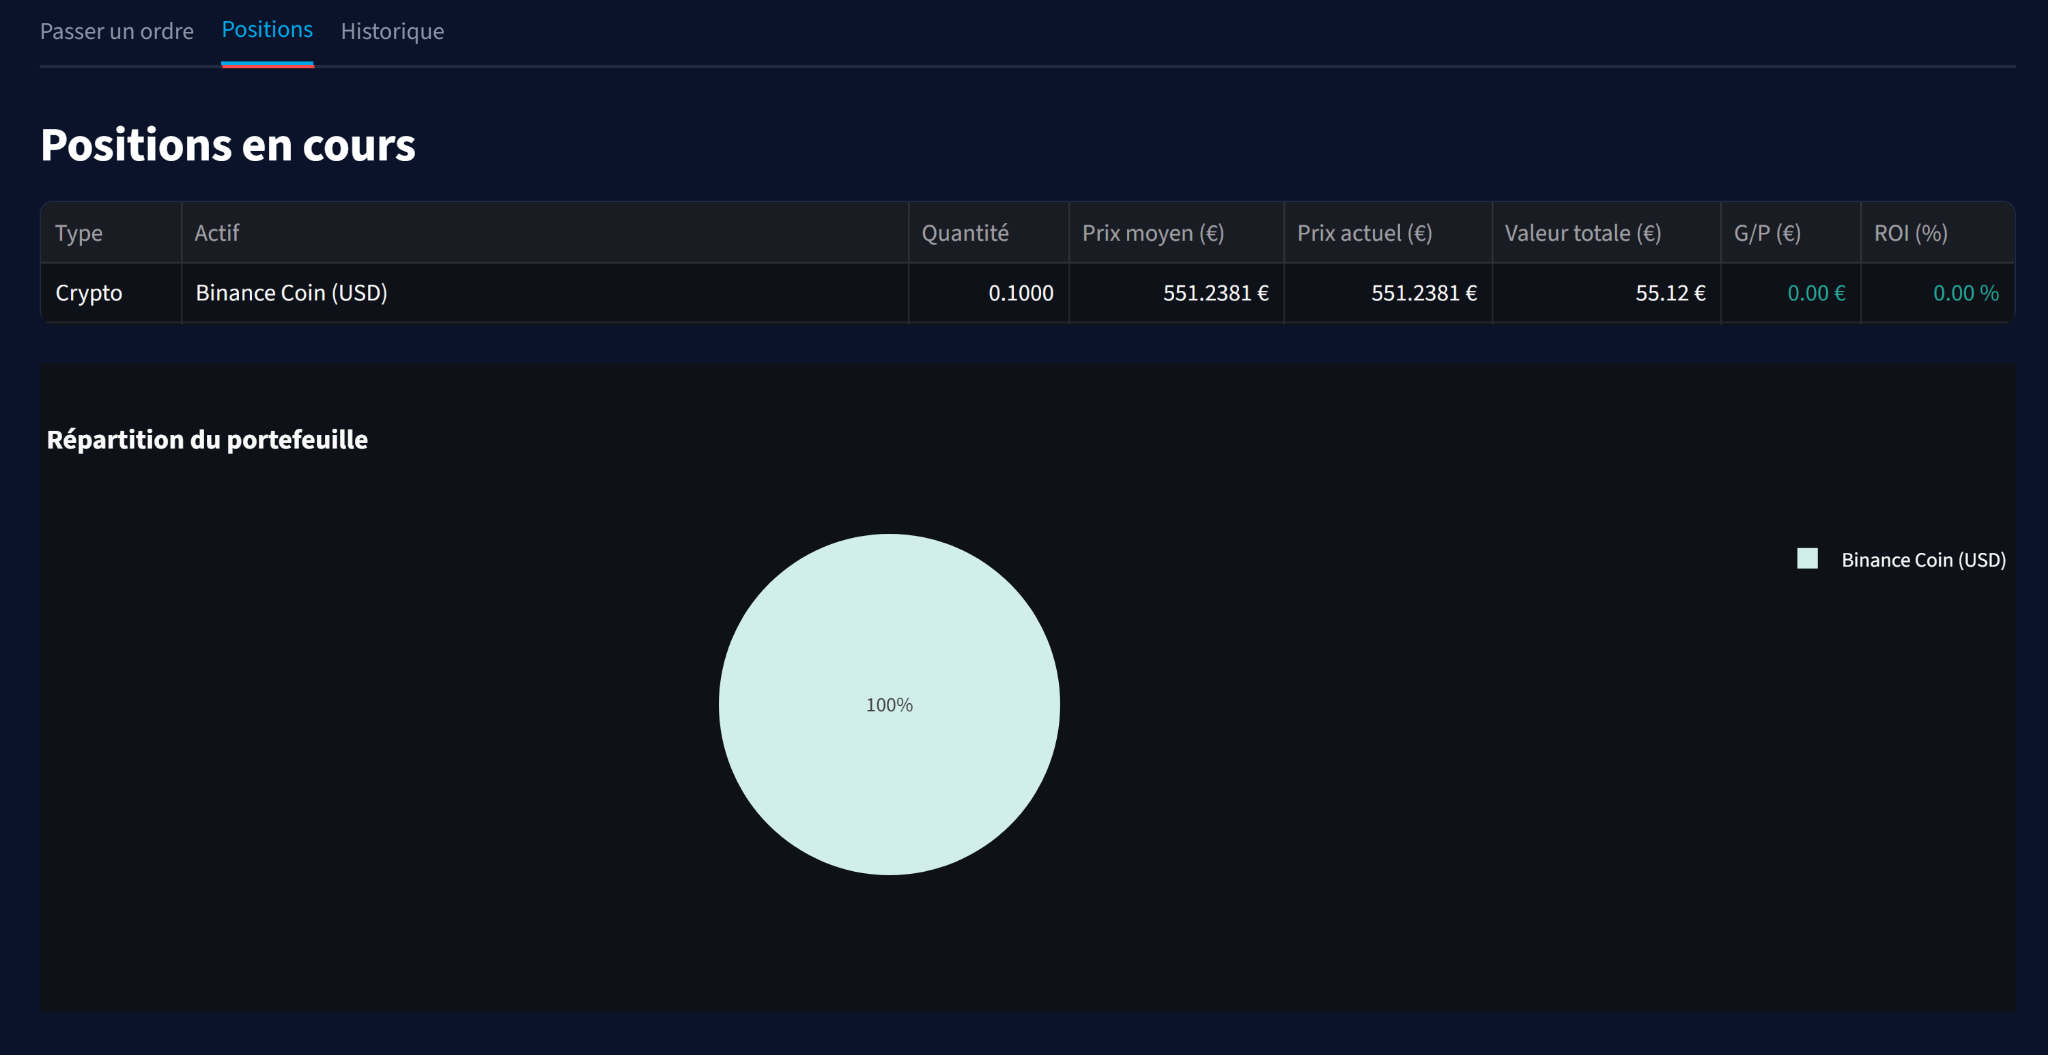
\includegraphics[width=\linewidth]{./media/image11.png}
 
    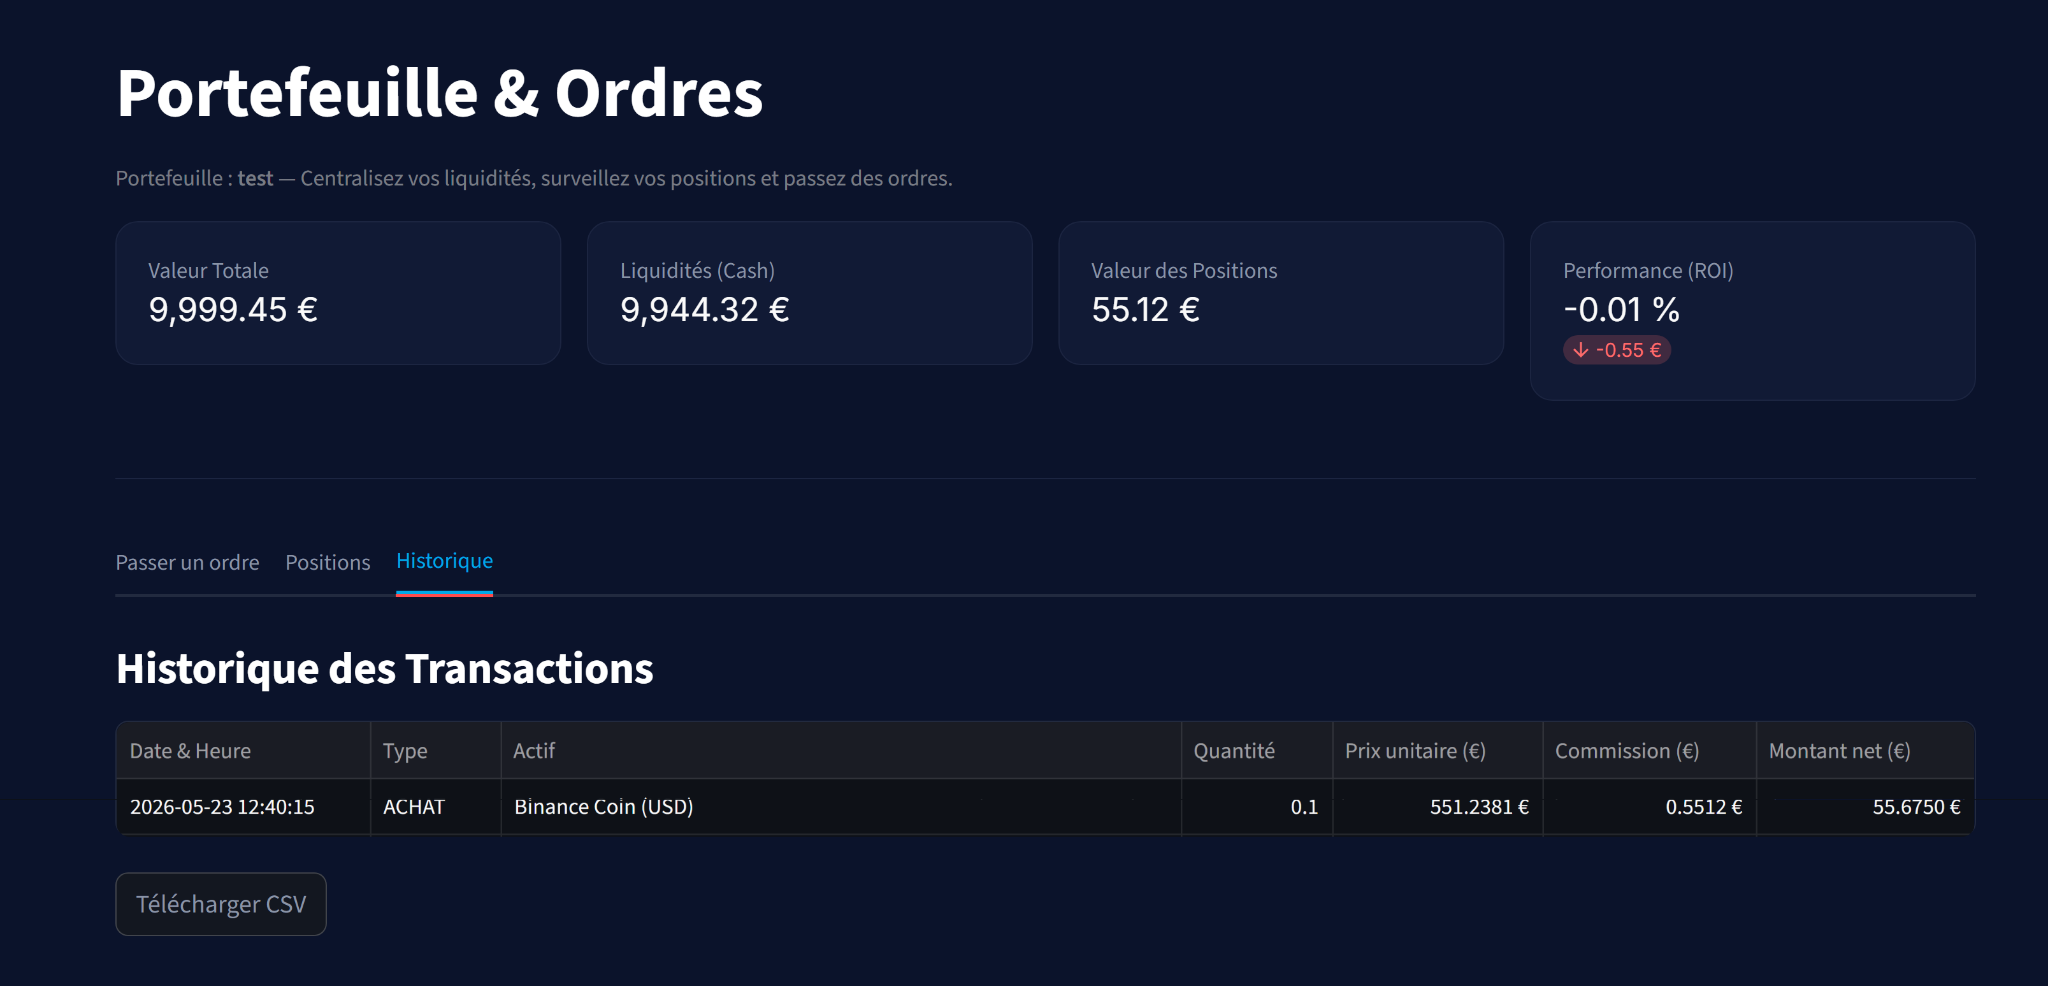
\includegraphics[width=\linewidth]{./media/image4.png}
 
    \textbf{Page 4 --- Backtesting (résultats d'une stratégie SMA)}
 
    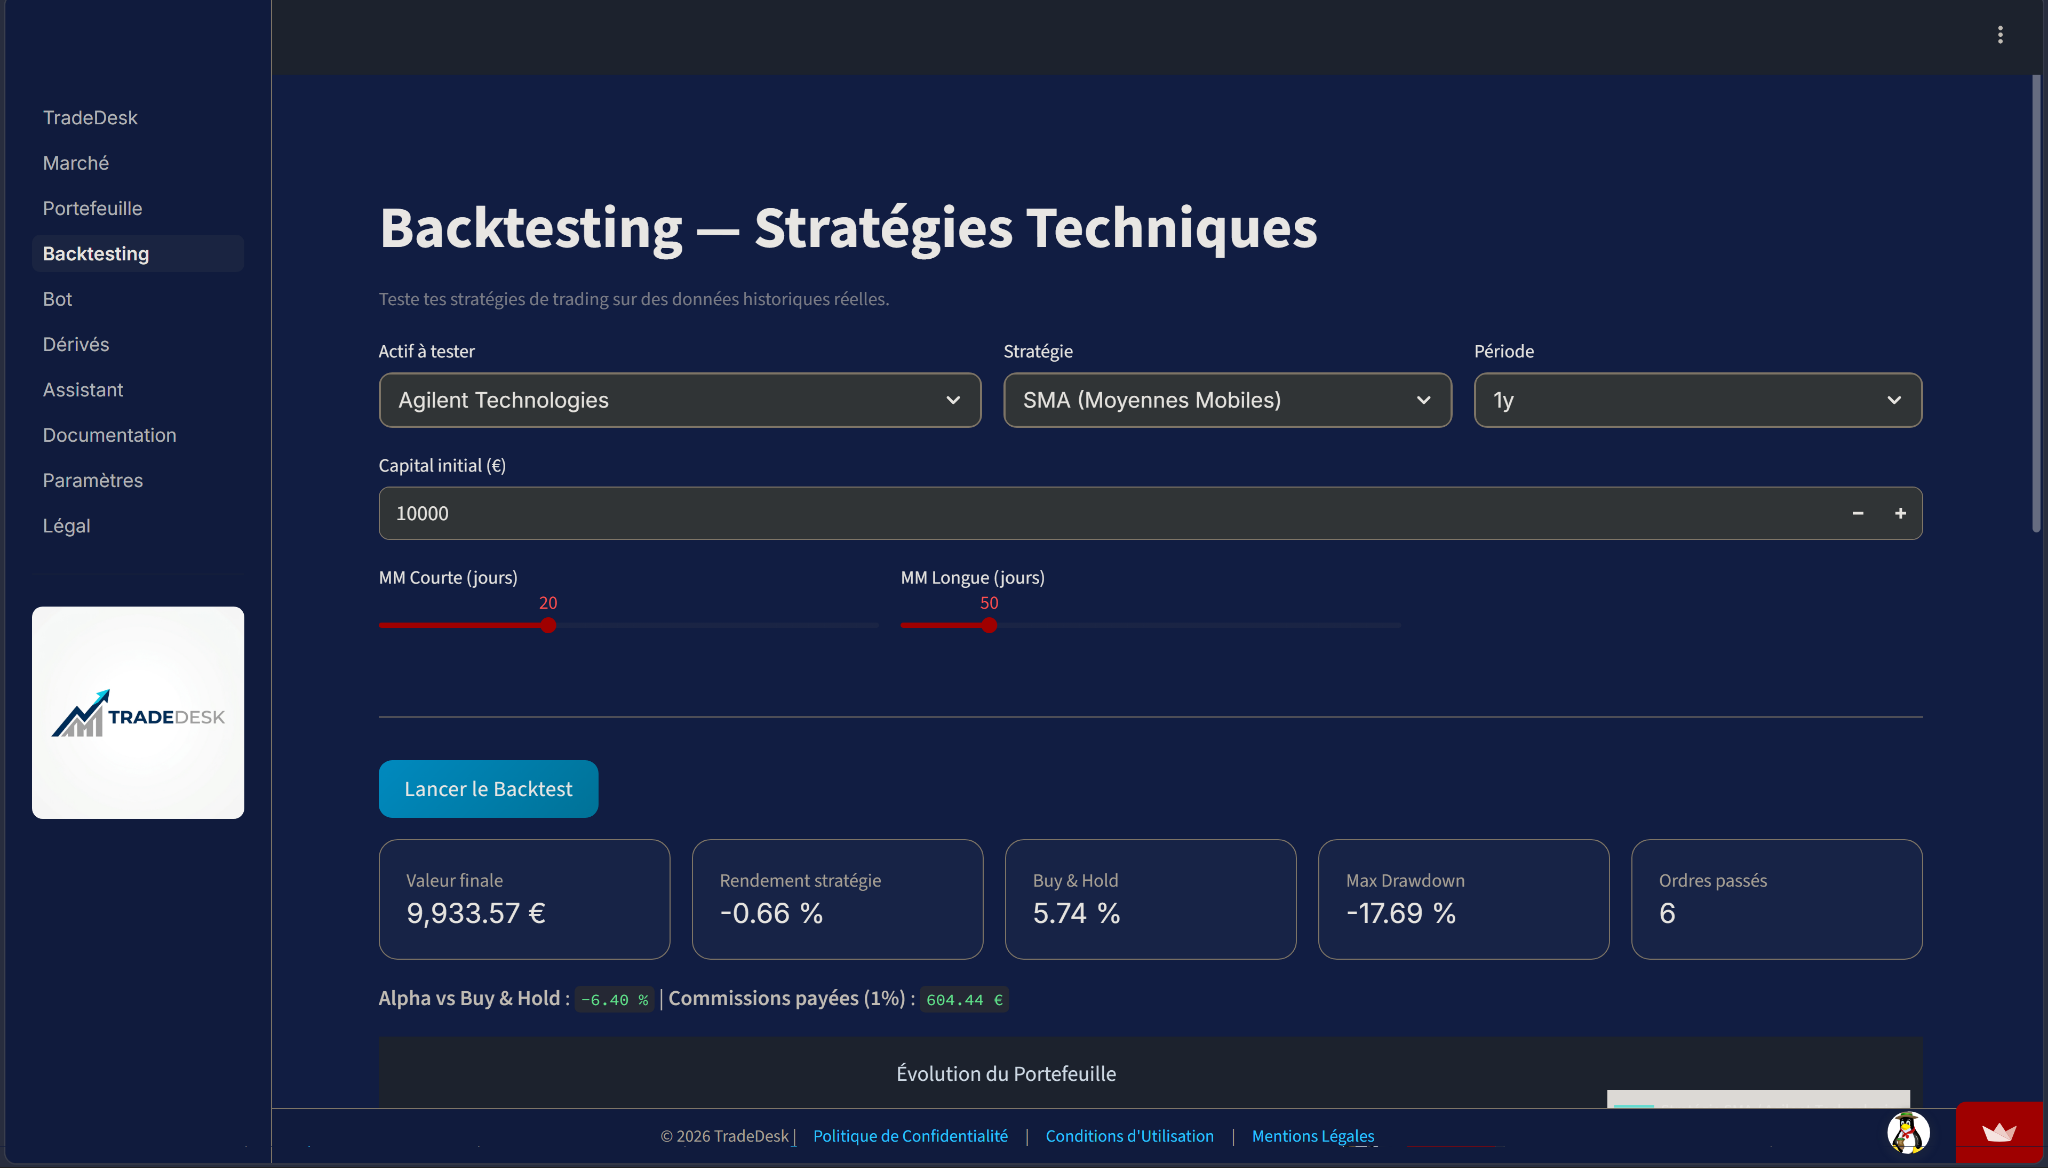
\includegraphics[width=\linewidth]{./media/image16.png}
 
    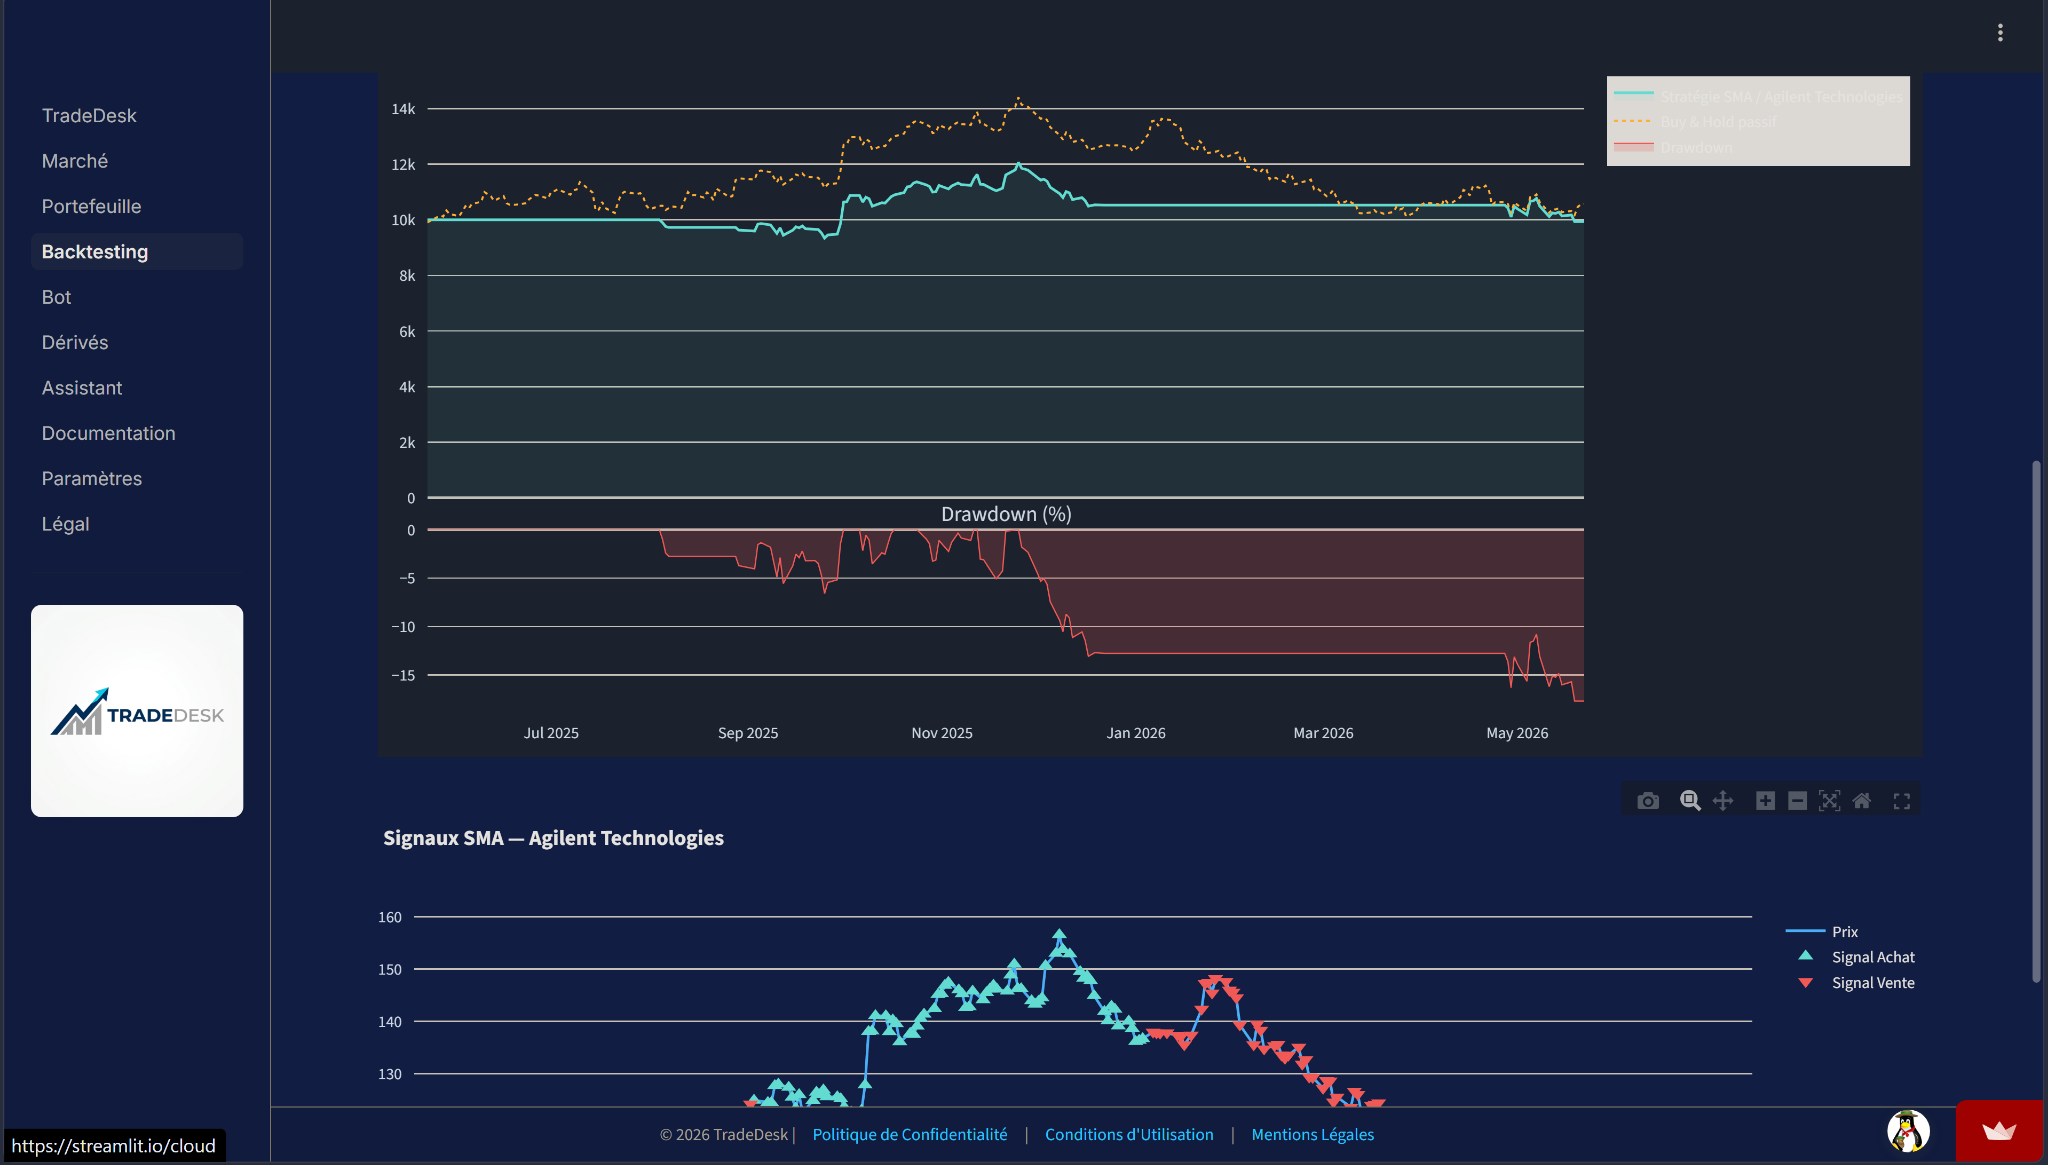
\includegraphics[width=\linewidth]{./media/image27.png}
 
    \textbf{Page 5 --- Bot de trading (rapport d'analyse ML)}
 
    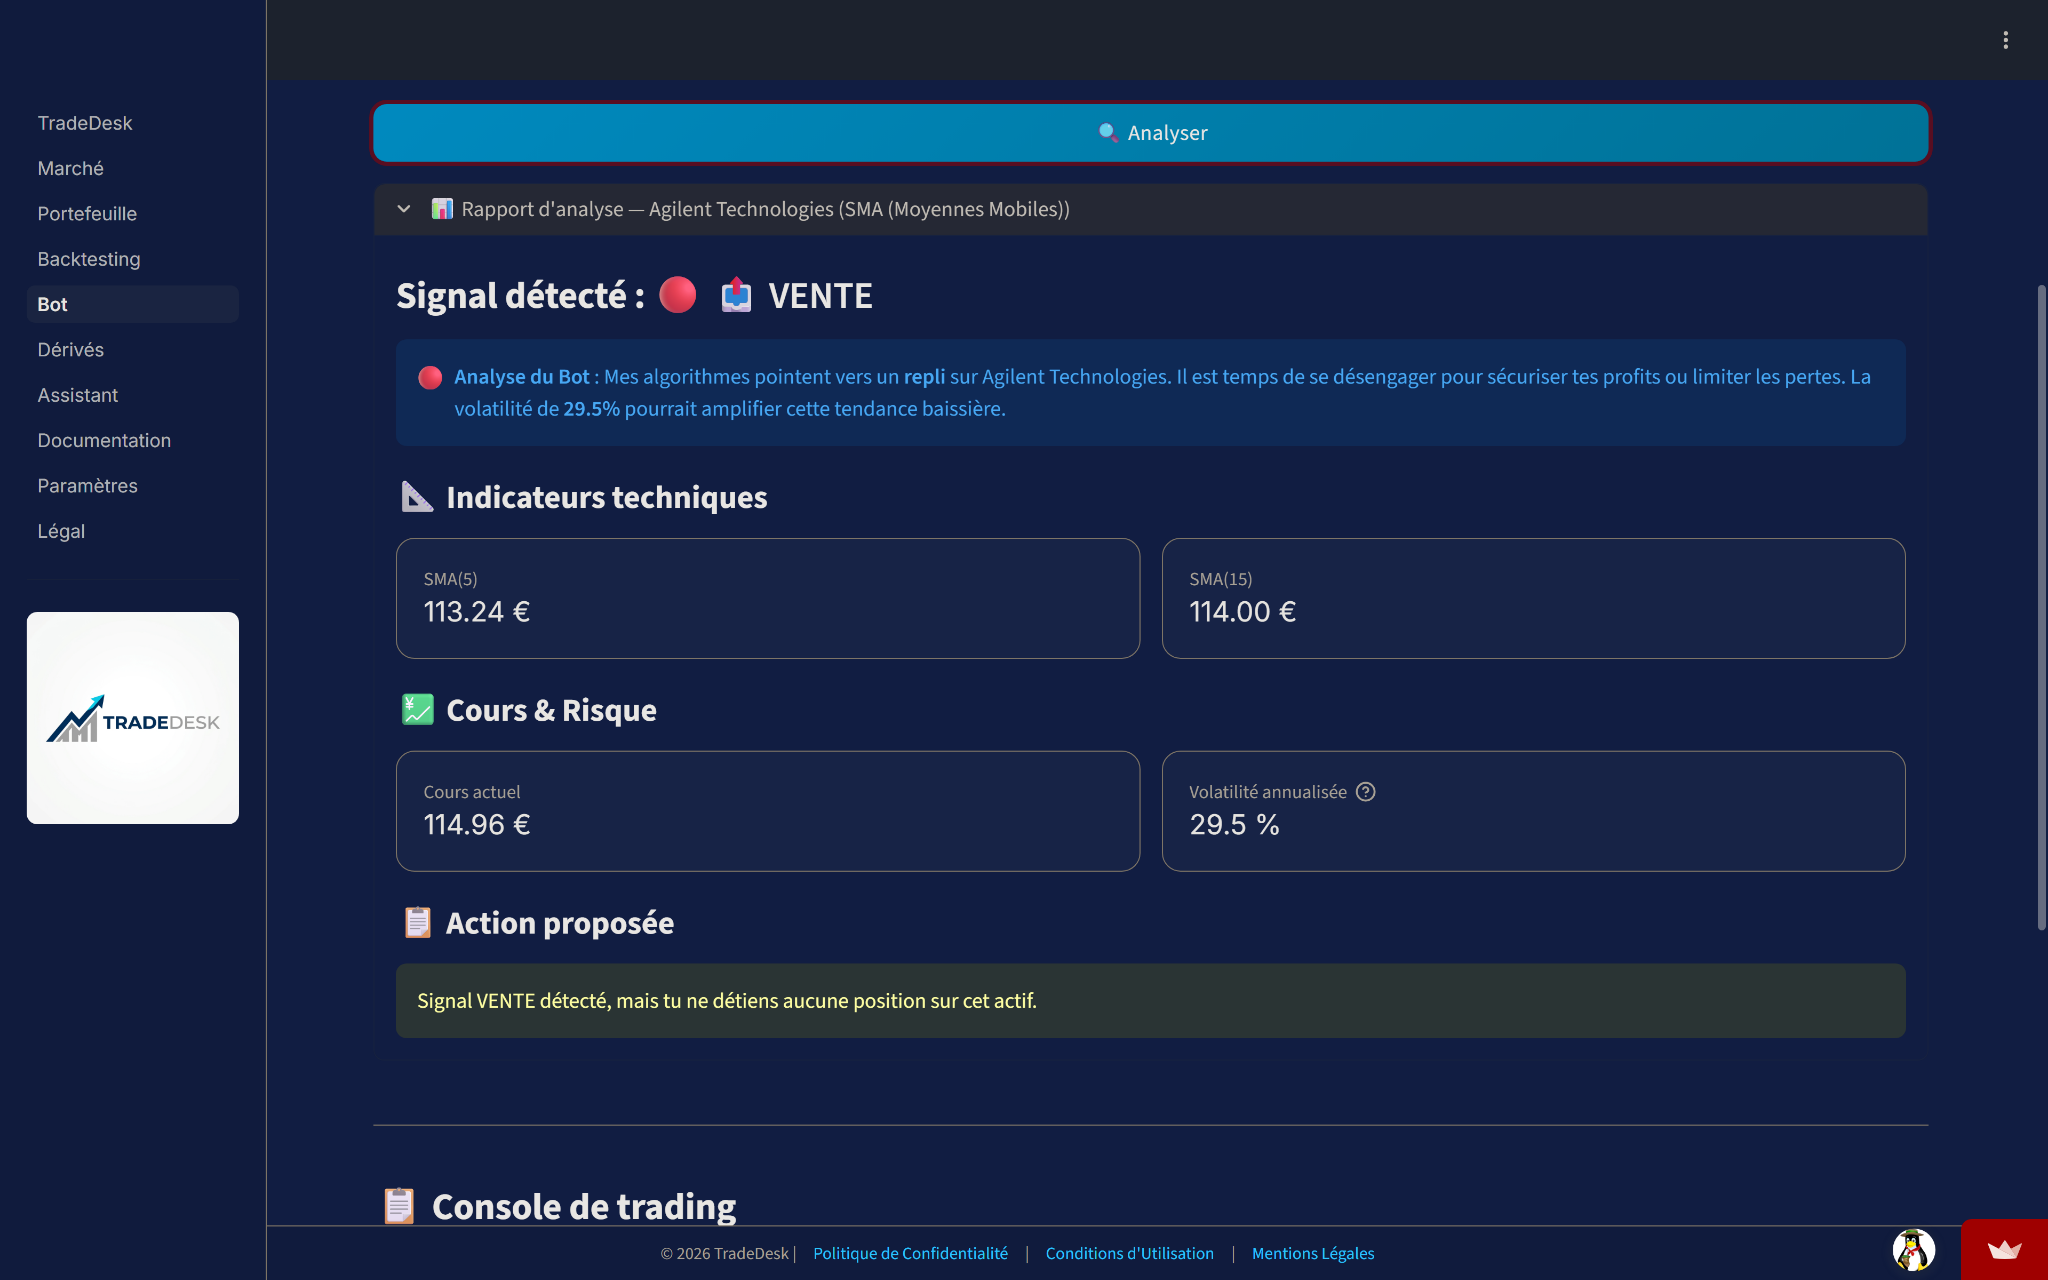
\includegraphics[width=\linewidth]{./media/image2.png}
 
    \textbf{Page 6 --- Dérivés (surface 3D Black-Scholes)}
 
    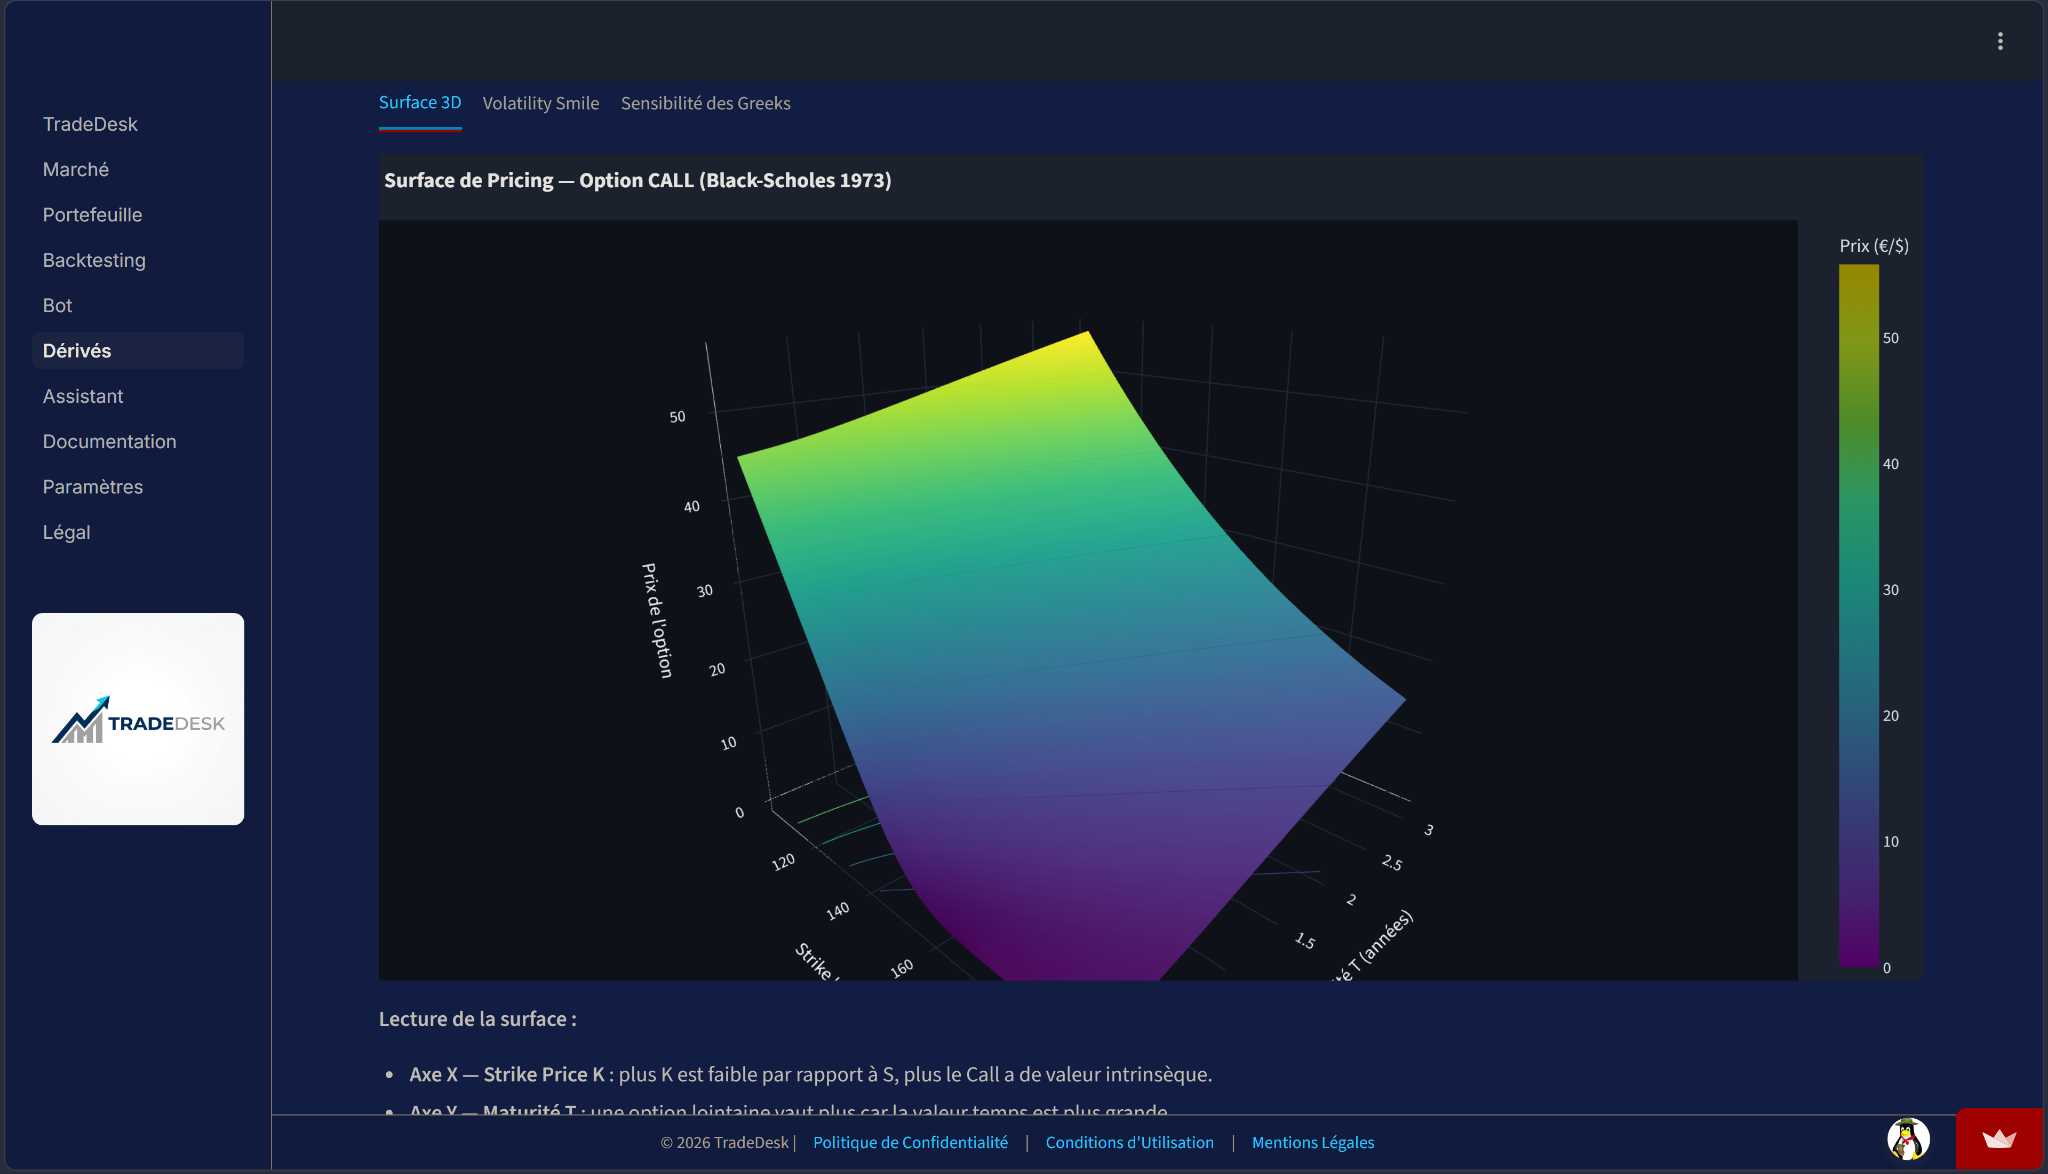
\includegraphics[width=\linewidth]{./media/image20.png}
 
    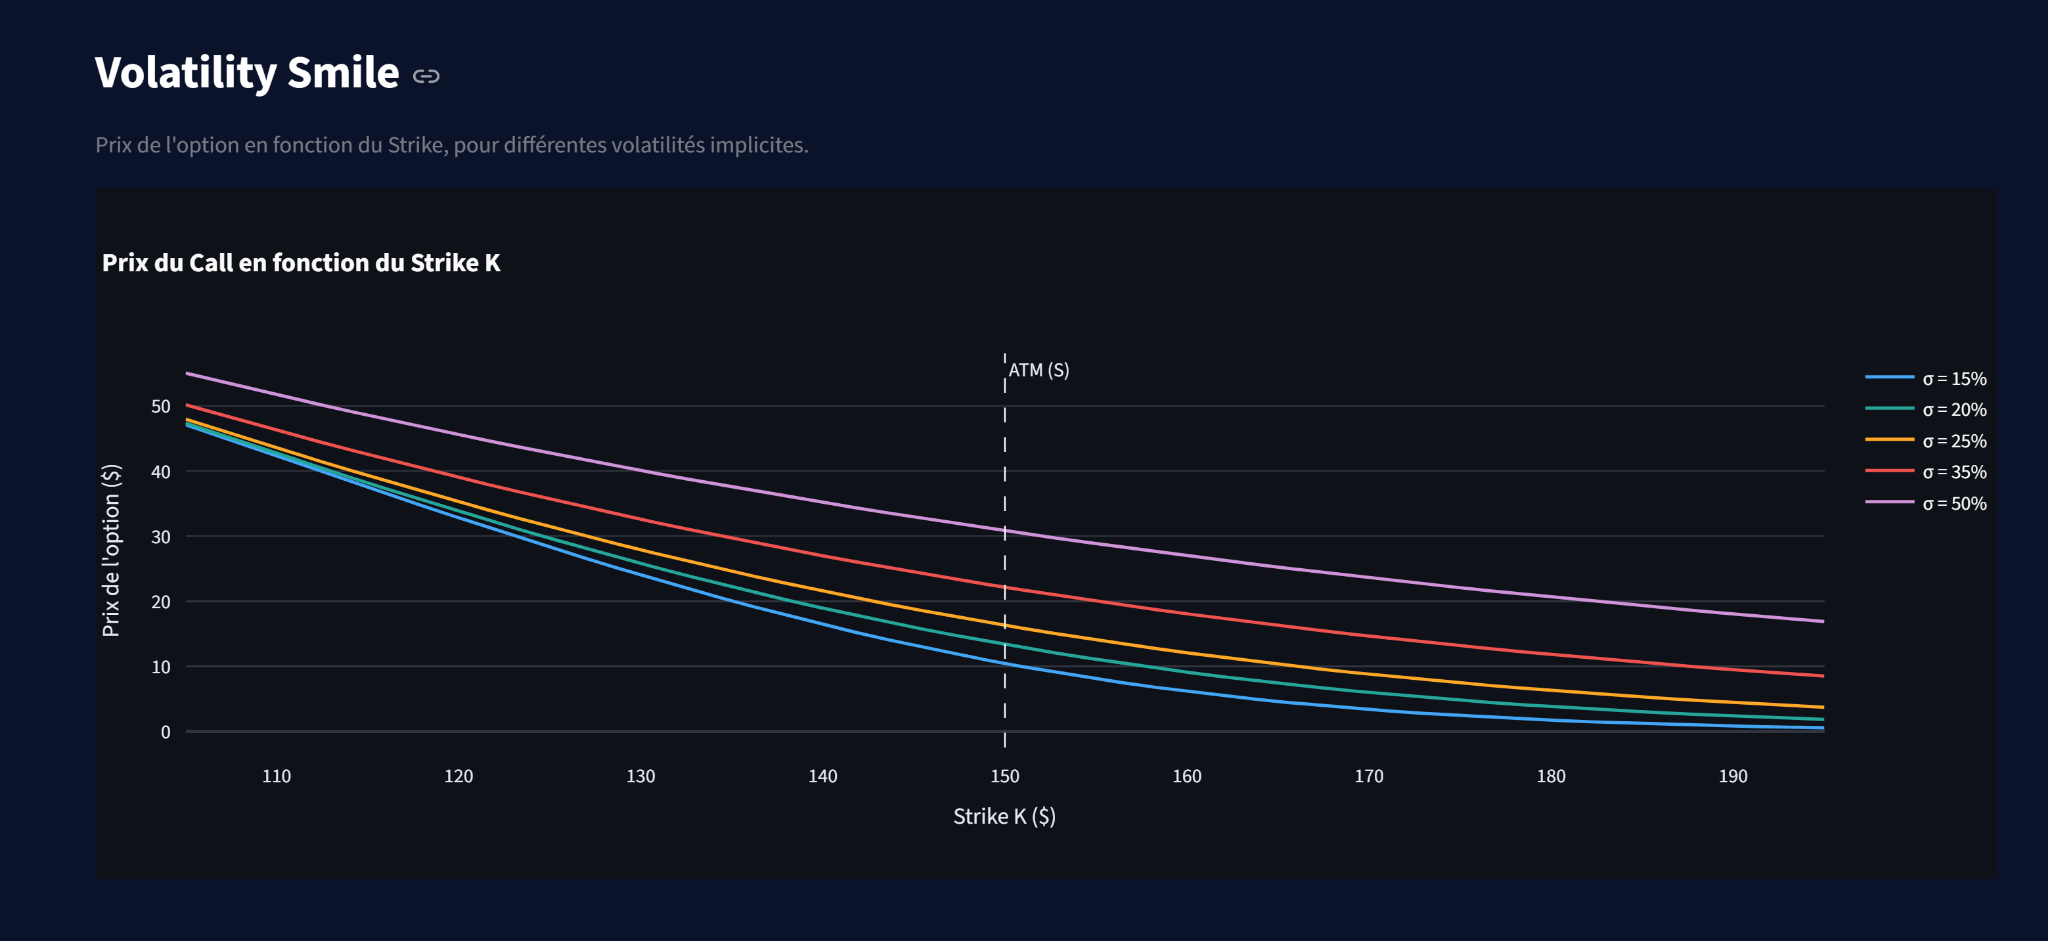
\includegraphics[width=\linewidth]{./media/image15.png}
 
    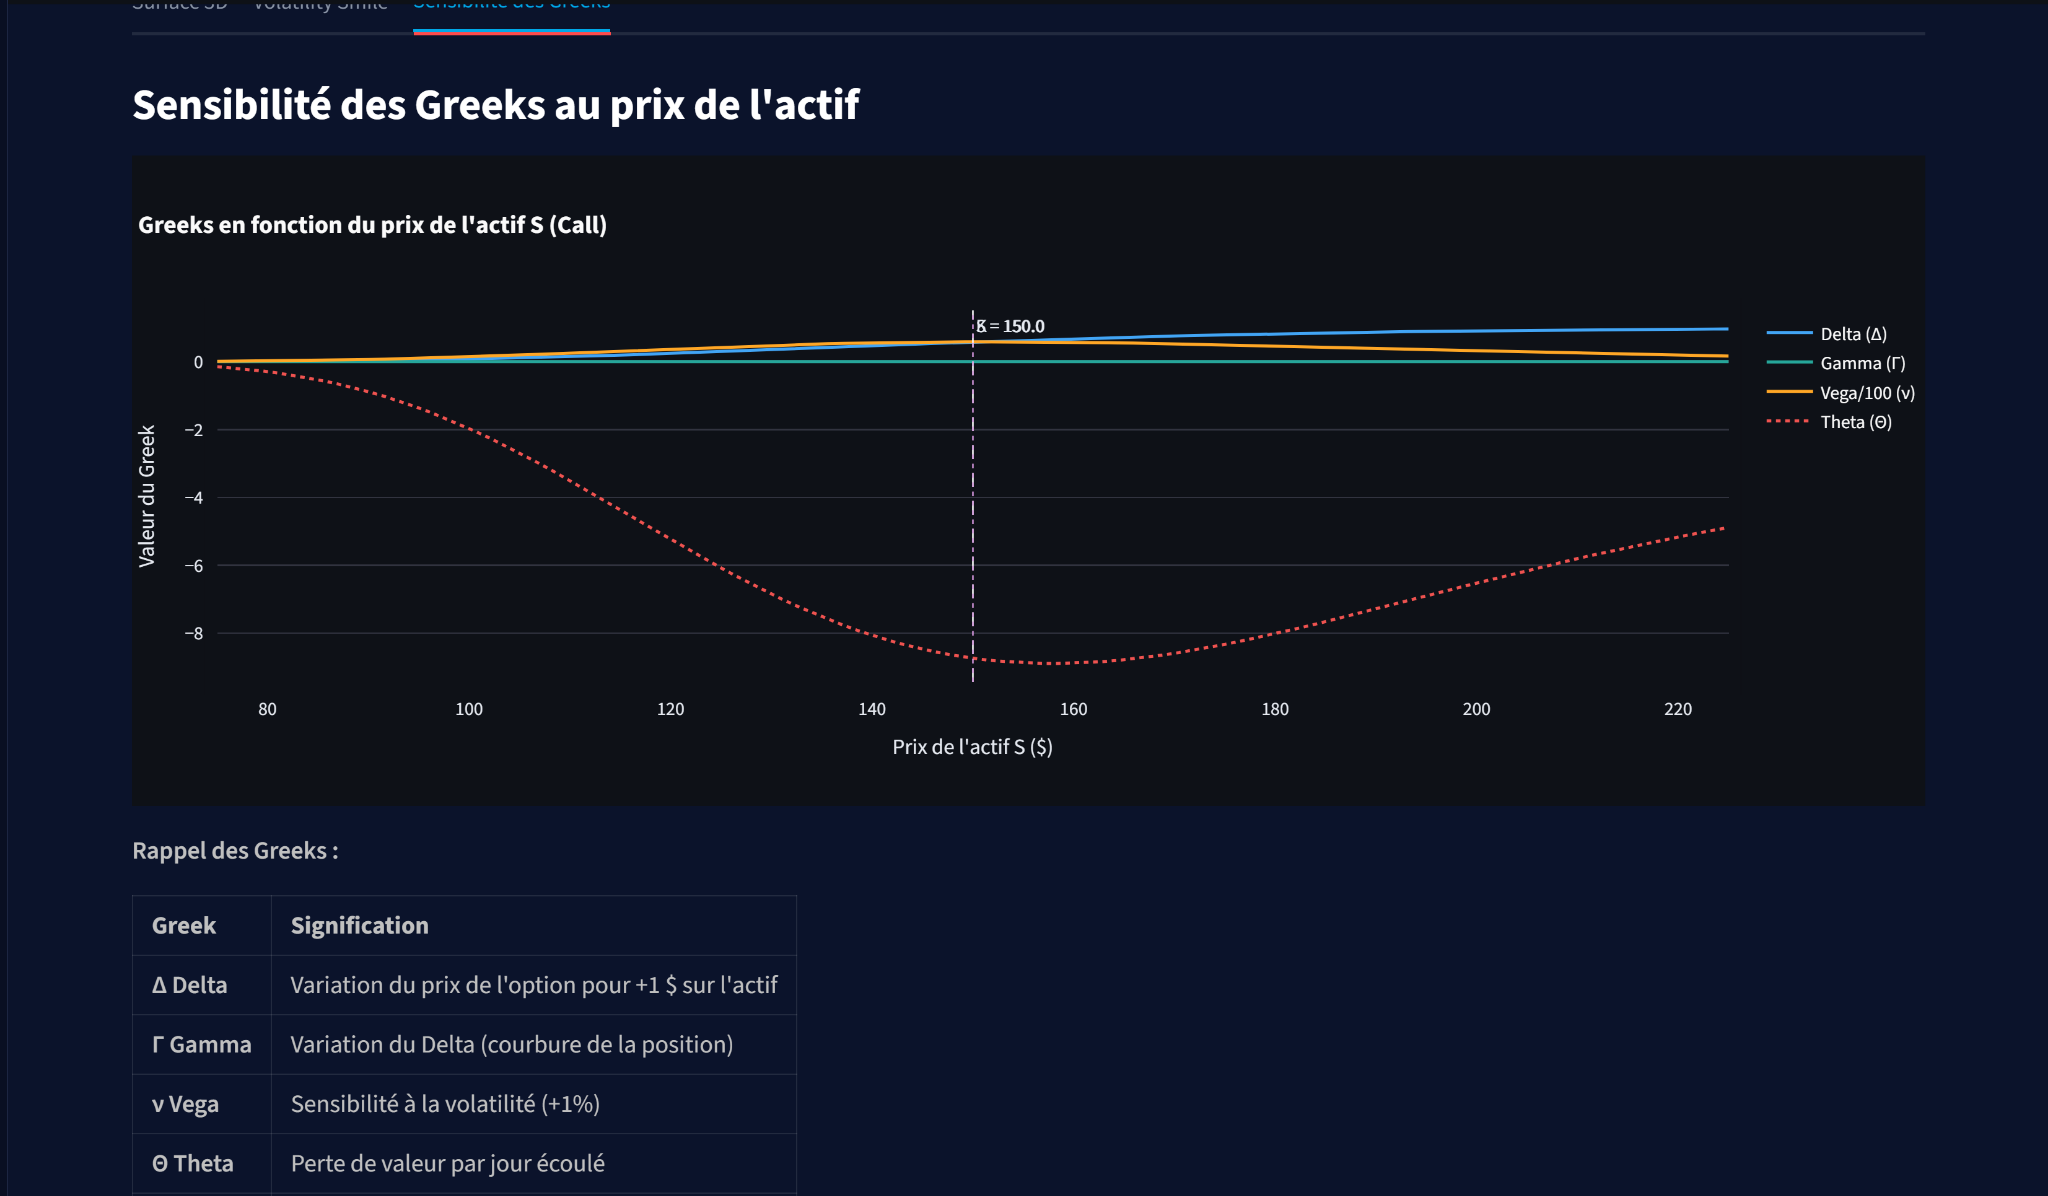
\includegraphics[width=\linewidth]{./media/image6.png}
 
    \textbf{Page 7 --- Assistant}
 
    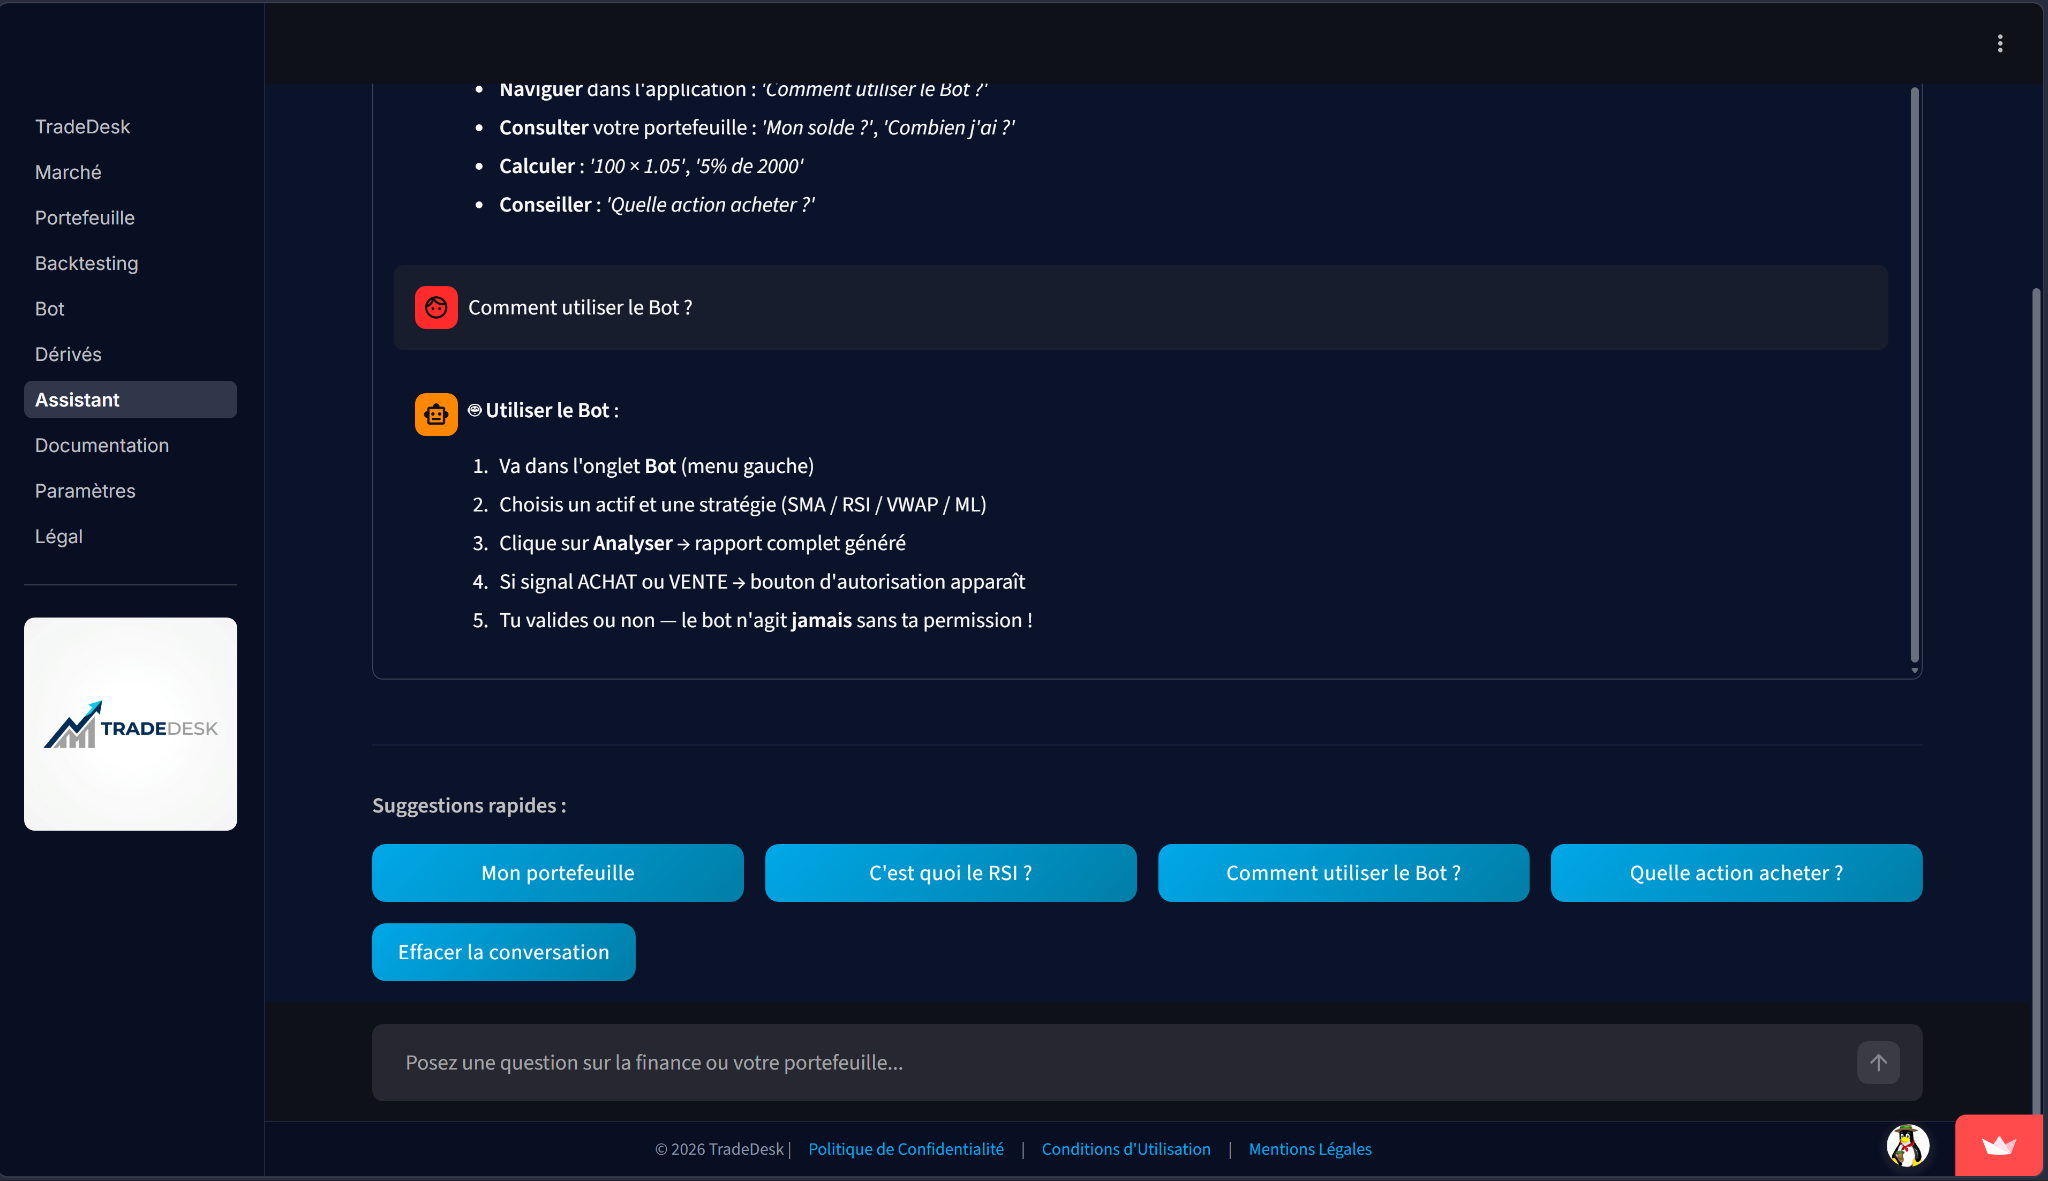
\includegraphics[width=\linewidth]{./media/image13.png}
 
    \textbf{Page 8 --- Documentation}
 
    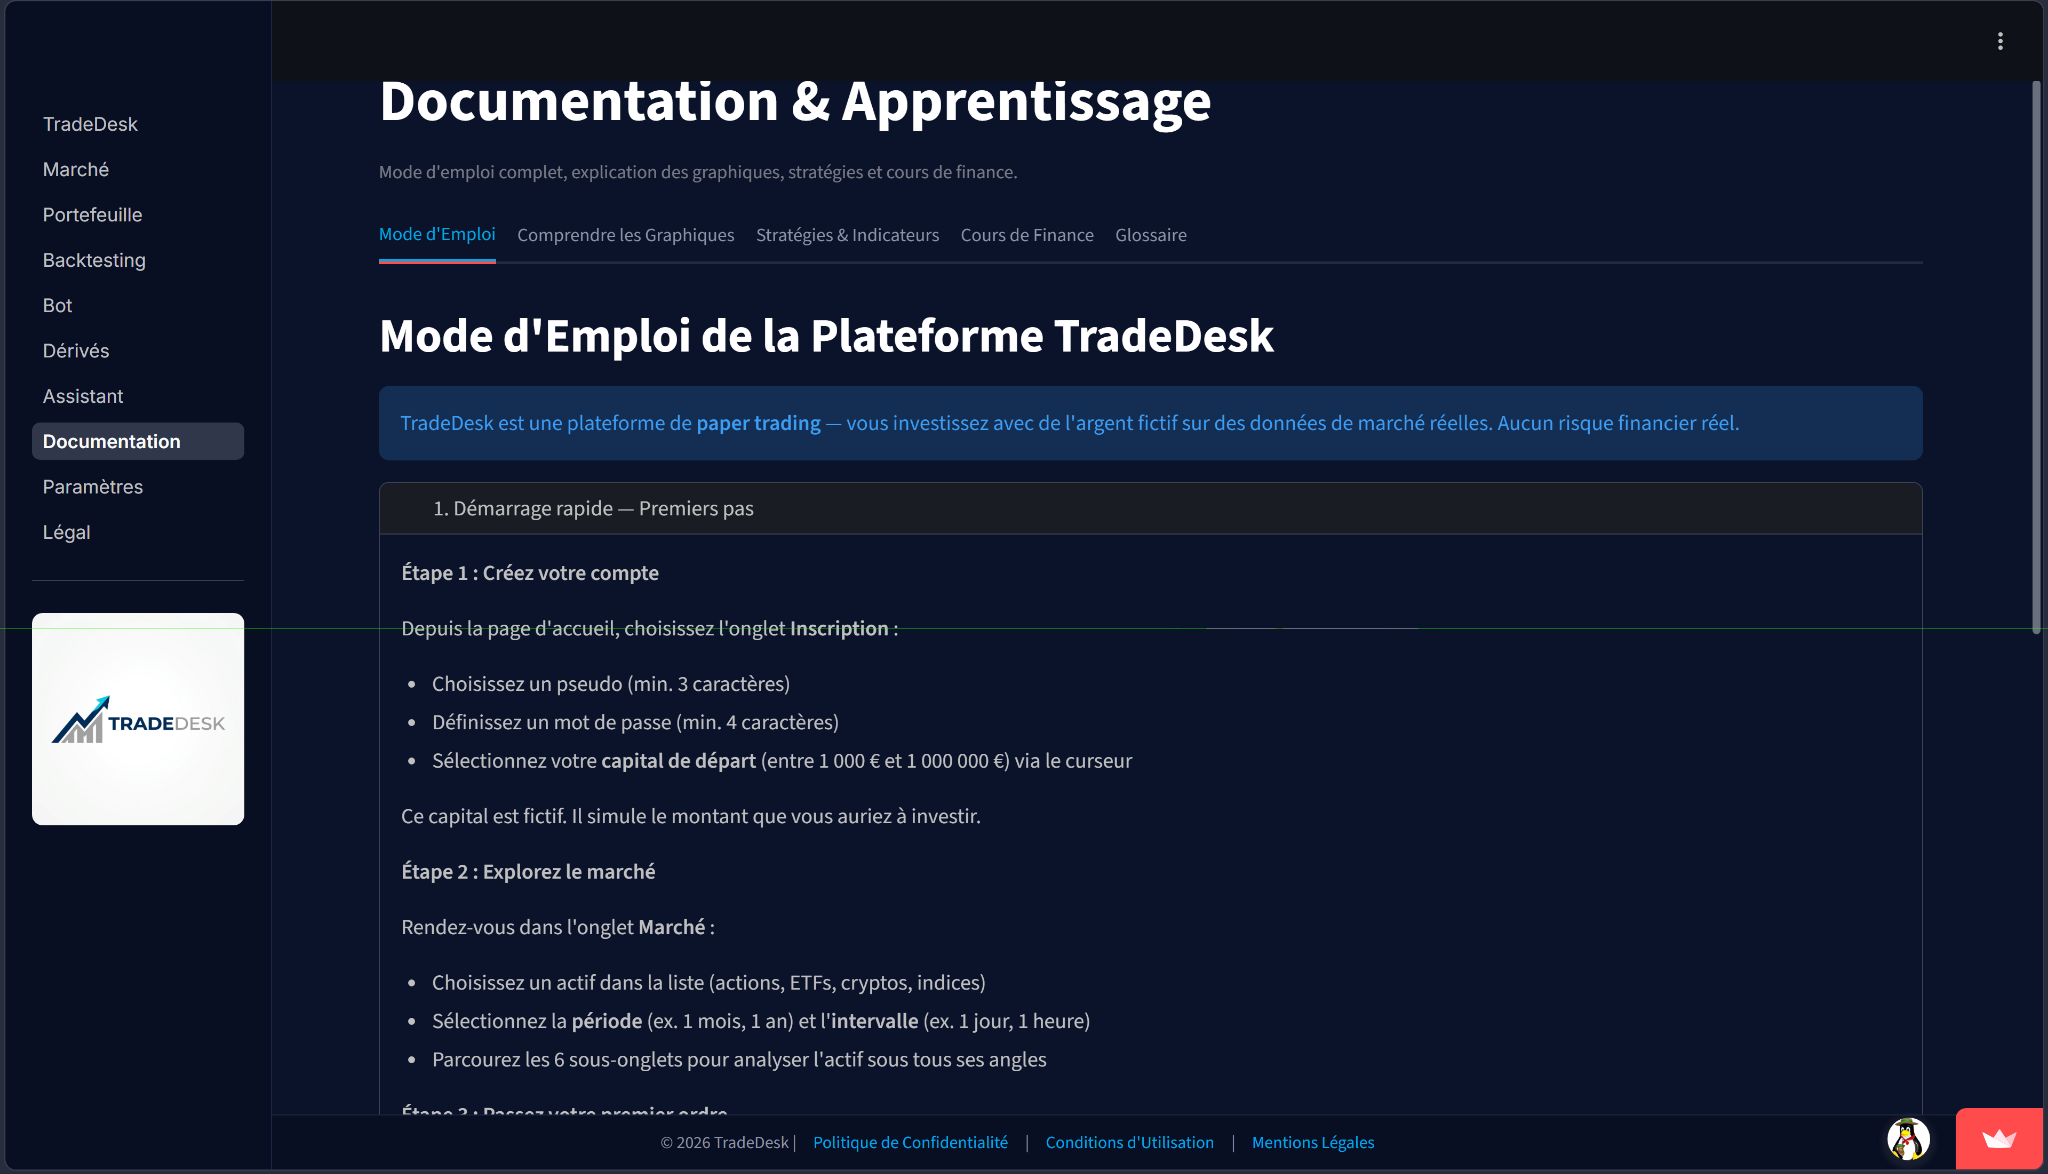
\includegraphics[width=\linewidth]{./media/image3.png}
 
    \textbf{Page 9 --- Paramètres}
 
    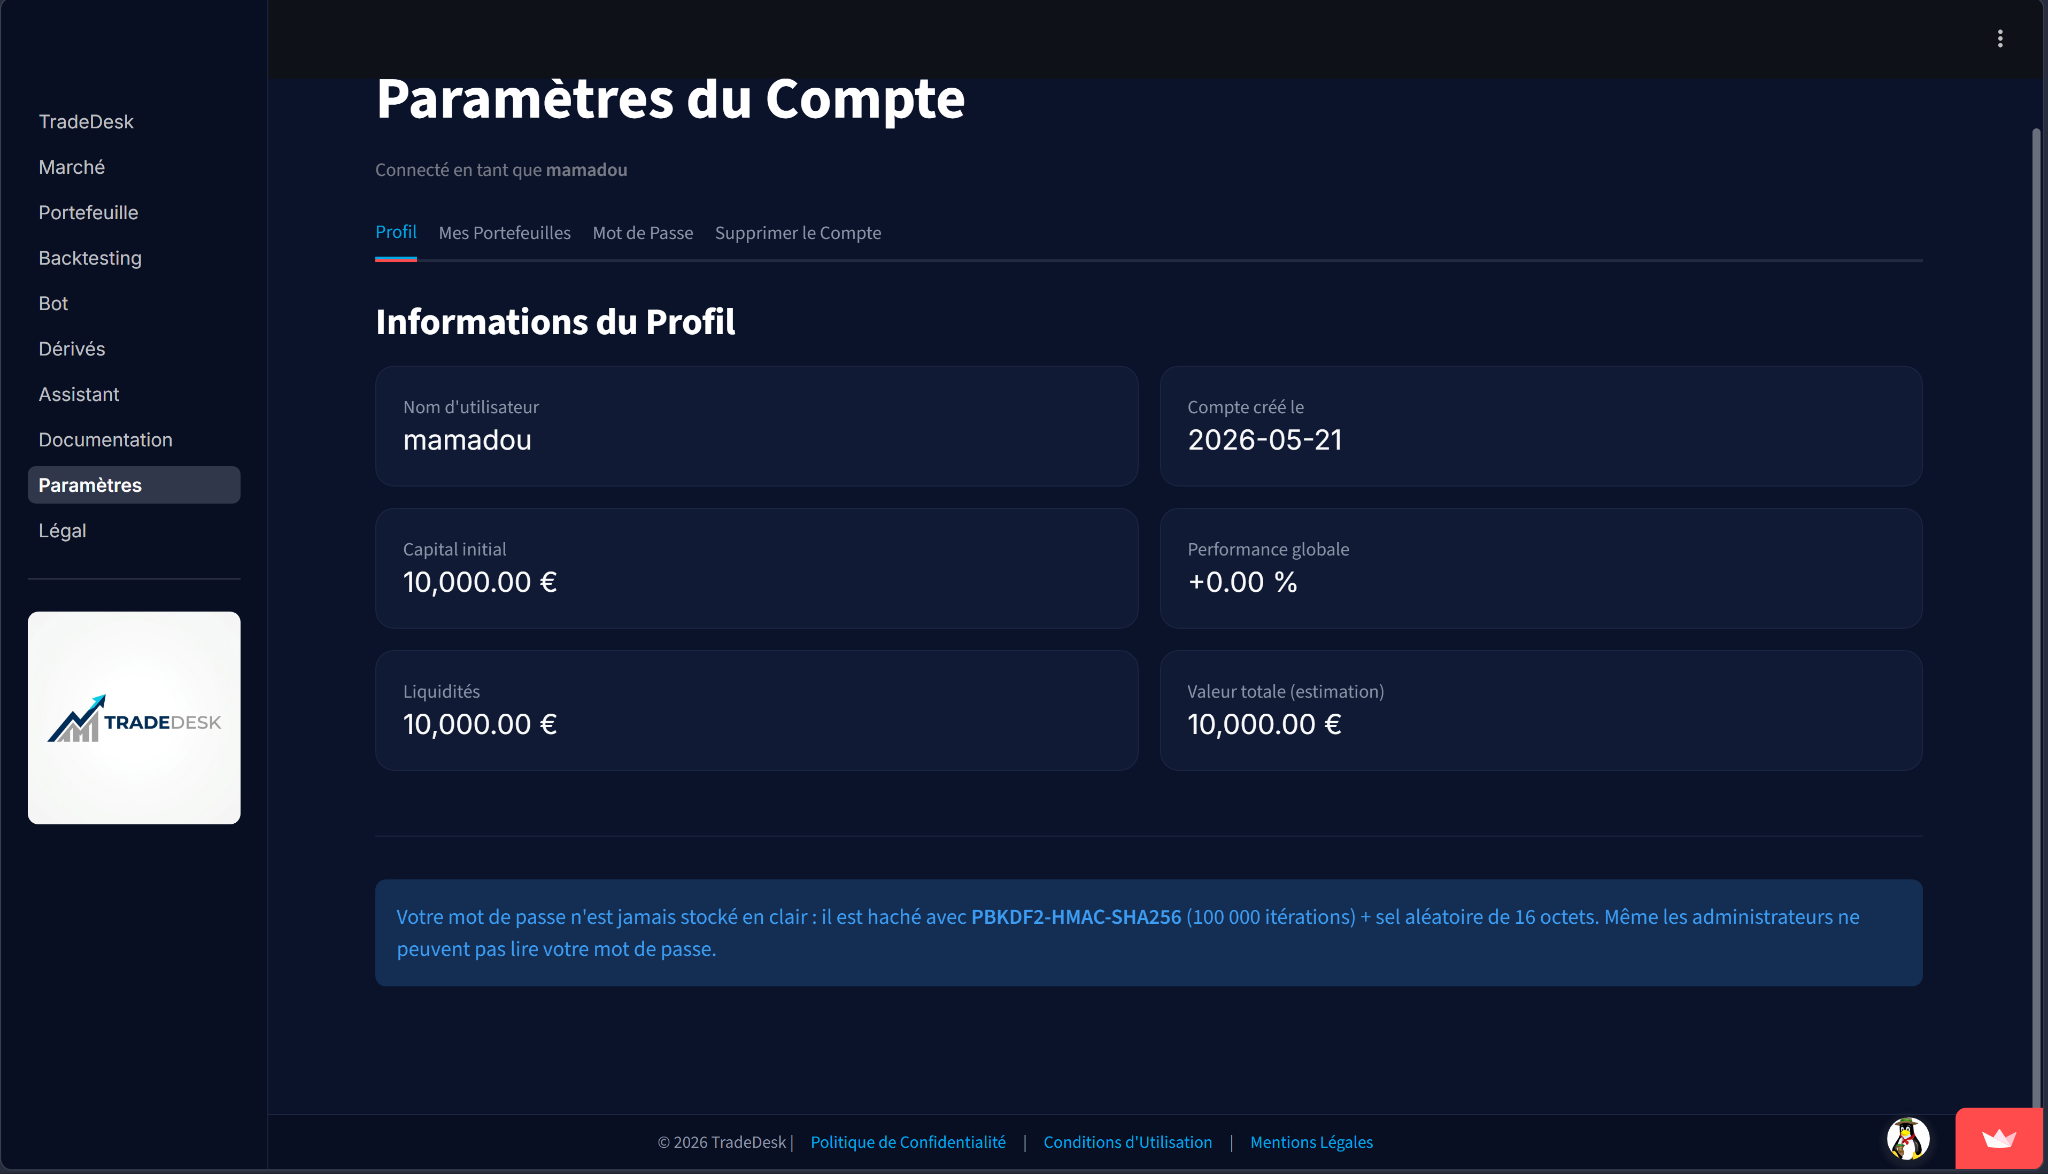
\includegraphics[width=\linewidth]{./media/image8.png}

    \section{Manuel utilisateur}

    \subsection*{Prérequis}

    Aucune installation n'est nécessaire côté utilisateur. Il suffit d'un
    navigateur web (Chrome, Firefox, Safari) et d'une connexion internet.
    L'application est accessible à l'adresse :
    \url{https://tradedesk-mety.streamlit.app/}

    \subsection*{Création d'un compte}
    \begin{enumerate}
        \item Sur la page d'accueil, cliquer sur l'onglet \textit{Inscription}.
        \item Saisir un nom d'utilisateur (minimum 3 caractères, unique).
        \item Saisir un mot de passe (minimum 4 caractères) et le confirmer.
        \item Régler le capital de départ avec le slider
              (entre 1~000 et 1~000~000 euros fictifs).
        \item Cliquer sur \textit{Créer mon compte}, puis se connecter via
              l'onglet \textit{Connexion}.
    \end{enumerate}

    \subsection*{Navigation}

    La barre latérale gauche donne accès à toutes les pages. Sur mobile, elle
    est accessible via le bouton hamburger en haut à gauche.

    \subsection*{Acheter un actif}
    \begin{enumerate}
        \item Aller dans \textit{Portefeuille} $\to$ onglet
              \textit{Passer un ordre}.
        \item Sélectionner \textit{Achat} et choisir le type d'instrument
              (Action/ETF, Cryptomonnaie, ou Option).
        \item Sélectionner l'actif dans la liste déroulante.
        \item Saisir la quantité souhaitée.
        \item Vérifier le résumé de l'ordre (montant brut, commission,
              montant net) et cliquer sur \textit{ACHETER --- Confirmer}.
    \end{enumerate}

    \subsection*{Créer un nouveau portefeuille}
    \begin{enumerate}
        \item Dans la barre latérale de la page Portefeuille, cliquer sur
              \textit{+ Nouveau portefeuille}.
        \item Saisir un nom et un capital initial, puis valider.
        \item Basculer entre les portefeuilles via le menu déroulant en
              haut de la sidebar.
    \end{enumerate}

    \subsection*{Lancer un backtest}
    \begin{enumerate}
        \item Aller dans \textit{Backtesting}.
        \item Sélectionner l'actif, la stratégie (SMA, RSI ou VWAP) et la
              période.
        \item Ajuster les paramètres via les sliders.
        \item Cliquer sur \textit{Lancer le Backtest} et consulter les
              résultats.
    \end{enumerate}

    \subsection*{Utiliser le bot de trading}
    \begin{enumerate}
        \item Aller dans \textit{Bot}.
        \item Choisir un actif et une stratégie.
        \item Cliquer sur \textit{Analyser} et lire le rapport complet.
        \item Si un signal est détecté, cliquer sur le bouton
              d'autorisation pour valider (ou ignorer l'ordre).
    \end{enumerate}

    \subsection*{Supprimer son compte}
    \begin{enumerate}
        \item Aller dans \textit{Paramètres} $\to$ onglet
              \textit{Supprimer le Compte}.
        \item Déplier la section de confirmation, saisir son nom
              d'utilisateur et son mot de passe.
        \item Cocher la case de confirmation et cliquer sur
              \textit{SUPPRIMER DÉFINITIVEMENT MON COMPTE}.
    \end{enumerate}

\end{document}